% Generated packaging layer; canonical source: paper/main.typ (P13 baseline).
% Pre-revision accepted snapshot: eb2b9636; see canonical-baseline.json.
\documentclass[10pt]{article}
\ifdefined\EmenderPreprint
  \usepackage[preprint]{tmlr}
\else
  \usepackage{tmlr}
\fi
\usepackage{amsmath,amssymb,amsthm,graphicx,tabularx,array,enumitem}
\usepackage[hyphens]{url}
\usepackage{xurl}
\usepackage[hidelinks]{hyperref}
\usepackage{caption}
% Unnumbered amsthm statements retain the original statement headings verbatim.
\newtheoremstyle{canonical}{3pt}{3pt}{\normalfont}{}{}{}{0pt}{}
\theoremstyle{canonical}
\newtheorem*{theorem}{}
\newtheorem*{lemma}{}
\newtheorem*{definition}{}
\newtheoremstyle{canonicalbullet}{3pt}{3pt}{\normalfont}{1em}{}{}{0.5em}{#1}
\theoremstyle{canonicalbullet}
\newtheorem*{theorembullet}{\textbullet}
\ifdefined\EmenderPreprint
  \author{\name \href{http://orcid.org/0000-0003-3821-631X}{Erik Garrison} \email erik.garrison@gmail.com\\
  \addr Poietic PBC / UTHSC, Memphis, TN, USA}
  \hypersetup{pdfauthor={Erik Garrison}}
  \DeclareRobustCommand{\artifactlink}[1]{\path|#1|}
  \DeclareRobustCommand{\artifactrepo}{\path|emender| repo}
\else
  \author{Anonymous}
  \hypersetup{pdfauthor={Anonymous}}
  \newcommand{\artifactlink}[1]{the artifact repository (anonymized)}
  \newcommand{\artifactrepo}{artifact repository (anonymized)}
\fi
\title{Emending Nonlinear Recurrence}
\hypersetup{pdftitle={Emending Nonlinear Recurrence}}
\begin{document}
\maketitle
\begin{abstract}
Nonlinear-state recurrence grows executed compositional depth in time: E97 applies one $\operatorname{tanh}$-of-affine state update per token. In the dual regime, a linear-state GDN fold with a state-independent parameter schedule remains affine in its initial state, with zero nonlinear temporal depth. Lean 4 artifacts establish this structural duality, matched-signature delta-versus-raw-write separation, and an ${S }_{5}$ routing bridge; they do not lower-bound minimal circuit depth or prove a full-stack impossibility. Width-axis multi-programming makes the nonlinear route practical: a 1.3 B Emender trains through 150.8 B Pile tokens on one eight-GPU workstation, while a parameter-matched, CMA-selected GDN2-MLP control occupies the same training-loss band. Multi-seed small-scale iterated-map probes show a depth-wall signature that is replicated on this trained 1.3 B pair: modular-quadratic terminal accuracy is 99.96\% versus 76.09\% at trained length, and 76.07\% versus 53.36\% at eight times that length. This is a single-seed, common-cap comparison with unequal realized training, not invariant extrapolation. The negative transfer is explicit: ``The 8M S5 separation does NOT replicate at 1.3B on this pair.'' Repeated nonlinear maps in feedback, optimization, reservoirs, and dynamics define the applications scope, not demonstrated deployments. For TMLR, the contribution is correctness-first: inspectable Lean statements, artifact-derived results, disclosed negatives, and numbered gaps, including recurrent tracker realization and constrained affine-channel realizability.
\end{abstract}
\emph{Keywords} recurrent neural networks \textperiodcentered{} language modeling \textperiodcentered{} nonlinear recurrence \textperiodcentered{} state-space models \textperiodcentered{} expressivity \textperiodcentered{} Lean 4















\section{Introduction}\label{sec:intro}


A recurrent sequence model reads its input one step at a time, folding each token into an internal state that summarizes everything seen so far. How such a model can be trained, and how fast, turns almost entirely on a single design choice: how that state is updated from one step to the next. Over the past several years the field has converged on updates that are \emph{linear} in the state. A linear update can be re-expressed as a parallel scan over the whole sequence at once instead of a step-by-step loop, and that re-expression is what lets recurrent models reach the training throughput of attention on modern hardware. State-space models and gated linear-attention architectures --- Mamba and its successors \citep{mamba2024} \citep{mamba2_2024} \citep{mamba3_2026}, gated linear attention \citep{gla2023}, RWKV \citep{rwkv7_2025}, and the delta rule and its gated form \citep{deltanet2024} \citep{gated_deltanet2024} --- now stand alongside the transformer as the efficient backbone of choice for long sequences.

This efficiency is bought with a structural concession. A state update that is linear in the state can be parallelized, but it also bounds what the state can compute as the sequence grows: restricted linear-state recurrence can have limited circuit complexity under explicit arithmetic and architectural assumptions; the prefix products of a non-solvable group are a canonical diagnostic \citep{merrill2024transformers} \citep{barrington1986}. A direct way to add nonlinear temporal computation is to pass the state through a nonlinearity at every step. But a nonlinear-in-time update breaks the parallel scan and forces the time loop to run serially, and serial training at billion-parameter scale was presumed too slow to be practical. The field's response has been to route around the obstruction rather than meet it: parallelize the time axis by other means, such as Newton iteration on a block-bidiagonal Jacobian \citep{pararnn2025}, or interleave recurrent layers with attention so the hardest state-tracking work falls to the attention \citep{m2rnn2026} \citep{olmohybrid2026} \citep{titans2025} \citep{griffin2024}.

Two questions are left open by this detour. First, whether a \emph{purely} nonlinear-in-time recurrence --- no parallel scan, no attention to lean on --- can be trained to competitive scale at all, on a realistic training budget. Second, once it can, whether the particular form of the nonlinear update rule makes any difference to what the trained model can do. Neither had been tested directly, because the pure setting had been set aside as the expensive case to avoid rather than the case to measure.

Here we show that it can be trained, and that the form of the update does matter. A purely nonlinear recurrent language model --- \emph{E97}, the current 1.3 B-class instance of the Emender family --- made trainable by running many small recurrent programs in parallel across the network's \emph{width} rather than across time, trains through 150.8 billion tokens on The Pile \citep{thepile2020} using a single eight-GPU workstation, with no cluster and no sequence parallelism, reaching an estimated 0.93 bits per byte (Section~\ref{sec:lm}). Its linear-recurrent baseline --- \emph{GDN2-MLP}, a Gated DeltaNet-2 \citep{gated_deltanet2_2026} mixer followed by the same SwiGLU MLP, selected by the same CMA-ES \citep{cmaes2003} search protocol at a parameter count within 0.01\% --- trains on literally matched tokens under the same 2k-chunk Pile recipe and lands in the same loss-versus-tokens band: at the matched 150.79-billion-token cutoff the smoothed loss gap between the two arms is 0.010 nats/token, with the sign of the gap depending on the averaging window (Section~\ref{sec:lm}). The 1.3 B result is therefore a replication across the \emph{update rule and tuning regime}, not across scale: both arms sit in the same 1.3 B-class parameter band, and whether the separation or the loss parity survives at 7 B and beyond is named openly as a limitation in Section~\ref{sec:limitations}. On bulk training-log loss the two update families are operationally tied, so language-modeling loss does not separate them. Their differences emerge instead in state tracking. At 8 M scale, the delta-correcting update learns the ${S }_{5}$ prefix-product task more efficiently than the raw-write and GDN baselines under the tested protocols. At 1.3 B, the modular-quadratic probe reproduces a depth-wall signature, but the ${S }_{5}$ ordering does not transfer (Section~\ref{sec:expressivity}). The Lean core proves matched-signature one-step separation, exact non-equality at every finite $k $ on a constructed witness, and a 120-state recognizer floor. Its generator-table lookup construction is not a proof that the $\operatorname{tanh}$ recurrence implements the full tracker; this missing trajectory bridge is Open item F1 (Section~\ref{sec:formal}). Neither the duality nor the cited complexity results establish a blanket linear-state ${S }_{5}$ impossibility.

Throughput on the width axis comes from many small recurrent programs running side by side, each stepping its time loop serially, which is what makes the serial recurrence practical at scale.

The architecture is a residual stack of recurrent layers. Each layer pairs a matrix-state memory with a write rule that has two halves. \emph{Delta correction} is the first half. The layer reads what the memory predicts at the addressed slot, computes the prediction error, and writes the correction. Memory overwrites a stale binding when a later token addresses the same slot with a different value. \emph{Tanh-with-latching} is the second half. Under the hypotheses of theorem set F (Section~\ref{sec:formal}), a saturated slot resists perturbations, keeps its sign below a write threshold, and releases under a sufficient counter-delta. These are conditional slot-level guarantees; the hold theorem \protect\path|EmenderLatching.emender_latch_holds_by_default| assumes $\lambda  \geq  1$, not the production decay below one. Persistent, revisable memory is the design motivation, not a proved default behavior of the trained stack. An \emph{emender} is one such layer; the \emph{Emender} is the architecture family obtained by stacking emender layers; \emph{E97} --- the saturated delta-correcting cell extended with split erase/read and value-write gates --- is the 1.3 B instance evaluated throughout this paper, and \emph{E88} is the developmental predecessor instance that preceded it (Section~\ref{sec:appendix}).

A Lean 4 trusted core is the spine of the argument. The state-channel duality proves that E97 appends one nonlinear update per step, while a GDN fold with a state-independent schedule stays affine in its initial state. It also proves matched-signature delta-versus-raw-write separation, split-gated relations, slot-wise latching guarantees under stated hypotheses, and the ${S }_{5}$ recognizer floor (Section~\ref{sec:formal}). These are structural facts, not application-level approximation lower bounds. The empirical work asks what SGD finds: at parameter-matched 8 M scale the Emender reaches 0.79 on ${S }_{5}$ against 0.36 for GDN and 0.22 for raw-write (Section~\ref{sec:expressivity}), whereas the current 1.3 B pair supplies a positive iterated-map result and a negative group-state result. Width-axis multi-programming makes this theory-to-learning comparison practical.


\subsection*{Delta correction is one response; hybrids are another}


The recurrent state-tracking problem admits more than one architectural response. \emph{Hybrid} architectures interleave recurrent layers with attention layers and recover much of what attention-free recurrence loses on state tracking and long-range mixing. M\textsuperscript{2}RNN \citep{m2rnn2026}, OLMo-Hybrid \citep{olmohybrid2026}, Titans \citep{titans2025}, and Griffin \citep{griffin2024} are recent instances, and the limit-of-pure-recurrence story is documented by Merrill, Petty and Sabharwal \citep{merrill2024transformers}. \emph{Delta correction} is a different response. It does not add cross-token mixing; it changes what the recurrent state writes at each step from a raw additive overwrite to a correction against the existing slot. The two responses are complementary, not rival: a hybrid stack can use any update rule in its recurrent layers, and delta correction is well-defined wherever a matrix-state recurrent layer is.

We evaluate delta correction in the attention-free, time-serial recurrent arena, the \emph{pure nonlinear recurrent} (PNR) setting in the sense of "no cross-token attention mechanism"; gating, projections, normalizations and other intra-token nonlinear operations are permitted and load-bearing (Section~\ref{sec:arch} ingredient (d) and Section~\ref{sec:lm} on gradient conditioning). The PNR arena is where the contrast is cleanest (a delta-vs-raw-write contrast in the specified update-resource class, Section~\ref{sec:formal}). Set D uses synthetic state-pass charges, excluding actual dense $H  W $ and feature-network costs; it is not an actual matched-compute certificate. The Lean 4 separation theorems are tractable in this arena (sets C and C\ensuremath{^{\prime}}), and the scaling demonstration leaves no architectural escape hatch from the recurrent state.

The two recent attempts to scale nonlinear recurrence each took a different concession. M\textsuperscript{2}RNN \citep{m2rnn2026} trains nonlinear matrix-state recurrence at 7 B MoE in \emph{hybrid form} (nonlinear-recurrent layers interleaved with attention layers); ParaRNN \citep{pararnn2025} trains nonlinear-recurrent LSTM and GRU at 7 B by parallelizing the time loop via Newton iteration on a block-bidiagonal Jacobian. In both cases the pure-recurrent setting was set aside rather than filled. This work takes the pure-recurrent route and compares a delta-correcting instance directly with a raw-write instance under matched conditions.

M\textsuperscript{2}RNN already identifies the same basic hardware fact: a nonlinear recurrence cannot be scanned across time, so useful parallelism must come from batch and head parallelism rather than from the time axis. The difference here is how far that principle is pushed and what it is used to test. M\textsuperscript{2}RNN promotes nonlinear matrix recurrence mainly as a sparse ingredient in hybrid stacks; under the addressing-bottleneck hypothesis, the pure setting may benefit from many independent \emph{address programs} rather than simply many value heads --- what we call \emph{address-program multiplicity}. The CMA-reshaped raw-write comparator used here moves M\textsuperscript{2}RNN into that same pure multi-programmed regime and is stable where the paper-default shape diverged. This controls the broad pure-recurrent systems setting for comparing raw overwrite with delta correction; it does not uniquely isolate the cause of divergence, since width, depth, and head count also changed.


\subsection*{Contributions}


The contributions connect state-channel structure, practical training, and direct capability measurements.




\begin{enumerate}[label=\arabic*.]
\item \emph{Viability.} E97 reaches an estimated 0.93 bits per byte on The Pile after 150.8 billion tokens of training on a single eight-GPU workstation, with no cluster and no sequence parallelism. The throughput route is width-axis \emph{multi-programming}: 9,504 small bounded recurrent programs per token (216 heads $\times $ batch size 4 $\times $ depth 11), each a $32 \times  32$ matrix-state tile that fits in registers, with the time loop serial inside each program (Section~\ref{sec:systems}). Pure-nonlinear-recurrent language models train into this regime at this scale without a time-axis parallelization trick or attention hybridization.
\item \emph{Power separation within the formalized resource class: for the matched-signature update family studied here, delta correction supplies a mixed-key step absent from the fixed-right raw-write class in a shared synthetic state-pass accounting model.} A Lean 4 trusted core machine-verifies that no fixed-weight raw-write matrix RNN with row, column, or cell forget gates can match the Emender's delta-correcting update in one step (\protect\path|emender_m2rnn_one_step_resource_separation_embeds|, set C in Section~\ref{sec:formal}), and that the gap persists for every finite $k $ under composition on a constructed witness alphabet (\protect\path|emender_m2rnn_k_step_separation|, set C\ensuremath{^{\prime}}). The cost comparison (\protect\path|emender_m2rnn_flop_class_equiv|, set D) uses coarse state-pass charges, excluding actual dense right-multiplication $H  W $ and feature-network costs; it does not certify matched empirical compute. This is a representability statement inside the formalized fixed-weight raw-write resource class, not a claim of general or learned-weight superiority. Empirically the delta-vs-raw-write contrast is a matched-budget learning-efficiency gap rather than a categorical impossibility: at matched no-tuning budget raw-write under-reaches the delta update's ${S }_{5}$ length generalization, and even at a tuned best-effort budget it does not catch up (Section~\ref{sec:expressivity}). The predicted ordering already appears at the 8 M parameter-matched probe shape where the Section~\ref{sec:expressivity} state-count argument gives large storage headroom: the Emender reaches 0.79 on the ${S }_{5}$ word problem against 0.22 for raw-write M\textsuperscript{2}RNN-CMA (Section~\ref{sec:expressivity}).
\item \emph{Paired 1.3 B comparison: loss does not distinguish the update rules; matched tokens do not favor either.} Two 1.3 B-class models --- E97 (delta-correcting, nonlinear state) and GDN2-MLP (linear-state, the strongest closely related recurrent baseline, CMA-ES-hardened under the same search protocol) --- train from scratch on the same 2k-chunk Pile recipe with literally matched aggregate tokens (150.79 B) at a 0.01\% parameter gap, and land in the same loss-versus-tokens band (Section~\ref{sec:lm}). At 480 M scale, four CMA-ES-tuned recurrent families share one FLOPs-per-bit curve (Section~\ref{sec:lm}). The contribution is the architectural \emph{option} plus the \emph{mechanism}, not a training-speed win --- bulk loss is a convergent null across the tuned families.
\item \emph{Expressivity at 1.3 B: a task-dependent separation.} On the trained pair itself, the modular-quadratic probe separates terminal accuracy and length robustness under a pre-registered common optimization cap (Section~\ref{sec:expressivity}, Table~\ref{tab_depth_wall}). The ${S }_{5}$ separation does \emph{not} replicate: GDN2-MLP is ahead in the long-horizon probe (Table~\ref{tab_s5_boundary}). Realizability is not a guarantee of learning; the two findings jointly delimit the theory-to-empirics transfer.
\end{enumerate}
The 1.3 B pairing is E97-MLP (1,286,589,072 parameters; the Emender split-edit delta-correcting update --- a key-axis erase/read gate and a value-axis write gate around the bounded delta correction, Section~\ref{sec:arch} --- with a bias-free SwiGLU MLP per layer) versus GDN2-MLP (1,286,713,448 parameters; the official-style Gated DeltaNet-2 \citep{gated_deltanet2_2026} mixer with the same SwiGLU MLP), both selected by per-architecture CMA-ES \citep{cmaes2003} search at the 1.3 B band on The Pile and both trained from scratch under the identical 8-island DiLoCo recipe (Section~\ref{sec:lm}). The raw-write contrast (M\textsuperscript{2}RNN \citep{m2rnn2026}) is not a 1.3 B arm --- its public XMA kernels do not run on this machine's hardware stack, and a local reimplementation would add an implementation-fidelity confound --- so it is carried at the 8 M probe scale and in the Lean separation instead (Section~\ref{sec:expressivity}, Section~\ref{sec:formal}). The exact per-arm search provenance, budgets, and training identities are reported in Section~\ref{sec:lm}.

The paper proceeds from background (Section~\ref{sec:background}) and architecture (Section~\ref{sec:arch}) through systems (Section~\ref{sec:systems}), matched-token language modeling (Section~\ref{sec:lm}), and expressivity probes (Section~\ref{sec:expressivity}). The applications class (Section~\ref{sec:applications}) extends the structural question without claiming new deployments; formal results (Section~\ref{sec:formal}) state the exact Lean scope; related work (Section~\ref{sec:related}), limitations (Section~\ref{sec:limitations}), conclusion (Section~\ref{sec:conclusion}), testable predictions (Section~\ref{sec:predictions}), and future work (Section~\ref{sec:future_work}) complete the body.

The release targets for the 1.3 B pair are the immutable per-arm authorities: E97 (\artifactlink{https://huggingface.co/spinozans/emender-e97-1.3b}, tag \protect\path|tokens-150793748480|, the 150.79 B-token checkpoint of \protect\path|emender_E97_1.3B_20260709_084606|) and GDN2-MLP (\artifactlink{https://huggingface.co/spinozans/gdn2-mlp-1.3b}, tag \protect\path|tokens-152280498176|), with the public paper PDF mirrored at \artifactlink{http://hypervolu.me/~erik/ndm/Garrison_2026_Emender.pdf}.


\subsection*{What we claim, and what we do not}


To make the scope legible up front, the table below states each load-bearing claim with its evidence, its scope, and --- in the last column --- what the same result does \emph{not} license. The body sections substantiate each row; the pointers are forward references.


\begin{table}[htbp]
\centering
\begingroup\setlength{\tabcolsep}{3pt}
\begin{tabularx}{\linewidth}{|>{\hsize=0.85294\hsize\linewidth=\hsize\raggedright\arraybackslash}X|>{\hsize=1.20588\hsize\linewidth=\hsize\raggedright\arraybackslash}X|>{\hsize=0.79412\hsize\linewidth=\hsize\raggedright\arraybackslash}X|>{\hsize=1.14706\hsize\linewidth=\hsize\raggedright\arraybackslash}X|}\hline
\emph{Claim} & \emph{Evidence} & \emph{Scope} & \emph{Non-claim} \\ \hline
Pure nonlinear-recurrent LMs train at the 1.3 B-class & E97 reaches an estimated 0.93 bpb on The Pile at 150.8 B tokens, no time-axis trick, no attention hybrid (Section~\ref{sec:intro}, Section~\ref{sec:lm}) & One E97 run, single seed; viability demonstration & Not a scaling law and not seed-averaged; one artifact shown to exist \\ \hline
Bulk LM loss does \emph{not} distinguish the 1.3 B pair (a measured null result) & Matched-token cutoff at 150.79 B: smoothed gap 0.010 nats/token, sign window-dependent; both arms CMA-ES-hardened (Section~\ref{sec:lm}) & A measured null result on \emph{training-log} loss at exactly matched tokens; the CMA-stage 5-model held-out band (2.01--2.10 bpb) corroborates at search scale (Section~\ref{sec:lm}) & Held-out bpb for the 150 B pair itself is pending (TODO-NEEDS-EVIDENCE, Section~\ref{sec:lm}); does not license a loss ordering \\ \hline
Delta-correcting $> $ raw-write on state tracking, at every length & 8 M ${S }_{5}$ probe, 3 seeds (Figure~\ref{fig_s5_bars}); Lean matched-resource separation (Section~\ref{sec:formal}, sets C/C\ensuremath{^{\prime}}/D) & Budget-robust \emph{ordering} and representability statement inside the formalized fixed-weight raw-write class & Not "delta solves / length-generalizes ${S }_{5}$": at 8 M both nonlinear updates plateau below ceiling at length; it is an efficiency gap, not impossibility \\ \hline
A controlled tanh/identity update-map intervention tests length transfer & Iterated-map probes: E97 holds $\approx  0.98$ flat from $T  =  128$ to $T  =  4096$ where byte-identical E97-linear and GDN2 collapse; two negative task families are consistent with the mechanism hypothesis (Section~\ref{sec:expressivity}) & Small-scale (dim 256--1024) grokking-regime statement, with an isolated update-map flag but different successful-seed subsets & Not an unconditional causal effect or exact algorithm-recovery result; the two negative families reject a universal superiority claim \\ \hline
Group-state tracking is protocol-dependent & 8 M and predecessor GDN probes decay at length; the current GDN2-MLP pair reverses the predicted ordering (Table~\ref{tab_s5_boundary}) & Measured learning behavior; Lean proves the architecture-agnostic 120-state recognizer floor (Section~\ref{sec:formal}) & No blanket affine-channel impossibility; constrained realizability is open (G3), and TC\textsuperscript{0} versus NC\textsuperscript{1} is unresolved \\ \hline
Expressivity at 1.3 B on the trained pair & Modular-quadratic terminal accuracy: 99.96\% vs 76.09\% E97 is more length-robust (Table~\ref{tab_depth_wall}); ${S }_{5}$ does not separate in the predicted direction (Table~\ref{tab_s5_boundary}) & One seed, released checkpoints, common pre-registered cap and plateau rule; unequal realized step counts (Section~\ref{sec:expressivity}) & Not universal nonlinear superiority; GDN2-MLP's long-length plateau is not the random baseline, and ${S }_{5}$ is a boundary finding \\ \hline
\end{tabularx}
\endgroup

\caption{ \emph{Claim / Evidence / Scope / Non-claim.} Each row is substantiated in the cited section; the final column marks the boundary the result does not cross. The architectural separations are \emph{efficiency} and \emph{computability} statements, not blanket can/can't claims; the bulk-loss row is a measured null result; the last row reports a task-dependent separation together with its negative boundary finding. }\label{tab_claims}
\end{table}


One scope note belongs with M\textsuperscript{2}RNN specifically. We do not claim that M\textsuperscript{2}RNN lacked width or batch parallelism, or missed that a nonlinear recurrence is serial in time; the distinction is that its published scaling route emphasizes \emph{hybrid} use, while the CMA-reshaped raw-write control here shows what the raw-write family does in a stable pure-recurrent configuration. Under the addressing-bottleneck hypothesis, that reshape may reduce shared-address concentration, but the runs do not isolate this mechanism.


\section{Background}\label{sec:background}


What a recurrent model can compute about its input, and how cheaply it can be trained to do so, both turn on whether its state update is linear or nonlinear in the state --- the hinge Section~\ref{sec:intro} introduced. This section makes that hinge precise. It gives the structural test that sorts an architecture into one regime or the other, the complexity ceiling the restricted linear models can face, and the word problem used to probe learned state tracking. These three are the toolkit the architecture, systems, and results sections assume.

The stakes are the general ones of sequence modeling at scale, and one workload makes them concrete. Pangenomic sequence data runs to terabases per study \citep{hprc2023} \citep{guarracino2023acrocentric} \citep{pggb2024}, so modeling it at the byte level means ingesting trillions of tokens for any downstream operation, which rules out routine use. Linear-recurrent byte-level foundation models were the first attempt in this regime and did not scale reliably. The Merrill--Petty--Sabharwal results \citep{merrill2024transformers} give conditional circuit-containment results for restricted linear SSMs under their transition and arithmetic assumptions. Containment alone does not rule out non-solvable state tracking without an unproved complexity-class separation. This motivated studying nonlinear-in-time updates, not a theorem that every pangenomic workload requires them; the Emender of Section~\ref{sec:arch} is the construction evaluated here.


\subsection*{Notation}


The same state-channel symbols are used in the architecture, applications, and formal sections. Head and time subscripts may be omitted for a single step. A prime denotes the returned state, not a derivative. Matrix products and scalar scaling use juxtaposition; $\odot $ denotes componentwise multiplication, and $T $ in a superscript denotes transpose.

\begingroup\setlength{\tabcolsep}{3pt}
\begin{tabularx}{\linewidth}{|>{\hsize=1.33333\hsize\linewidth=\hsize\raggedright\arraybackslash}X|>{\hsize=0.66667\hsize\linewidth=\hsize\raggedright\arraybackslash}X|}\hline
\emph{Symbol} & \emph{Meaning and source-name correspondence} \\ \hline
$S $, ${S }_{h }$, ${S }_{t }$, ${S }'$ & Carried state, head state, time-indexed state, and returned state of E97/E88 and GDN. Lean names this matrix \protect\path|H|. \\ \hline
$H $, ${H }_{t }$ & M\textsuperscript{2}RNN comparator state only; $H $ also denotes the head count when explicitly described as a count. \\ \hline
$N $, $V $, $d $ & Key-axis and value-axis dimensions; square formal state dimension $d = N = V $. Lean key dimension is \protect\path|K|. \\ \hline
$k $, $q $, $v $ & Write key, read query, post-activation value injection. \\ \hline
$e $, $w $, $g $ & Key-axis erase/read gate (Lean \protect\path|b|), value-axis write gate, output gate. ${b }_{t }$ in an affine fold is an additive offset, not the erase gate. \\ \hline
$\delta $, $r $ & Value-vector correction and retrieved value in the cell. \\ \hline
${d }_{h }$, $\lambda $, $D $ & Production per-head decay, abstract scalar decay, and GDN pre-decay matrix. ${d }_{h }$ plays $\lambda $'s role; the formal E97 fold fixes $\lambda $, while production decay depends on the input. In the contractive control, $\lambda $ instead denotes a Lyapunov exponent. \\ \hline
${x }_{t }$, ${u }_{t }$, $\theta $ & Token/layer input, generic input injection, and fixed update-law parameters; $v $ is the cell's value injection, not every application's input. \\ \hline
$t $, $T $, $h $, $\ell $, $( i , j ) $ & Step, sequence length, head, layer, and matrix-slot indices. Local latch threshold $T $ is not length. \\ \hline
$\omega $, $\eta $, $\epsilon $, $M $, $\mu $ & Slot write contribution, saturation slack, post-update slack, perturbation bound, and release margin. Scalar perturbation $\delta $ in set F is not the value vector. \\ \hline
$s $, ${r }_{t }$, ${w }_{t }$, ${g }_{t }$, ${z }_{j }$, ${h }_{t }$, ${n }_{t }$, ${x }_{t }$ & Local states: group element, converter residue, filter coefficients, log-gain, optimization iterate, reservoir, population, and plant. These application-specific coordinates instantiate generic state $S $; ${x }_{t }$ also denotes the iterated-map task state in the probe sections. \\ \hline
\end{tabularx}
\endgroup



\subsection*{Linear-state and nonlinear-state recurrence}


The recurrent language model lineage runs from Elman networks \citep{elman1990} and the LSTM \citep{lstm1997} through the modern linear-recurrent variants: state-space models such as Mamba and Mamba2 \citep{mamba2024} \citep{mamba2_2024}, gated linear attention \citep{gla2023}, and the delta rule \citep{deltanet2024}. Many modern designs favor time-axis parallelism via linear-state updates, whereas nonlinear-in-time recurrence generally resists that scan. This structural tradeoff is not a universal historical claim of declining expressive power across the lineage. Gated DeltaNet \citep{gated_deltanet2024} is the linear-recurrent family the Section~\ref{sec:expressivity} 8 M probes use as the linear baseline, and Gated DeltaNet-2 \citep{gated_deltanet2_2026} --- its split erase/write-gate extension --- is the linear-recurrent baseline of the 1.3 B matched-token comparison (Section~\ref{sec:lm}). Mamba-3 \citep{mamba3_2026} is reported by its authors to outperform GDN; its compilation-heavy HPO does not fit the Section~\ref{sec:lm} matched protocol, so it is left to future work.

A single explicit criterion classifies recurrent architectures. A recurrent layer is \emph{linear-state} if its update can be written ${S }_{t } =  {A }_{t } {S }_{t - 1} +  {b }_{t }$ with ${A }_{t }$ and ${b }_{t }$ depending on the current input ${x }_{t }$ only. Here the state is expressed in vector coordinates; a matrix state may be vectorized for this criterion. Otherwise, if the previous state ${S }_{t - 1}$ appears nonlinearly in its own update equation, the layer is \emph{nonlinear-state}. The distinction is structural; it does not depend on whether the non-linearity is a $\operatorname{tanh}$, an exponential, a $\operatorname{tanh}$-of-product, or a sigmoid.

Linear-state designs admit a chunkwise or scan-based parallel implementation along the time axis because composing ${S }_{T } =  {A }_{T } {S }_{T - 1} +  {b }_{T } =  \ldots $ unfolds into a product of inputs only. This is the reason linear-state recurrence dominates the billion-parameter landscape. Mamba, Mamba2 (SSD), RetNet, GLA, DeltaNet, Gated DeltaNet, RWKV-4/5/6/7, HGRN2, mLSTM, MinGRU/MinLSTM \citep{mingru_2024} and Griffin's RG-LRU \citep{griffin2024} are all linear-state by this criterion. At fixed precision and width, both state regimes are finite-state recognizers. Circuit-complexity containment results for restricted linear SSMs require additional arithmetic and transition assumptions \citep{merrill2024transformers}. Containment in TC\textsuperscript{0} alone does not prove inability to solve an NC\textsuperscript{1}-complete word problem: that conclusion would require the unproved separation TC\textsuperscript{0} $\neq $ NC\textsuperscript{1}. In particular, affinity alone does not prohibit a finite-group action; realizability in the constrained GDN channel remains open (G3, Section~\ref{sec:limitations}). For fixed-depth transformers in the same formal-language setting, this is also the relevant ceiling under explicit arithmetic assumptions: log-precision transformers are captured by first-order logic with majority quantifiers \citep{merrill_sabharwal2023log_precision}, and average-hard attention transformers exactly, plus softmax-attention transformers with $O ( \text{poly}( n ) ) $ floating-point precision or ${2}^{- O ( \text{poly}( n ) ) }$ absolute-error approximation, lie in DLOGTIME-uniform TC\textsuperscript{0} \citep{chiang2025uniform_tc0}. The classical empirical witness is the symmetric-group ${S }_{5}$, which has 120 elements and is the smallest non-solvable symmetric group.

Nonlinear-state recurrences include the classical LSTM and GRU; the sLSTM block of xLSTM \citep{xlstm2024} (memory-mixing through the hidden state inside exponential gates); M\textsuperscript{2}RNN \citep{m2rnn2026} (matrix state inside $\operatorname{tanh}$ with raw-write injection); Titans \citep{titans2025} (MLP memory with online gradient updates); and the architecture introduced here. The Siegelmann--Sontag result \citep{siegelmann1995} concerns nonlinear recurrent nets under its own precision and resource assumptions, not Turing-completeness of a fixed-width, fixed-precision E97. Barrington's theorem identifies the non-solvable ${S }_{5}$ word problem as an NC\textsuperscript{1}-complete witness; it does not separate NC\textsuperscript{1} from TC\textsuperscript{0}.

Two nonlinear matrix-state designs (the Emender and M\textsuperscript{2}RNN) therefore share the necessary preconditions (matrix state, nonlinearity on the state, no attention, no linearization, no hybridization) that define the pure-nonlinear-recurrent class introduced in Section~\ref{sec:intro} and differ in one place: the per-step update rule on the matrix state. The Emender uses a \emph{delta-correcting} update; M\textsuperscript{2}RNN uses a \emph{raw-write} update; both are pure-nonlinear-recurrent instances. The within-class observation in Section~\ref{sec:intro} is a task-dependent learning-efficiency ordering under the reported budgets and per-architecture CMA-ES, not a general learnability theorem. The Lean cost anchor \protect\path|RecurrentResourceFormalism.emender_m2rnn_flop_class_equiv| establishes only equivalence in a synthetic, coarse state-pass accounting model (Section~\ref{sec:formal} Theorem set D). It excludes the actual dense right-multiplication $H  W $ and feature-network costs, charging a state-sized atom rather than the arithmetic of that multiplication. It therefore does not certify actual matched empirical compute.


\subsection*{Matrix state}


Replacing a vector hidden state $h  \in  {\mathbb{R} }^{d }$ with a matrix state $S  \in  {\mathbb{R} }^{N  \times  V }$ is not specific to the Emender. Linear-state designs (mLSTM, RWKV-5/6, DeltaNet) already use matrix or expanded states; RetNet's accumulation ${S }_{t } =  \gamma  {S }_{t - 1} +  {k }_{t } {v }_{t }^{T }$ is matrix-valued. The point of matrix state is that an outer-product update ${S }_{t } =  \ldots  +  {k }_{t } {\delta }_{t }^{T }$ provides $O ( N  V ) $ scalars of dynamic state at $O ( N  V ) $ computational cost per token, with content-addressable retrieval via ${S }^{T } q $. Matrix state is common to the post-Mamba landscape (Mamba2 with \protect\path|d_state|, GLA, DeltaNet, RWKV-5/6/7, mLSTM, M\textsuperscript{2}RNN) and is treated here as a precondition shared by the Emender and its baselines, not as a contribution.


\subsection*{The ${S }_{5}$ state-tracking probe}


The symmetric group ${S }_{5}$ is the group of permutations of five items; it has $120$ elements and is the smallest non-solvable symmetric group. Its \emph{word problem} is the following task: the model reads a sequence of permutations --- here, adjacent transpositions, the swaps of two neighboring items --- one at a time, and after each one must report the running composition of everything read so far, its \emph{prefix product}. By Barrington's theorem \citep{barrington1986} this task is complete for the complexity class NC\textsuperscript{1}. Exact recognition over all words, not finite-length accuracy, is the complexity-theoretic question; a failure to learn at training length does not locate a model in a smaller circuit class. The solvable-group control ${S }_{3}$ (permutations of three items, 6 elements) is included to factor out the part of difficulty that comes from prefix tracking \emph{per se} rather than from non-solvability.


\subsection*{A dynamics taxonomy of head-types: eigenvalue placement $\times $ saturation}


The linear/nonlinear hinge above, and the choice of where a head's state may decay, reflect, or oscillate, are two independent axes of a single design grid rather than a list of unrelated tricks. Reading a head by the \emph{dynamics} of its per-token state map --- not by the experiment that first produced it --- fixes it as one point in a two-axis grid:




\begin{enumerate}[label=\arabic*.]
\item \emph{Eigenvalue placement in the unit disk.} Where the along-key eigenvalue of the per-token state transition sits in the complex unit disk. A real-positive eigenvalue is a \emph{decay} --- the stored value fades toward zero along the key. A real-negative eigenvalue is a \emph{reflection} that flips sign each step (\protect\path|reflect|); reaching it is the lever that lets a recurrence track non-solvable group structure such as ${S }_{5}$, within the restricted transition analyses motivating this grid, not from affinity alone. A complex-conjugate pair is a \emph{rotation} (\protect\path|rot|) that oscillates the stored value. Real-positive and real-negative are the two ends of the \emph{real diameter}; complex placement walks off that diameter into the rest of the disk.
\item \emph{State map: linear or saturated.} Whether the state update is left linear or passed through a bounded saturating nonlinearity (canonically $\text{hardtanh}$; the \protect\path|-nonlin| axis; the Emender uses the smooth variant $\operatorname{tanh}$). Saturation latches a driven slot and makes the head finite-state, the boundedness-not-counting regime of Section~\ref{sec:background}.
\end{enumerate}
The grid these two axes span names every Emender head-type (Figure~\ref{fig_taxonomy}). Real $\times $ linear at the positive end is \protect\path|decay|, which is vanilla Gated DeltaNet; at the negative end it is \protect\path|reflect|, Gated DeltaNet permitted a negative eigenvalue. Real $\times $ saturated is \protect\path|nonlin| --- the saturated delta-correcting head, historically tagged E97, whose split-gated instance is the 1.3 B model of this paper (the earlier E88 instance carried the same cell without the split gates). Complex $\times $ linear is \protect\path|rot|, the complex-eigenvalue oscillator head. Complex $\times $ saturated is \protect\path|rot-nonlin|, a nonlinear oscillator left to future work, included only once both axes have earned it. The experiment tags E88, E97, E98, and E99 are retained throughout only as historical run identifiers; the architecture vocabulary is this grid.

This grid makes the relationship to the linear-recurrent baseline exact rather than rhetorical.


 \emph{Shared split-gated cores, with different decay placement.} Gated DeltaNet-2 and E97 have adjacent split erase/write cores, but deleting $\operatorname{tanh}$ at otherwise equal parameters does not identify them: E97 uses $\lambda  S  -  {k ( e  \odot  k ) }^{T } S  +  {k ( w  \odot  v ) }^{T }$, whereas GDN-2 uses $( I  -  {k ( e  \odot  k ) }^{T })  D  S  +  {k ( w  \odot  v ) }^{T }$. The exact Lean identity applies E97's unit-decay linear core to the \emph{pre-decayed} state $D  S $; with identity decay the cores coincide (set G, Section~\ref{sec:formal}). No whole-production-stack inclusion or production-domain parameter remapping is proved. The eigenvalue/saturation grid is a descriptive head taxonomy, not such an inclusion theorem.



\begin{figure}[htbp]
\centering
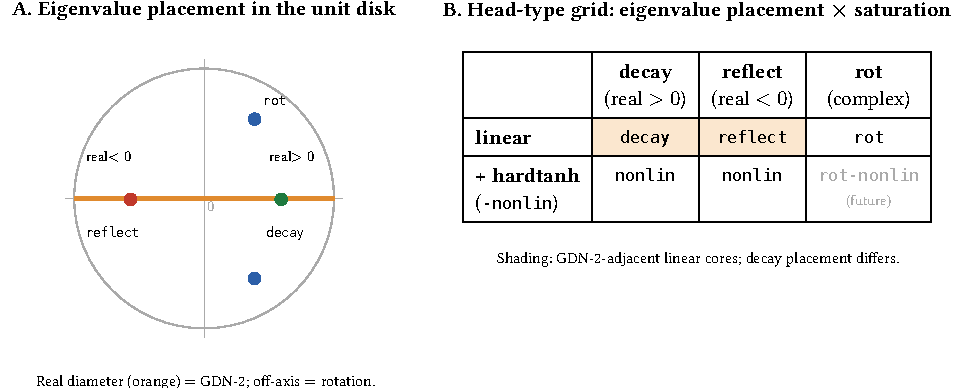
\includegraphics[width=\linewidth]{assets/figure-1.pdf}
\caption{ \emph{The Emender head-type taxonomy: eigenvalue placement $\times $ saturation.} \emph{(A)} Each head is fixed by where its along-key eigenvalue sits in the complex unit disk --- real-positive \protect\path|decay|, real-negative \protect\path|reflect|, or complex \protect\path|rot| --- and by whether the state map is linear or saturated. The orange real diameter is the locus GDN-2 occupies. \emph{(B)} The two axes name five cells. Shading marks GDN-2-adjacent linear cores; the Emender also explores off-axis rotation (\protect\path|rot|) and saturated state maps (\protect\path|nonlin|) as a within-layer pool. This taxonomy is descriptive: different decay placement prevents an exact equal-parameter restriction of the production cores. \protect\path|rot-nonlin| is reserved for future work. E88/E97/E98/E99 are historical run tags, not architecture names. The GDN-2 corner of this grid is not a strawman: it is the mixer of the 1.3 B linear baseline of Section~\ref{sec:lm} (GDN2-MLP), selected by the same search protocol as E97. }\label{fig_taxonomy}
\end{figure}





\section{Architecture}\label{sec:arch}



\subsection*{Per-head update}


Section~\ref{sec:intro} named the emender layer by what it does --- read what the memory predicts at the addressed slot, compute the prediction error, and write the correction --- and named E97 as the 1.3 B instance carried through the paper. This section makes the layer concrete: the per-step computation, the choices that fix it, and the shape numbers that make E97 one specific member of the family.

An emender layer runs $H $ independent heads side by side. Each head $h $ owns its own matrix-state memory ${S }_{h } \in  {\mathbb{R} }^{N  \times  V }$ --- the matrix state of Section~\ref{sec:background}, here addressed by an $N $-dimensional key and holding a $V $-dimensional value at each addressed slot. (Section~\ref{sec:formal}'s resource theorems use a single symbol $d $ for the common matrix dimension; in E97, $d  =  N  =  V  =  32$, so each head's memory is a $32 \times  32$ tile.) At each token, the layer's input projections supply, per head, a key ${k }_{h }$ and query ${q }_{h }$ in ${\mathbb{R} }^{N }$ that name the slots to write and read, a value ${v }_{h } \in  {\mathbb{R} }^{V }$ to store, a scalar decay ${d }_{h } \in  ( 0, 1) $ that fades the old state, and an output gate ${g }_{h } \in  {\mathbb{R} }^{V }$. E97 extends the E88 cell's write with two input-dependent gates, split along the two axes of the matrix state: a key-axis \emph{erase/read} gate ${e }_{h } \in  {( 0, 1) }^{N }$ that scales the address under which the old content is retrieved, and a value-axis \emph{write} gate ${w }_{h } \in  {( 0, 1) }^{V }$ that scales what is written (the GDN-2-inspired half of the design; Section~\ref{sec:formal}'s split-gated theorem set pins the relationship). The display below is one head's full step in execution order: normalize the two addresses, gate the read address and the write value, read the memory, form the retrieval error, update the bounded state, and gate the read output. The abstract witnesses of sets C/C\ensuremath{^{\prime}}/G in Section~\ref{sec:formal} use broader key/gate/state domains than this production step; they are not its reachable-trajectory proofs.


\[\begin{aligned}{k }_{h } &\leftarrow  \frac{\text{silu}( {k }_{h }) }{{\Vert \text{silu}( {k }_{h }) \Vert }_{2}} \quad  ( {\text{L}}^{2} \text{-normalized key}) \\ {q }_{h } &\leftarrow  \frac{\text{silu}( {q }_{h }) }{{\Vert \text{silu}( {q }_{h }) \Vert }_{2}} \quad  ( {\text{L}}^{2} \text{-normalized query}) \\ {e }_{h } &=  \sigma ( {E }_{h } {x }_{t })  \quad  ( \text{key-axis erase/read gate}) \\ {w }_{h } &=  \sigma ( {W }_{h } {x }_{t })  \quad  ( \text{value-axis write gate}) \\ {r }_{h } &=  {S }_{h }^{T } ( {e }_{h } \odot  {k }_{h })  \quad  ( \text{gated read at the key}) \\ {\delta }_{h } &=  {w }_{h } \odot  {v }_{h } -  {r }_{h } \\ {{S }'_{h }} &=  \operatorname{tanh}( {d }_{h } {S }_{h } +  {k }_{h } {\delta }_{h }^{T })  \\ {y }_{h } &=  \text{silu}( {g }_{h })  \odot  {( {{S }'_{h }}) }^{T } {q }_{h }\end{aligned}\]


Here $\text{silu}$ is the smooth pointwise activation $x  \odot  \sigma ( x ) $, with $\sigma $ the logistic sigmoid, ${v }_{h }$ is the post-activation value input (the $\text{silu}( v ) $ of the E88 cell, so the write gate scales an already-activated write), and ${\Vert \cdot \Vert }_{2}$ is the Euclidean norm. The first two lines put the key and query on the unit sphere so the addressing is bounded; the middle lines make the write a correction against the content already read --- under a gated address and at a gated magnitude --- rather than a raw addition; and the final line gates only the read output. With both split gates fixed to one (${e }_{h } = =  1$, ${w }_{h } = =  1$) the step specializes exactly to the E88 cell (Lean: \protect\path|SplitGatedDelta.e97_specializes_to_e88_all_one_gates_direct|), which is how the predecessor instance was defined; the state stays inside $\operatorname{tanh}$, so the update is nonlinear-state for every gate setting. This is the per-head primitive. Algorithm 1 spells out the same read-before-write order; its inputs are the projected quantities described above, and its output uses the returned state. It is not a full-stack implementation.

\emph{Algorithm 1 --- E97 per-head step.}
\begin{verbatim}
Input: S, projected k, q, activated v, d, e, w, g
1. k <- silu(k) / norm2(silu(k))
2. q <- silu(q) / norm2(silu(q))
3. r <- transpose(S) (e hadamard k)
4. delta <- (w hadamard v) - r
5. S_next <- tanh(d S + outer(k, delta))
6. y <- silu(g) hadamard (transpose(S_next) q)
Return: S_next, y
\end{verbatim}


E97 repeats it across a residual stack rather than changing the per-head equation.

E97 fixes these family choices to one billion-parameter instance: model width 1792, depth 11, $H  =  216$ heads per layer, $N  =  V  =  32$, expansion 1.0, a bias-free SwiGLU MLP of hidden width 4,032 after each mixer (mlp ratio 2.2623), per-rank batch size 4, a recurrence chunk length of 2048 tokens, and 1,286,589,072 parameters in total ($1\{ , \} 048\{ , \} 152\{ , \} 720$ non-MLP plus $238\{ , \} 436\{ , \} 352$ in the eleven MLPs). A Lean 4 definition (\protect\path|emender_1p27B|) pins the corresponding counts for the E88 predecessor geometry --- twelve layers of 370 heads, each with a $32 \times  32$ tile, yielding 22,200 independent recurrent programs per token at batch size 5 and $370 \times  ( 32 \times  32) $ recurrent-state scalars per layer --- and the same arithmetic gives E97's counts directly: at depth 11, $H  =  216$, and batch size 4 the stack runs $11 \times  216 \times  4 =  9\{ , \} 504$ independent recurrent programs per token, each carrying a $32 \times  32$ state tile ($216 \times  ( 32 \times  32) $ recurrent-state scalars per layer). Around the recurrent core the language-model wrapper is conventional --- a pre-norm residual stack with a final normalization and tied input/output embeddings. Heads never share recurrent state; each layer learns its own key, query, value, decay, split-gate, and output-gate projections; and the recurrent state starts at zero when no prior state is carried in.


\begin{figure}[htbp]
\centering
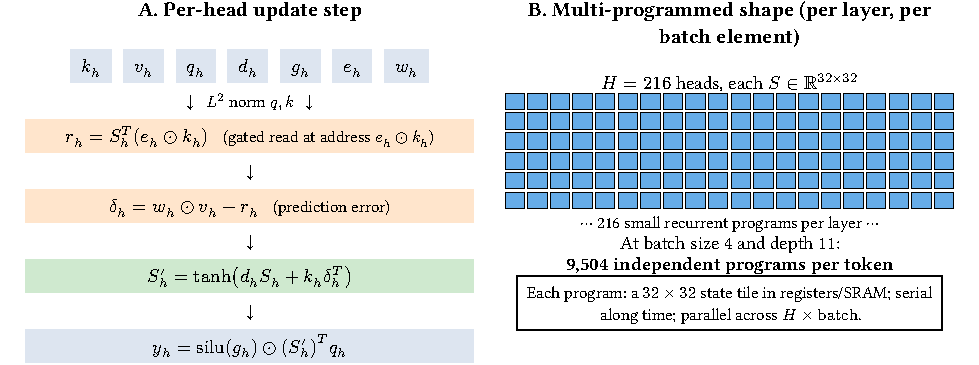
\includegraphics[width=\linewidth]{assets/figure-2.pdf}
\caption{ \emph{Emender architecture and multi-programmed shape.} \emph{(A)} Per-head recurrent dataflow (E97). Each head owns a small bounded associative matrix memory ${S }_{h }$. The model reads under the gated address ${e }_{h } \odot  {k }_{h }$, computes a prediction error ${\delta }_{h }$ against the gated write value, writes the bounded delta correction into ${S }_{h }$, and gates the read at ${q }_{h }$ for output. The $\operatorname{tanh}$ on the state, the delta-correcting write, the split erase/write gates, and the ${L }^{2}$-normalization of $q , k $ are visible here; Section~\ref{sec:arch} enumerates the four load-bearing ingredients of the Emender family. \emph{(B)} The 1.3 B stack exposes 216 small independent heads per layer per batch element. Each head is a $32 \times  32$ state tile that fits in registers/SRAM and runs its time loop serially; parallelism is harvested across heads, depth and batch (Section~\ref{sec:systems}), giving $11 \times  216 \times  4 =  9\{ , \} 504$ programs per token at batch size 4. The Lean theorem \protect\path|emender_1p27B_programs_per_batch_token_bs5| certifies the corresponding count (22,200) for the E88 predecessor geometry. }\label{fig_arch}
\end{figure}


For the Emender family, four ingredients are load-bearing; E97 uses all four in the instance above.




\begin{enumerate}[label=(\alph*)]
\item \emph{Bounded matrix state via $\operatorname{tanh}$ on $S $.} The state-channel duality (Section~\ref{sec:formal}) distinguishes the executed nonlinear composition from an affine fold; placing the non-linearity on the state itself, not only on a gate or the output, is what makes an emender layer nonlinear-state.
\item \emph{Delta-correcting write $w  \odot  v  -  {S }^{T } ( e  \odot  k ) $.} The emender layer reads what memory predicts at the gated address $e  \odot  k $, computes the prediction error $\delta $ against the gated write value $w  \odot  v $, and writes the correction. Under unit decay and all-one gates, the pre-$\operatorname{tanh}$ core with orthonormal keys gives exact overwrite at one slot while preserving orthogonal slots (\protect\path|linearDeltaWrite_overwrites_one_preserves_others|); full-state $\operatorname{tanh}$, split gates, and arbitrary keys change that guarantee. A raw-write update $S  \leftarrow  S  +  k  {v }^{T }$ (the M\textsuperscript{2}RNN family) accumulates without correction and cannot, with fixed weights, satisfy a uniform one-step overwrite specification (Section~\ref{sec:formal}).
\item \emph{Saturation latching of the $\operatorname{tanh}$ bound.} A slot driven near $\pm  1$ resists perturbations under the saturation theorem's hypotheses; sign-preserving hold and counter-delta release have separate decay and write-budget assumptions. These motivate revisable memory rather than guarantee persistent bindings in production E97. Section~\ref{sec:formal}'s Theorem set F (saturation insensitivity, sign-preserving hold, counter-delta release) formalizes all three as slot-wise statements on the full emender-layer update.
\item \emph{Many small heads, not one large matrix.} E97 at 1.3 B uses $H  =  216$ heads of $32 \times  32$ each ($11 \times  216 \times  4 =  9\{ , \} 504$ independent programs per token at batch size 4; the E88 predecessor's 22,200-at-batch-5 count is Lean-witnessed by \protect\path|RecurrentResourceFormalism.emender_1p27B_programs_per_batch_token|). Per-head ${L }^{2}$-normalized $q , k $ give many independent addressing programs and avoid the gradient-conditioning failure mode seen when a single shared $q , k $ pair feeds hundreds of value heads.
\end{enumerate}

\subsection*{GDN2-MLP state channel}


Algorithm 2 defines the adjacent GDN-2 linear core used by the formal comparison: decay is applied \emph{before} retrieval and correction, and no $\operatorname{tanh}$ is applied to the returned state. Its inputs are an already supplied key, split gates, value, and pre-decay matrix; it does not impose E97's projection processing on GDN2-MLP. In the trained stack the mixer is followed by the SwiGLU MLP of Section~\ref{sec:lm}, not by a state activation. This core specification does not assert that a multilayer stack has input-only gates.

\emph{Algorithm 2 --- GDN-2 split-gated linear core.}
\begin{verbatim}
Input: S, D, k, e, w, v
1. P <- D S
2. r <- transpose(P) (e hadamard k)
3. delta <- (w hadamard v) - r
4. S_next <- P + outer(k, delta)
Return: S_next
\end{verbatim}



\subsection*{Parameterization choices}


E97 parameterizes the per-head decay ${d }_{h }$ in log space, following Mamba2 \citep{mamba2_2024}: each head learns a scalar ${A }_{\operatorname{log}}$ and a bias ${\delta }_{\text{bias}}$ --- the code names \protect\path|A_log| and \protect\path|dt_bias| --- and forms the decay as $d  =  \operatorname{exp}( - \operatorname{exp}( {A }_{\operatorname{log}})  \cdot  \text{softplus}( \alpha ( x )  +  {\delta }_{\text{bias}}) ) $, where $\alpha ( x ) $ is the input-dependent term and $\sigma $ is again the logistic sigmoid. Both decay parameters are exempt from weight decay, as is standard for such timescale parameters, so the regularizer does not pull the learned decay toward a default. The recurrence is computed in float32 and cast back to the storage precision, and the $\operatorname{tanh}$ on the state uses the numerically stable form $\operatorname{tanh}( z )  =  2 \sigma ( 2 z )  -  1$ in the fused kernel to avoid overflow at large pre-activations. Three remaining choices are deliberate omissions rather than additions: there is no output normalization inside the recurrent layer --- an ablation removed it for a 0.10-nat gain, and the wrapper's block-level pre-norm plus final norm suffice --- no short convolution on the input, and, for the E88 predecessor, no write gate. E97 adds the split erase/read and write gates above; its output gate $\text{silu}( g ) $ still acts on the read alone.


\subsection*{The 1.3 B stack}


The 1.3 B stack's shape is not arbitrary. Ingredient (d) sets its character --- many small heads rather than one large matrix --- and the numbers follow from it: each head's $32 \times  32$ tile is small enough to live in registers (Section~\ref{sec:systems}), the head count $H  =  216$ is large enough to give that many independent addressing programs per layer, and eleven such layers --- each followed by its SwiGLU MLP, the channel-mixer that pairs with the token-mixing recurrence --- reach the 1.3 B-class budget the paired comparison fixes. The exact values were set by the per-architecture search of Section~\ref{sec:lm}, not by hand. At batch size 4, depth 11 and $H  =  216$ multiply to $11 \times  216 \times  4 =  9\{ , \} 504$ independent recurrent programs per token, each carrying its own $32 \times  32$ state tile. The reference implementation and the fused Triton recurrence kernel that steps these tiles are listed in the Appendix.


\subsection*{Architectural contrasts: delta correction and state nonlinearity}


Three architectural properties are candidates for the one that lets a model track state: \emph{matrix state}, \emph{temporal nonlinearity on that state}, and \emph{delta correction in the write}. The closest update-rule comparator to the Emender in the literature is M\textsuperscript{2}RNN \citep{m2rnn2026}. Its nonlinear matrix-state update has two parts, written here as one display: the first line builds a nonlinear write candidate ${Z }_{t }$ from the matrix state ${H }_{t - 1}$, a learned weight $W $, and the current key--value outer product ${k }_{t } {v }_{t }^{T }$; the second blends that candidate back into the state through a forget gate ${f }_{t }$.


\[\begin{aligned}{Z }_{t } &=  \operatorname{tanh}( {H }_{t - 1} W  +  {k }_{t } {v }_{t }^{T }) \\ {H }_{t } &=  {f }_{t } {H }_{t - 1} +  ( 1 -  {f }_{t })  {Z }_{t }. \end{aligned}\]


Algorithm 3 makes the displayed scalar-forget version explicit. The row/column/cell external-forget resource classes in Section~\ref{sec:formal} retain their separately stated broadcasting signatures; this is not a substitution for those quantified definitions.

\emph{Algorithm 3 --- raw-write nonlinear comparator step.}
\begin{verbatim}
Input: H, fixed W, k, v, scalar forget gate f
1. Z <- tanh(H W + outer(k, v))
2. H_next <- f H + (1 - f) Z
Return: H_next
\end{verbatim}


That split is exactly what the Emender cell lacks: its carry sits inside the bounded delta-correcting update, and E97's split gates act inside the delta path rather than blending an external carry with a candidate. M\textsuperscript{2}RNN is \emph{nonlinear-state} by the criterion of Section~\ref{sec:background}, since ${H }_{t - 1}$ appears inside $\operatorname{tanh}$ via ${H }_{t - 1} W $, but the write into $H $ is a raw outer product $k  {v }^{T }$ rather than a delta correction. A three-row structural comparison shows the shared and distinct ingredients; it is not a causal ablation:


\begin{table}[htbp]
\centering
\begingroup\setlength{\tabcolsep}{3pt}
\begin{tabularx}{\linewidth}{|>{\hsize=1.25000\hsize\linewidth=\hsize\raggedright\arraybackslash}X|>{\hsize=0.62500\hsize\linewidth=\hsize\raggedright\arraybackslash}X|>{\hsize=0.62500\hsize\linewidth=\hsize\raggedright\arraybackslash}X|>{\hsize=0.62500\hsize\linewidth=\hsize\raggedright\arraybackslash}X|>{\hsize=1.87500\hsize\linewidth=\hsize\raggedright\arraybackslash}X|}\hline
\emph{Property} & \emph{GDN} & \emph{M\textsuperscript{2}RNN} & \emph{Emender} & \emph{What it shows} \\ \hline
Matrix state & yes & yes & yes & Cannot separate: GDN has it and fails ${S }_{5}$ \\ \hline
Temporal nonlinearity on state & no & yes & yes & Cannot separate: M\textsuperscript{2}RNN-CMA stalls at 0.22 on ${S }_{5}$ \\ \hline
Delta correction in write & yes & no & yes & Distinguishes delta from raw-write, not GDN from Emender \\ \hline
\end{tabularx}
\endgroup

\caption{ \emph{Structural comparison, not causal elimination.} Matrix state is shared by all three families; temporal state nonlinearity is shared by M\textsuperscript{2}RNN and the Emender; delta correction is shared by GDN and the Emender. The ${S }_{5}$ ordering (0.79 / 0.36 / 0.22, Section~\ref{sec:expressivity}) motivates testing their combination, but does not isolate every architectural choice. }\label{tab_ablation}
\end{table}


Two checks motivate, rather than prove, a learning-efficiency reading. M\textsuperscript{2}RNN-CMA reaches only 0.31 on solvable ${S }_{3}$, so non-solvability alone cannot explain its shortfall. At the 8 M shape, the recurrent state has 131,072 scalars versus the ${\operatorname{log}}_{2} 6 \approx  2.6$-bit information floor. That headroom rules out a bare state-count shortage, not constrained realizability or optimization failure. The formal counterpart is the matched-signature mixed-key one-step separation (\protect\path|emender_m2rnn_one_step_resource_separation_embeds|, Section~\ref{sec:formal}), not a trained-model accuracy guarantee. Delta correction distinguishes the Emender from raw-write; nonlinear state distinguishes it from GDN, which also uses a delta correction.


\section{Multi-Programming and Systems}\label{sec:systems}



\subsection*{Multi-programming: the throughput-enabling design choice}


Throughput comes from width, not from time. A linear recurrence earns its throughput on the \emph{time axis}: because ${S }_{t } =  {A }_{t } {S }_{t - 1} +  {b }_{t }$ unfolds into a product that depends on the inputs alone, the step-by-step loop can be re-expressed as a prefix scan or a chunkwise matrix multiplication over the whole sequence at once. A purely nonlinear recurrence cannot be rewritten that way without giving up the nonlinear update that makes it expressive, so its time loop has to run serially. \emph{Multi-programming} recovers the throughput on the other axis. Rather than parallelize one recurrence along time, it replicates the recurrent computation across many independent heads --- each with its own small bounded matrix state --- and harvests parallelism across those heads, across state tiles, and across batch elements, while the time loop inside each head still runs one step at a time.

The design choice is a decoupling: it frees throughput from the \emph{shape} of the update. The recurrent body must stay a bounded, register-resident per-step map at a fixed matrix-state signature --- that is what keeps each head cheap --- but it need not be compatible with an associative scan or a chunkwise WY product. The cost is paid in per-head serial time, most exposed at long sequence lengths where the serial loop is longest; the gain is that a nonlinear recurrence can keep a modern accelerator busy with no time-axis scan at all. The route is agnostic to the update rule: both pure-nonlinear instances of the predecessor cohort --- the Emender and the raw-write M\textsuperscript{2}RNN-CMA --- have geometries consistent with the same simple resource predicate. The named Lean theorem \protect\path|RecurrentResourceFormalism.multiProgrammed_admits_m2rnn_and_emender| checks E88 and a different M\textsuperscript{2}RNN proxy (depth 22, 70 heads, 256 state scalars/head), not the trained depth-21, 370-head M\textsuperscript{2}RNN-CMA. The latter satisfies the four signature-field conditions by inspection/arithmetic, not by this exact-instance theorem (Section~\ref{sec:formal}).


\subsection*{The 1.3 B Emender shape under multi-programming}


A modern GPU exposes many independent streaming multiprocessors, each able to run a small program out of its own registers and shared memory, and multi-programming is built to fill them. E97, the 1.3 B Emender instance, runs 216 such programs per layer per batch element --- one per head --- so at depth 11 and batch size 4 the layer stack issues $11 \times  216 \times  4 =  9\{ , \} 504$ small independent recurrent programs per token, each carrying its own $32 \times  32$ state tile small enough to live in registers. Keeping the accelerator busy therefore asks nothing of parallelism \emph{along time}: the parallelism across these programs is already enough to fill it. How fully it does is something the next section measures directly.


\subsection*{Measured throughput and utilization (CUDA only)}


All throughput measurements and throughput-budget smokes reported here are CUDA-only; none establishes correctness, performance, or parity on ROCm.

That the card stays busy is a claim about occupancy, and it is measured directly. Driving the 1.273 B E88 predecessor instance (batch 5, context 2048) through its own training path on a free NVIDIA RTX 6000 Ada (48 GB) and sampling \protect\path|nvidia-smi| once a second over a sustained post-warmup window, the GPU holds \emph{median 100\% utilization (mean 99.8\%, minimum 96\% across 133 samples)} while drawing 97\% of its 300 W power cap. The accelerator stays busy on width-axis multi-programming alone, with no time-axis scan. Sustained throughput is \emph{7,492 tokens/s} (mean over steady 50-step windows; median 7,468); a slower sibling GPU sustained 7,277 tokens/s, so the absolute figure is GPU-dependent at the few-percent level. E97 uses the shared E88-derived Triton engine with split-edit inputs, but the E88 occupancy measurement is not an E97 occupancy measurement.

At the literal 1.3 B pair geometry the two arms are measured head to head: on a leased RTX 6000 Ada under identical conditions, E97-MLP sustains 3,211 tokens/s per GPU at batch 4 against 3,290 for GDN2-MLP --- a \emph{0.976\ensuremath{\times} tie} --- while using 28.9 GB against GDN2-MLP's 35.7 GB peak memory, so E97 fits batch 6 (4,470 tokens/s per GPU) where GDN2-MLP OOMs (\protect\path|experiments/preflight_100b/RESULTS.md|). The Emender's edge at this scale is memory, not kernel speed; an earlier 1.26--1.56\ensuremath{\times} speedup measured at small grok-scale dims is \emph{not} reproduced at 1.3 B.

This figure is occupancy, not peak arithmetic, and the two should not be run together. Model-FLOPs utilization (MFU) --- computed with the standard $6N $ convention against the card's dense bf16 peak of 364 TFLOPS --- is \emph{15.7\%}, and that is a conservative lower bound: $6N $ counts only the weight-matmul FLOPs and excludes the recurrence and gate operations, so the true MFU is slightly higher. High occupancy with modest MFU is the expected profile of a model bound by memory bandwidth and the serial recurrence rather than by arithmetic: the GPU is busy nearly all of the time but converts about 16\% of its peak FLOPs into useful work.

What that throughput buys on the width axis is best read against a real time-axis kernel. A chunkwise linear-scan baseline --- Gated DeltaNet as implemented in the flash-linear-attention (FLA) library (1.352 B, the CMA-matched shape of the predecessor cohort), run on the same GPU, context, and time budget --- sustains 8,248 tokens/s at MFU 18.4\% and the same near-100\% occupancy. The E88 predecessor reaches \emph{\ensuremath{\approx} 91\% of that linear-scan kernel's tokens/s} (7,492 / 8,248) \emph{without performing the sequential time-axis scan at all}. Width-axis multi-programming therefore recovers linear-scan-class throughput on the width axis. It does not beat the chunked-scan kernel on raw tokens/s --- FLA is about 10\% faster here, at a slightly larger parameter count and a different batch --- so the standing is parity-class, not superiority.


\subsection*{Fused Triton recurrence kernel}


The forward kernel uses an internal \protect\path|[T, B, H, *]| layout (time, batch, head, $\ldots $) and dispatches one program per \protect\path|(batch, head_block)|. The \protect\path|BLOCK_H| parameter is autotuned over $\{ 1,  2,  4,  8,  16\} $ because at $H  \geq  256$ per-program-per-head launch overhead dominates. The state tile lives in registers and shared memory for the duration of the $T $-step loop. The following pieces are fused into the same Triton program: $\operatorname{tanh}$/$\text{silu}$ activations on input projections, ${L }^{2}$ normalization of $q ,  k $, the recurrent delta write, and the output gate. Each fusion removes one to two \protect\path|torch.cuda| launches per layer call; at depth 12 the aggregate saving is approximately 50--60 ms per step.


\subsection*{Sparse-checkpoint backward}


The forward kernel saves $S $ only every $K  =  16$ steps. The backward kernel processes one $K $-step segment at a time: it forward-replays the $K $ steps to rebuild per-step ${S }_{t - 1}$ from the saved checkpoint, then walks backward to apply the chain rule. The activation memory used by the kernel is $\frac{T }{K } +  1$ checkpoint slots instead of $T $. At $K  =  16$ this is approximately a $16 \times $ shrink, at the cost of a single extra forward pass per segment.


\subsection*{Triton source portability; CUDA-only validation}


The kernel is written in Triton \citep{triton2019}, a source-portability route rather than evidence of cross-backend parity. The pair's production runs, kernel throughput measurements, and expressivity throughput smokes all ran on NVIDIA CUDA. No ROCm smoke or paired production artifact supports a correctness or throughput claim here; no CUDA/ROCm parity is claimed. The successor E97 Frontier continuation is a separate, single-arm line of work, not a portability benchmark for the E97/GDN2-MLP pair.


\subsection*{Distributed training}


The 1.3 B-class result reported here was produced on a single eight-GPU workstation, with no cluster and no sequence parallelism --- both 150 B-token arms of Section~\ref{sec:lm} ran the same \emph{local DiLoCo} recipe on that one machine: eight independent islands (one per GPU), schedule-free AdamW \citep{schedulefree2024} inside each island, and plain model-weight averaging across islands every $\tau  =  250$ local steps (outer learning rate 1.0, momentum 0 --- the conservative plain-average form of DiLoCo \citep{diloco2023}). Scaling the same recipe past one machine pairs schedule-free AdamW per island with hierarchical local-SGD averaging: each island is one node of 8 GPUs with intra-island DDP, and inter-island synchronization averages model weights on the same $\tau  =  250$ cadence. The structural point holds either way: because the Emender's parallelism is across programs rather than along time, it does not need sequence parallelism to stay competitive at the 1.3 B-class --- a simplification relative to the chunked-scan implementations that linear-state recurrences rely on.

A different route would parallelize the time loop itself. ParaRNN \citep{pararnn2025} does so with Newton's method on a block-bidiagonal Jacobian; we tried it on the $\operatorname{tanh}( d  S  +  k  {\delta }^{T }) $ map at $32 \times  32$ block size and found it markedly slower in throughput than the multi-programmed Triton kernels above. Newton iteration carries a data-dependent solve count per step, and its convergence on the bounded $\operatorname{tanh}$ map is unestablished, whereas multi-programming is a single serial pass per head.


\section{Language-Modeling Results}\label{sec:lm}



\subsection*{The 1.3 B double-pairing: setup and training identities}


The 1.3 B comparison is a \emph{pairing}: one nonlinear-state model and one linear-state model, each selected by its own CMA-ES search, trained from scratch under a literally identical recipe, and read out at exactly matched aggregate tokens. The two arms are E97 --- the Emender split-edit instance of Section~\ref{sec:arch}, paired with a bias-free SwiGLU MLP per layer --- and GDN2-MLP --- the official-style Gated DeltaNet-2 \citep{gated_deltanet2_2026} mixer with the \emph{same} SwiGLU MLP, bound to external source commit \protect\path|95709fc|. Holding the channel-mixer (MLP) fixed on both arms is what makes this a comparison of token mixers --- the recurrence --- rather than of everything at once.


\begin{table}[htbp]
\centering
\begingroup\setlength{\tabcolsep}{3pt}
\begin{tabularx}{\linewidth}{|>{\hsize=0.63636\hsize\linewidth=\hsize\raggedright\arraybackslash}X|>{\hsize=1.18182\hsize\linewidth=\hsize\raggedright\arraybackslash}X|>{\hsize=1.18182\hsize\linewidth=\hsize\raggedright\arraybackslash}X|}\hline
\emph{Training identity} & \emph{E97-MLP} & \emph{GDN2-MLP} \\ \hline
Parameters & 1,286,589,072 & 1,286,713,448 (+0.0097\%) \\ \hline
Mixer & Emender split-edit delta (Section~\ref{sec:arch}) & Gated DeltaNet-2, 4-token conv \\ \hline
Geometry & dim 1792, depth 11, $H  =  216$, $N  =  V  =  32$, mlp ratio 2.2623 & dim 2176, depth 12, $H  =  30$, expansion 1, mlp ratio 3.2587 \\ \hline
Base LR (CMA-selected) & $1.007 \times  {10}^{- 3}$ & $4.743 \times  {10}^{- 4}$ \\ \hline
Data & The Pile, 2,048-token chunks, \protect\path|p50k_base| & identical \\ \hline
Optimizer & schedule-free AdamW, bf16, per-rank batch 4 & identical \\ \hline
DiLoCo & 8 islands (one per GPU), $K  =  250$, plain average, outer lr 1.0, $\beta  =  0$ & identical \\ \hline
Tokens per optimizer step & $8 \times  4 \times  2048 =  65\{ , \} 536$ & identical \\ \hline
Run & \protect\path|emender_E97_1.3B_20260709_084606| & \protect\path|gdn2_gdn2-mlp_1.3B_20260722_083444| \\ \hline
Final step & 2,300,930 & 2,323,616 \\ \hline
Final aggregate tokens & 150,793,748,480 & 152,280,498,176 \\ \hline
Final last-100 loss (nats/token) & 2.4365 & 2.4034 \\ \hline
Source .pt checkpoint SHA-256 & \protect\path|0239706e1f67e4823008a3a2754894b5
b94dc1663580d2e40c1c74f7dd6a72b2| & \protect\path|ffae61cfeeeff820f469f7d66dd31c60
e48c455872ff9102e57b15ad75bad59b| \\ \hline
\end{tabularx}
\endgroup

\caption{ \emph{Training identities of the 1.3 B pair.} Both arms ran the same launcher harness on the same eight-GPU workstation: same data file, chunk size, tokenizer, optimizer, DiLoCo policy, token cadence, and checkpoint cadence (saves every 500 steps, on merge boundaries); the arms differ only in mixer, geometry, and the CMA-selected learning rate. Sources: launch manifests \protect\path|scripts/launch_emender_8gpu_diloco.sh| and \protect\path|scripts/launch_gdn2_mlp_8gpu_diloco.sh|; per-run \protect\path|args.json|/release validation receipts (\protect\path|docs/EMENDER_DILOCO_OPS_HANDOFF_20260722.md|, \protect\path|docs/validation/e97-huggingface-dense-base-and-cli-agent-release.md|, \protect\path|docs/validation/gdn2-huggingface-152b-control-release.md|). }\label{tab_pair_identities}
\end{table}


Both arms consumed 65,536 tokens per optimizer step (8 ranks $\times $ batch 4 $\times $ chunk 2,048, validated from the launch manifests and log deltas), so matched optimizer steps \emph{are} matched aggregate tokens. GDN2-MLP was run 1.49 B tokens past E97's final step so that the comparison could be read near E97's terminal authority. The final common logged read-out is five optimizer steps earlier than that checkpoint; no paired loss statistic uses GDN2's extra tokens.

Algorithm 4 separates selection, training, and comparison. It summarizes the recorded pair protocol rather than specifying a new search or training run; the historical CMA sweep table below identifies retained and missing winner-search records. The averaging window is reported, not selected to establish an ordering.

\emph{Algorithm 4 --- pair selection, training, and loss alignment.}
\begin{verbatim}
Input: per-family search bounds, candidate budget, Pile recipe
1. For each family, run CMA-ES with its candidate budget.
   Train candidates; score the recorded late-loss window.
   Retain the winner geometry and learning rate.
2. Train each winner on the common chunk/tokenizer recipe.
   Each island takes local schedule-free AdamW steps.
   Every 250 steps, average parameters (outer LR 1, beta 0).
   Record rank-0 losses and merge-boundary checkpoints.
3. Deduplicate each loss log by optimizer step.
4. Intersect logged step IDs through the common cutoff.
5. Compute raw and declared trailing-window loss differences.
Return: pair identities, aligned losses, windowed differences
\end{verbatim}



\subsection*{Loss parity at matched tokens}


The primary read-out is the training-log loss of both arms aligned on exact common logged steps through step 2,300,925 (150,793,420,800 tokens): 92,037 aligned records, zero E97-only and zero GDN2-only records through the cutoff, no interpolation. This is 327,680 tokens (five optimizer steps) before E97's terminal checkpoint at step 2,300,930; the table is a last-common-log comparison, not an unlogged terminal-step measurement.


\begin{table}[htbp]
\centering
\begingroup\setlength{\tabcolsep}{3pt}
\begin{tabularx}{\linewidth}{|>{\hsize=1.60000\hsize\linewidth=\hsize\raggedright\arraybackslash}X|>{\hsize=0.80000\hsize\linewidth=\hsize\raggedright\arraybackslash}X|>{\hsize=0.80000\hsize\linewidth=\hsize\raggedright\arraybackslash}X|>{\hsize=0.80000\hsize\linewidth=\hsize\raggedright\arraybackslash}X|}\hline
\emph{Statistic at the 150.79 B-token cutoff} & \emph{E97} & \emph{GDN2-MLP} & \emph{$\Delta $ (GDN2 $- $ E97)} \\ \hline
Raw loss at cutoff step & 2.4770 & 2.4324 & $- 0.0446$ \\ \hline
80-point trailing smoothed & 2.4370 & 2.4267 & $- 0.0103$ \\ \hline
Mean, last 100 steps & 2.4284 & 2.4423 & $+ 0.0139$ \\ \hline
Mean, last 1,000 steps & 2.4358 & 2.4273 & $- 0.0085$ \\ \hline
Early comparison, 5.118 B tokens (smoothed) & 2.9300 & 2.8588 & $- 0.0713$ \\ \hline
\end{tabularx}
\endgroup

\caption{ \emph{Matched-token loss comparison (nats/token, The Pile).} The common logged cutoff is step 2,300,925, not checkpoint step 2,300,930. At the matched cutoff the two arms sit within $0.010$ nats/token smoothed ($\approx  0.4\% $ relative), and the \emph{sign of the gap depends on the averaging window}: GDN2-MLP is lower on the full-trajectory and 1,000-step windows, E97 is lower on the most recent 100-step window. Early in training (5.1 B tokens) GDN2-MLP led by 0.071 nats; the gap closed as training progressed. Source: \protect\path|docs/GDN2_OPS_SNAPSHOT_20260728.md| (final matched cutoff) and \protect\path|docs/GDN2_E97_MATCHED_LOSS_COMPARISON_20260723.md| (early comparison); both parse rank-0 logs only, deduplicate by optimizer step, and align on exact common steps. }\label{tab_matched_loss}
\end{table}


The reading is \emph{parity}, and it is a null result of the same kind the predecessor cohort measured (Section~\ref{sec:appendix_cohort}): after both families are optimized by their own search and trained on literally the same tokens, bulk language-modeling loss does not distinguish the nonlinear-state from the linear-state recurrence. Under the run's recorded byte normalization (\protect\path|bytes/token| $=  3.783$ from the frozen \protect\path|args.json|), E97's final-window loss of 2.4365 nats/token corresponds to an estimated \emph{0.93 bits per byte} --- sub-1-bpb territory for a purely nonlinear recurrence.

Two boundaries on this measurement are stated plainly. First, it is a \emph{training-log} comparison: a held-out, tokenizer-invariant bpb measurement on the 150 B pair (as Section~\ref{sec:appendix_cohort} performs for the predecessor cohort) has not yet been run and is the pending evaluation item --- TODO-NEEDS-EVIDENCE. Second, it is one run per arm, single-seed; the window-dependent sign of the $\Delta $ in Table~\ref{tab_matched_loss} is the summary of a tie at this precision, not evidence for either ordering. The search process behind this parity binding is decomposed per retained sweep in Table~\ref{tab_cma_sweeps}; the historical snapshots are not silently substituted for the carried-in winner searches, whose missing first-generation fitness is tracked as Open item U3.1 below.


\subsection*{The convergent-loss null already appears at search scale}


The 150 B parity extends a null that is visible much earlier and much more broadly. At the CMA-search stage --- five CMA-best 1.3 B models at their own found geometry, one fixed held-out Pile-tail slice of 131,072 scored tokens, and the same 15-minute per-candidate training budget the searches used --- all five architectures land in a 0.088-bpb held-out band: pure-E97 2.0126, M\textsuperscript{2}RNN 2.0344, Emender-mix 2.0402, E97-MLP 2.0911, GDN2-MLP 2.1013 bits per byte (non-averaged weights, the basis consistent with the search fitness; \protect\path|experiments/lb_compare_20260613/LEADERBOARD.md|). Within that band E97-MLP is ahead of GDN2-MLP on \emph{both} primary metrics --- search fitness 5.8606 vs 5.8949 and held-out bpb 2.0911 vs 2.1013 --- but the statement is descriptive closeness with the reported ordering, not a statistically established win or equivalence: bulk loss occupies a narrow observed band across the tuned families, and the distinguisher must be capability (Section~\ref{sec:expressivity}), not loss.


\subsection*{Matched-control transparency: search breadth, budgets, and configurations}


Because the central 1.3 B claim is a \emph{null} on loss, the credibility of the baseline is load-bearing: a reader must be able to verify that GDN2-MLP was optimizer-hardened, not strawmanned. The full provenance chain is as follows.

\emph{Search protocol (all families).} Each family was searched with the same driver (\protect\path|scripts/cmaes_search_v2.py|): CMA-ES \citep{cmaes2003} with population 8 over the family's structural knobs (width, depth, head count, state width, learning rate, batch size), 15 minutes of training per candidate at 2,048-token context on The Pile with \protect\path|p50k_base| (vocab 50,281), bf16 with fused kernels mandatory (no eager fallback), at a 1,300 M-parameter target with $\pm  3\% $ tolerance. Fitness is the candidate's mean training loss over the 15-minute trajectory; ties are broken by nothing else.

\emph{Search breadth.} The corrected 1.3 B redo sweep covered \emph{eleven families} with 64--128 completed evaluations each (\protect\path|docs/E97_RAW_1P3B_LEADERBOARD.md|): \protect\path|e97-raw| (103 evals, best avg loss 5.9511), \protect\path|gdn2-mlp| (64, 5.9613), \protect\path|e97| (109, 5.9733), \protect\path|e88-linear| (104, 5.9854), \protect\path|e88| (92, 5.9900), \protect\path|e88-raw| (106, 6.0390), \protect\path|e97-linear| (109, 6.0516), \protect\path|fla-gdn| (109, 6.0854), \protect\path|m2rnn| (107, 6.1161), mixer-only \protect\path|gdn2| (96, 6.3850), and \protect\path|transformer| (128, 6.4606) --- every family's best lands within a 0.5-nat band, and the transformer baseline was searched under the same budget rather than copied from the literature. The normalized corpus behind these sweeps --- 1,285 candidate trajectories across 13 family panels, 192,147 parsed step-loss rows, all inside the 15-minute candidate window --- is committed at \protect\path|paper/results/cmaes_burst_v2/| (per-family trajectory data and manifest in \protect\path|cmaes_trajectory_points.csv.gz|, \protect\path|cmaes_eval_summary.csv|).

\emph{The two carried-in winners.} E97-MLP carries the emender-mlp search winner (dim 1792, $H  =  216$, depth 11, n\_state 32, mlp ratio 2.2623, lr $1.007 \times  {10}^{- 3}$; search fitness 5.8606, \protect\path|experiments/lb_compare_20260613/REPRODUCTION.md|), and GDN2-MLP carries the \protect\path|lb-gdn2-mlp| winner (dim 2176, $H  =  30$, depth 12, expansion 1, mlp ratio 3.2587, lr $4.743 \times  {10}^{- 4}$; 104 completed evaluations over 13 generations, best fitness 5.8949 at eval 86, \protect\path|docs/repro/lb_gdn2_mlp_20260612/best.json|). One asymmetry is disclosed: in the earlier redo sweep the \protect\path|gdn2-mlp| arm had completed only 64 evaluations against the $>  96$ target, so its standing there was provisional; the committed \protect\path|lb_gdn2_mlp_20260612| search (104 evals) is the one the 150 B run launched from. M\textsuperscript{2}RNN was searched under the same protocol (fitness 6.1161 at 1.3 B) but is not a 150 B arm (Section~\ref{sec:intro}).

\emph{Per-sweep decomposition (U3).} For each retained sweep, report the number of candidate trajectories and generation records, the best candidate mean-loss fitness in generation zero, and the best observed fitness across the snapshot. Their difference is the within-sweep search gain, not a causal attribution of improvement to architecture or tuning. Complete, partial, and failed snapshots remain distinct. These earlier retained snapshots are not the later eleven-family leaderboard totals or the two carried-in winner searches.


\begin{table}[htbp]
\centering
\begingroup\setlength{\tabcolsep}{3pt}
\begin{tabularx}{\linewidth}{|>{\hsize=2.51799\hsize\linewidth=\hsize\raggedright\arraybackslash}X|>{\hsize=0.75540\hsize\linewidth=\hsize\raggedright\arraybackslash}X|>{\hsize=0.55396\hsize\linewidth=\hsize\raggedright\arraybackslash}X|>{\hsize=0.55396\hsize\linewidth=\hsize\raggedright\arraybackslash}X|>{\hsize=0.90647\hsize\linewidth=\hsize\raggedright\arraybackslash}X|>{\hsize=0.90647\hsize\linewidth=\hsize\raggedright\arraybackslash}X|>{\hsize=0.80576\hsize\linewidth=\hsize\raggedright\arraybackslash}X|}\hline
\emph{Sweep ID} & \emph{Status} & \emph{Evals} & \emph{Gens} & \emph{Gen-0 best} & \emph{Observed best} & \emph{Gain} \\ \hline
redo 1300m e88 & partial & 34 & 7 & 6.2124 & 6.1086 & 0.1038 \\ \hline
redo 1300m e97 & complete & 64 & 8 & 5.9980 & 5.9733 & 0.0247 \\ \hline
redo 1300m e97 linear & complete & 64 & 8 & 6.2218 & 6.0967 & 0.1250 \\ \hline
redo 1300m e97 raw & complete & 80 & 10 & 6.1658 & 5.9511 & 0.2146 \\ \hline
redo 1300m gdn2 & complete & 96 & 12 & 6.4741 & 6.3850 & 0.0891 \\ \hline
redo 1300m transformer & partial & 60 & 7 & 6.8822 & 6.5673 & 0.3149 \\ \hline
ctx2k e88 delta & complete & 128 & 16 & 6.1167 & 5.9974 & 0.1193 \\ \hline
ctx2k e88 raw & complete & 136 & 17 & 6.1702 & 6.0395 & 0.1307 \\ \hline
ctx2k fla gdn & complete & 160 & 20 & 6.3642 & 6.1104 & 0.2538 \\ \hline
ctx2k m2rnn home xma & complete & 144 & 18 & 6.2198 & 6.0626 & 0.1573 \\ \hline
ctx2k mamba2 & partial & 157 & 19 & 6.1704 & 6.0560 & 0.1144 \\ \hline
ctx2k transformer & complete & 160 & 20 & 5.9357 & 5.9046 & 0.0312 \\ \hline
emender e97 & failed & 1 & 0 & --- & 6.3260 & --- \\ \hline
emender gdn2 & failed & 1 & 0 & --- & 7.1571 & --- \\ \hline
Carried-in E97-MLP & U3.1 & --- & --- & --- & see prose & --- \\ \hline
Carried-in GDN2-MLP & U3.1 & see prose & see prose & --- & see prose & --- \\ \hline
\end{tabularx}
\endgroup

\caption{ \emph{Per-sweep CMA audit at the loss-parity binding.} Fitness and gains are nats/token, from retained candidate mean-loss fields, not the final long-run loss. Counts are snapshot coverage, including failed one-evaluation attempts; generation count is retained generation records, not an inferred total. The first 14 rows derive directly from \protect\path|paper/results/cmaes_burst_v2/cmaes_{eval,generation}_summary.csv| (\protect\path|899e91cd|), a different snapshot from the later leaderboard. U3.1 applies to the last two rows only, the carried-in E97-MLP and GDN2-MLP searches; they are not mapped to an earlier normalized sweep. GDN2-MLP's retained \protect\path|docs/repro/lb_gdn2_mlp_20260612/best.json| supplies its count and winner fitness in the provenance prose above, but not first-generation data. Dashes indicate unavailable fields, not zeros or no improvement. }\label{tab_cma_sweeps}
\end{table}


\emph{Open item U3.1 --- carried-in winner first-generation fitness unavailable; within-sweep gain not computable from retained artifacts.} This covers both final carried-in rows. First-generation spread is also unavailable; E97-MLP's candidate/generation totals are not retained in this normalized snapshot. Recover the winner searches' generation logs before computing these quantities; do not estimate them from the earlier sweeps.

\emph{One search per family, then one training run per family.} No post-search per-arm tuning was applied to either 150 B arm: the launchers freeze the searched geometry and learning rate verbatim (Table~\ref{tab_pair_identities}), so the arms' only degrees of freedom are the ones their own searches selected.

\emph{FLOPs-per-bit corroboration at 480 M.} The same protocol run at 480 M parameters over four recurrent families --- the vanilla nonlinear Elman cell (E1), E88, FLA-GDN, and Mamba2 --- shows the same null from the other side: independently tuned, the four families share one FLOPs-per-bit curve over more than two orders of magnitude of training FLOPs (final losses 1.14--1.34 nats at matched FLOP budgets; \protect\path|paper/results/cma_flop_rate/|). Once sensibly tuned, the choice of recurrent family changes \emph{what} is trained, not \emph{how much compute per bit} --- which is why the 1.3 B loss null is expected rather than surprising, and why the paper's positive claims live in Section~\ref{sec:expressivity} and Section~\ref{sec:formal}.


\subsection*{Downstream capability panels: a null, on the predecessor cohort}


No downstream capability evaluation of the 150 B E97/GDN2-MLP pair has been run yet (TODO-NEEDS-EVIDENCE). What exists is committed evidence from the predecessor 1.3 B racer cohort (E88, FLA-GDN, M\textsuperscript{2}RNN, Mamba2 --- Section~\ref{sec:appendix_cohort}), and it provides the reference comparison: at $\approx  1 M $-step training extents, on a 2,049-item multi-choice fact panel and a 2,048-item reasoning panel (BBH + ReCLor + FOLIO), the four architectures sit within a few percentage points of one another in narrow observed bands (Table~\ref{tab_downstream}), without a paired or seed-level equivalence test.


\begin{table}[htbp]
\centering
\begingroup\setlength{\tabcolsep}{3pt}
\begin{tabularx}{\linewidth}{|>{\hsize=1.66667\hsize\linewidth=\hsize\raggedright\arraybackslash}X|>{\hsize=0.83333\hsize\linewidth=\hsize\raggedright\arraybackslash}X|>{\hsize=0.83333\hsize\linewidth=\hsize\raggedright\arraybackslash}X|>{\hsize=0.83333\hsize\linewidth=\hsize\raggedright\arraybackslash}X|>{\hsize=0.83333\hsize\linewidth=\hsize\raggedright\arraybackslash}X|}\hline
\emph{Panel (predecessor cohort)} & \emph{E88} & \emph{FLA-GDN} & \emph{M\textsuperscript{2}RNN} & \emph{Mamba2} \\ \hline
Fact panel, 2,049 items (accuracy) & 0.345 & 0.373 & 0.358 & 0.353 \\ \hline
Reasoning panel, 2,048 items (accuracy) & 0.319 & 0.350 & 0.336 & 0.324 \\ \hline
\end{tabularx}
\endgroup

\caption{ \emph{Downstream panels at the predecessor cohort's training extent --- a null, reported as a null.} All four 1.3 B-class models are within $\approx  3.5$ percentage points on both panels; none has crossed the threshold where these benchmarks differentiate architectures. Measured on the predecessor E88-era checkpoints (steps 0.86 M--1.72 M per model); the 150 B pair's downstream evaluation is pending. Source: \protect\path|paper/results/qa_reasoning/fact_panel_latest.csv|, \protect\path|paper/results/qa_reasoning/reasoning_panel_latest.csv|. }\label{tab_downstream}
\end{table}


The 8 M probes of Section~\ref{sec:expressivity} are the controlled instrument for what these panels cannot resolve: at the predecessor cohort's training extent, multi-choice QA does not separate the update rules, and the separation the theory predicts is expected in state tracking, not in fact recall --- the Section~\ref{sec:expressivity} length-extrapolation results and the 1.3 B expressivity suite measure it directly.


\section{Expressivity Results}\label{sec:expressivity}



\subsection*{State-count headroom at 8 M parameters}


State-tracking probes in this section run at 8 M parameter-matched scale (dim = 384, depth = 4, $H  =  32$, $N  =  32$, schedule-free AdamW, 10K--20K steps per task, three seeds; GDN uses dim = 640 to match parameter count). The ${S }_{5}$ and ${S }_{3}$ transition tables have information-theoretic floors of ${\operatorname{log}}_{2} 120 \approx  6.9$ bits and ${\operatorname{log}}_{2} 6 \approx  2.6$ bits; an 8 M-parameter model exceeds those floors by roughly seven orders of magnitude in parameter bits and five in recurrent-state scalars per token. These counts rule out fewer-than-120-state storage as the explanation, not a constrained-map expressivity or optimization bottleneck. A learning-failure interpretation is a hypothesis consistent with this headroom and the 1.3 B parallel-decay boundary result, not a consequence of the lookup theorem (Open item F1, Section~\ref{sec:formal}). The probes measure what SGD finds under the stated no-tuning protocol.


\subsection*{Matched no probe-tuning, and the one selection asymmetry it does not cover}


The 8 M probe scale received no probe-specific hyperparameter search and no seed sweep for any family in the comparison. The Emender ran on the default configuration carried down from its 1.3 B stack (the E88-lineage default; the E97 instance of Section~\ref{sec:lm} postdates these probes); M\textsuperscript{2}RNN-CMA ran on the analogous default from its CMA-tuned reshape; GDN and the M\textsuperscript{2}RNN-paper shape ran on their respective published defaults. Each family is therefore evaluated on the reasonable-defaults configuration it would arrive at without probe-targeted optimization, rather than matched-after-HPO. With large state-count headroom and no probe-specific tuning, the gaps are consistent with an inductive-bias explanation, but do not uniquely identify it.

That matched-no-tuning condition controls for probe-specific \emph{effort}; it does not control for one \emph{selection-criterion} asymmetry, stated here in full. The Emender's defaults are the endpoint of an ablation lineage ranked on language-modeling loss --- the same objective GDN's and M\textsuperscript{2}RNN's authors used for their published defaults --- with one exception: the state nonlinearity ($\operatorname{tanh}$ versus a linear state) was descriptively close to the linear variant on language-modeling loss and was kept on state-tracking grounds. That one component is load-bearing for these probes, so the Emender's configuration was settled partly on a proxy of the very quantity the probes measure, whereas no baseline's was. The asymmetry favors the Emender, and it bears on the \emph{magnitude} of the within-class ${S }_{5}$ gap.

Two observations bound, but do not eliminate, that confound. Raw-write M\textsuperscript{2}RNN under-reaches even on solvable ${S }_{3}$; GDN is stronger on ${S }_{3}$ than ${S }_{5}$. Neither observation proves the cause of the ${S }_{5}$ shortfall. The recognizer floor is architecture-agnostic, and the lookup theorem is not a recurrent realizability theorem (Section~\ref{sec:formal}, Open item F1). A matched state-tracking search on each family at the 8 M shape would test the inductive-bias hypothesis and the magnitude of the advantage (Section~\ref{sec:future_work}).


\subsection*{The ${S }_{5}$ permutation-composition probe}


The symmetric-group word problem in ${S }_{5}$ (track the running product of adjacent transpositions, output the 120-way class at each prefix) is the canonical NC\textsuperscript{1}-complete witness. Random baseline is $\frac{1}{120} =  0.0083$. We train at $T  =  128$, evaluate at $T  \in  \{ 128,  256,  512,  1024\} $, three seeds.


\begin{table}[htbp]
\centering
\begingroup\setlength{\tabcolsep}{3pt}
\begin{tabularx}{\linewidth}{|>{\hsize=1.66667\hsize\linewidth=\hsize\raggedright\arraybackslash}X|>{\hsize=0.83333\hsize\linewidth=\hsize\raggedright\arraybackslash}X|>{\hsize=0.83333\hsize\linewidth=\hsize\raggedright\arraybackslash}X|>{\hsize=0.83333\hsize\linewidth=\hsize\raggedright\arraybackslash}X|>{\hsize=0.83333\hsize\linewidth=\hsize\raggedright\arraybackslash}X|}\hline
\emph{Model} & \emph{${S }_{3}$ T=128} & \emph{${S }_{5}$ T=128} & \emph{${S }_{5}$ T=256} & \emph{${S }_{5}$ T=512} \\ \hline
Emender & \emph{1.0000} & \emph{0.7918} & \emph{0.4158} & \emph{0.2150} \\ \hline
GDN & 0.7185 & 0.3552 & 0.1843 & 0.0974 \\ \hline
M\textsuperscript{2}RNN-CMA & 0.3124 & 0.2157 & 0.1120 & 0.0593 \\ \hline
M\textsuperscript{2}RNN-paper & 0.3773 & 0.1698 & 0.0884 & 0.0488 \\ \hline
random & 0.1667 & 0.0083 & 0.0083 & 0.0083 \\ \hline
\end{tabularx}
\endgroup

\caption{ \emph{State-tracking accuracy on the permutation-composition probes.} Mean over three seeds. ${S }_{3}$ is the solvable-group control; ${S }_{5}$ is the non-solvable NC\textsuperscript{1} witness. The Emender separates from all three baselines \emph{at training length}, not only under length extrapolation. M\textsuperscript{2}RNN, the head of the raw-write nonlinear matrix RNN family, underperforms both at ${S }_{5}$ training length and at ${S }_{3}$, supporting the mechanism claim that nonlinear matrix state \emph{alone} is not sufficient. Source numbers in \protect\path|paper/ndmpapernotes.md| lines 153--173. }\label{tab_s5}
\end{table}



\begin{figure}[htbp]
\centering
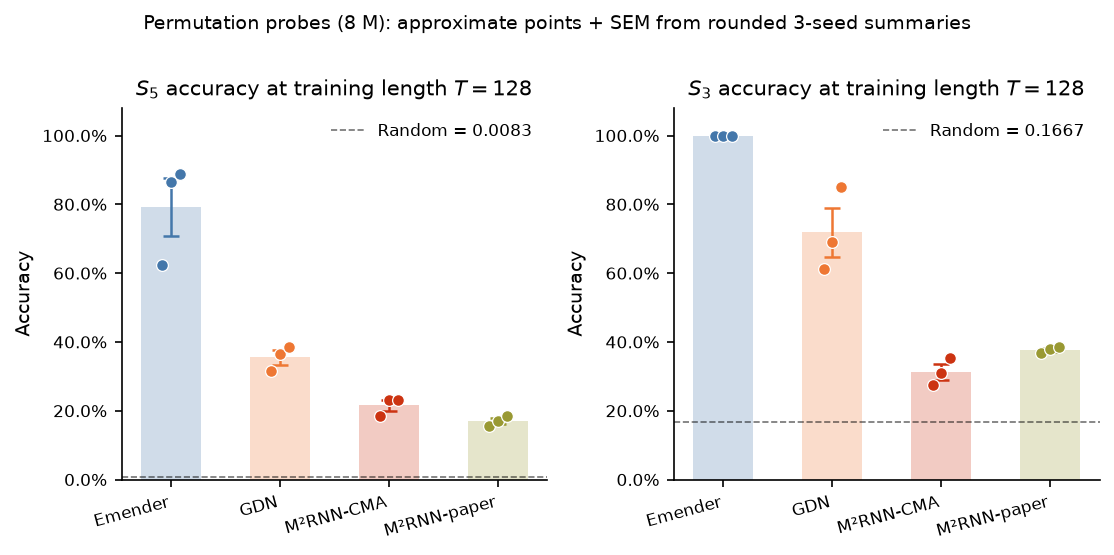
\includegraphics[width=0.95\linewidth]{assets/s5_expressivity_seeds.png}
\caption{ \emph{Expressivity separation on the permutation-composition probes at parameter-matched 8 M scale.} Dots and SEM are approximate reconstructions from rounded three-seed mean/min/max summaries, not retained individual observations. The middle point uses $3 \times  \text{mean} -  \text{min} -  \text{max}$, clamped to the reported min/max interval; SEM is computed from this reconstructed triple. Bars show the reported rounded mean (light fill). The Emender separates from linear-recurrent (GDN) and raw-write nonlinear matrix RNN (M\textsuperscript{2}RNN) baselines on the non-solvable ${S }_{5}$ probe at training length. On the solvable ${S }_{3}$ control, the Emender has rounded mean 1.0000; GDN reaches 0.72; both M\textsuperscript{2}RNN variants stall in the 0.31--0.38 band, indicating that at matched no-tuning budget the raw-write update under-reaches on the prefix-tracking task even on the solvable-group control. Source: \protect\path|paper/ndmpapernotes.md| lines 153--173; figure script: \protect\path|paper/figures/plot_expressivity_seeds.py|. }\label{fig_s5_bars}
\end{figure}


At ${S }_{5}$ training length the Emender reaches 0.79, GDN 0.36, M\textsuperscript{2}RNN-CMA 0.22, M\textsuperscript{2}RNN-paper 0.17. On ${S }_{3}$ the Emender is at 1.00, GDN at 0.72, and both M\textsuperscript{2}RNN variants stall in the 0.31--0.38 band; at matched no-tuning budget the raw-write update under-reaches on the prefix-tracking task even when the group is solvable. The Emender starts at 0.79 at $T  =  128$ and declines to 0.42, 0.22, and 0.11 at $T  =  256$, $512$, $1024$; it climbs higher and falls slower than the baselines but does not reach ceiling at length.

The ${S }_{3}$/${S }_{5}$ split is also where the scope of the M\textsuperscript{2}RNN paper's own state-tracking evaluation matters. Mishra et al. \citep{m2rnn2026}, section 3.2 report length generalization on ${S }_{3}$ alone (a nonabelian \emph{solvable} symmetric group, whose word problem is in TC\textsuperscript{0}) and do not evaluate ${S }_{5}$ or any other non-solvable group. The "perfect state-tracking generalization" framing in that paper does not bear on the NC\textsuperscript{1} regime: at parameter-matched 8 M, the Emender reaches 0.79 on ${S }_{5}$ at training length against the paper-default M\textsuperscript{2}RNN's 0.17.

Algorithm 5 gives the common train/evaluate structure of the probe studies, not a claim that they share one recipe. The 8 M from-scratch studies, successful-seed-conditioned grok curves, and 1.3 B group capacity curriculum retain their own seed sets, stopping rules and trained lengths. The modular-quadratic current-pair protocol is specified separately in Algorithm 6; the capacity OOM outcome below is not replaced by a successful curriculum stage.

\emph{Algorithm 5 --- probe-study train/evaluate loop.}
\begin{verbatim}
Input: arm, seed set, task generator, recorded study recipe
1. For each seed and arm, initialize from scratch or bound weights
   as specified by that study; initialize its optimizer.
2. Generate training batches at the declared trained length(s).
3. Optimize the declared objective until the study's stop rule.
   Record completed stages/updates and any failed stage.
4. For each declared evaluation length, generate held-out batches.
5. Run grad-free forward; count correct predictions on the mask.
6. Save per-seed records; aggregate only the declared seed subset.
Return: accuracy-by-length records and protocol/failure metadata
\end{verbatim}



\subsection*{The six-task canonical sweep}


To verify that the ${S }_{5}$ result is not a single-task artefact we run a six-task canonical sweep covering parity (binary XOR over a stream), modular counter (K=5), FSM tracking (K=4 states), Dyck-1 (balanced brackets), associative recall (key\ensuremath{\rightarrow}value lookup), and selective copy (mark-and-copy). At 8 M parameter-matched scale, the Emender ties or exceeds GDN on five of six tasks (parity 1.00 vs 0.86; modular counter 0.90 vs 0.65; FSM tracking 1.00 vs 0.83; Dyck-1 1.00 vs 1.00; selective copy 1.00 vs 1.00). GDN is ahead of the Emender on associative recall (0.997 vs 0.881), the only attention-natural task in the suite.

Under length extrapolation (train $T  =  40$, evaluate up to $T  =  500$), the Emender retains 0.89 accuracy on parity at $T  =  500$ where GDN collapses to 0.55 (near random 0.50). On FSM tracking at $T  =  500$, the Emender is at 0.59 versus GDN 0.39. The parity gap widens to a peak of about 0.359 at $T  =  320$, then narrows to about 0.337 at $T  =  500$.

Positive gaps persist across the measured lengths for parity, FSM tracking, and modular counter, but they are not monotone: the FSM gap also peaks at $T  =  320$, while the counter gap shrinks throughout. This retained empirical advantage is distinct from the exact finite-$k $ non-equality of Section~\ref{sec:formal} (\protect\path|emender_m2rnn_k_step_separation|, Theorem set C\ensuremath{^{\prime}}) and the one-step resource separation (\protect\path|emender_m2rnn_one_step_resource_separation_embeds|, set C). Neither formal statement predicts an increasing empirical accuracy gap. The remaining frontier, an ${S }_{5}$-generator-specific capacity bound with explicit $T ( d ) $, is named in Section~\ref{sec:future_work}.


\subsection*{Hybrid degradation: purity matters}


A natural question for any architecture that leads on state tracking is whether the gain survives mixing with linear-scan blocks. We test the pattern $[ \text{Emender},  \text{Emender},  \text{GDN},  \text{GDN}] $ (four-layer "AABB" hybrid) on the same canonical sweep and find that \emph{hybridization degrades state tracking below either pure family}:


\begin{figure}[htbp]
\centering
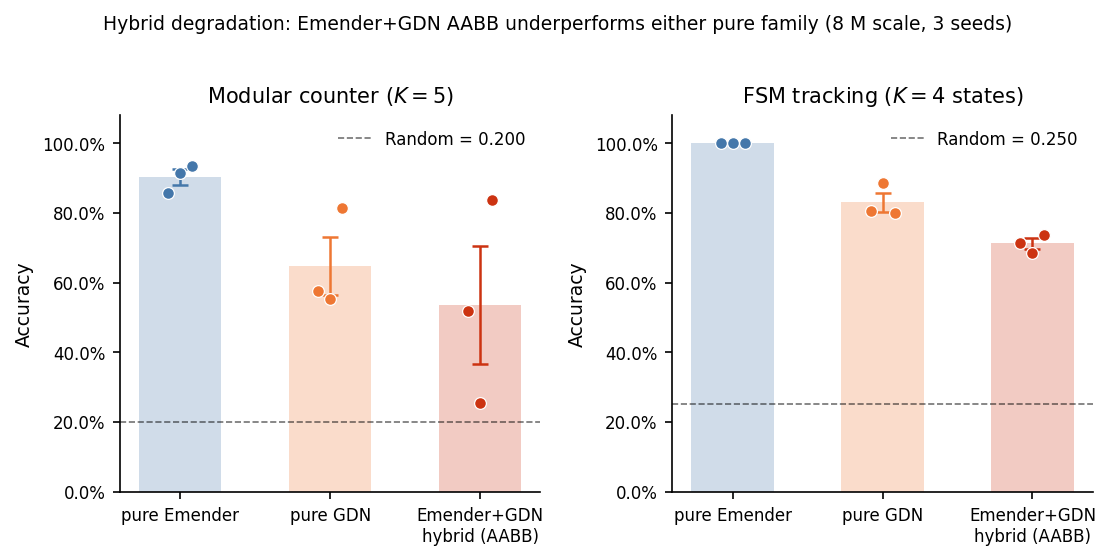
\includegraphics[width=0.95\linewidth]{assets/hybrid_degradation_seeds.png}
\caption{ \emph{Hybrid degradation: per-seed accuracy at 8 M scale, 3 seeds per condition.} Interleaving Emender layers with linear-scan (Gated DeltaNet) layers in an \protect\path|[Emender, Emender, GDN, GDN]| AABB pattern \emph{underperforms} pure Emender on both modular counter ($K = 5$) and FSM tracking ($K = 4$ states), and underperforms pure GDN on modular counter. Bars show the seed mean; error bars span the SEM (standard error of the mean across 3 seeds); individual seed points are overlaid (seeds 42, 123, 456). The dashed line is the random baseline ($\frac{1}{K }$). State-tracking capability is reduced in this tested AABB pairing; Section~\ref{sec:predictions} prediction 5 addresses Emender + attention. Source: per-seed JSON under \protect\path|paper/results/figure_4_hybrid/|; figure script: \protect\path|paper/figures/plot_hybrid_degradation.py|. Mean $\pm $ std mirrors \protect\path|experiments/expressivity_tasks/CANONICAL_SWEEP_RESULTS.md|. }\label{fig_hybrid}
\end{figure}


The hybrid result is the same finding as Section~\ref{sec:arch} from the other side: linear-scan blocks do not inherit state tracking from neighboring Emender blocks.


\subsection*{A controlled update-map ablation on iterated maps}


Before measuring the trained 1.3 B pair, the \emph{mechanism} --- the per-step state nonlinearity --- is tested by a controlled tanh/identity update-map ablation. This does not control every confound in the post-selected seed averages or cross-architecture comparison. On the iterated map ${x }_{t } =  ( {x }_{t - 1}^{2} +  {c }_{t })  \operatorname{mod} p $ with per-position supervision (train length $T  =  128$, evaluate to $T  =  4096$), three arms are trained with width applied \emph{symmetrically} across all of them: \protect\path|e97| (the nonlinear cell), \protect\path|e97-linear| (byte-identical code on the same fused kernel --- the only difference is the per-step state map, $\operatorname{tanh}$ versus identity), and \protect\path|gdn2| (the linear baseline of Section~\ref{sec:lm}'s pairing). Far-length scoring tests transfer beyond the training-length distribution. Length failure is consistent with finite-length heuristics or memorization, but also with approximate recurrence learning and accumulated error; it does not establish algorithm recovery or its absence.

The nonlinear arm is length-invariant where both linear arms collapse: at $p  =  256$, dim 1024, E97 holds $0.982 \rightarrow  0.981$ from $T  =  128$ to $T  =  4096$, while e97-linear falls to 0.619 and GDN2 to 0.560. These source length curves condition on successful training-length seeds (\protect\path|final_test >= 0.9|): 2 E97, 1 e97-linear, and 4 GDN2 seeds in this cell, not an unconditional four-seed mean. Separately, an 8-seed confirmation run puts the E97\ensuremath{-}GDN2 gap at $+ 0.17$ to $+ 0.32$ at $T  =  4096$ across the decisive cells, and the 4-seed symmetric-width sweep shows decisive-cell gaps up to $+ 0.42$ (\protect\path|experiments/grok_symmetric_width/RESULTS.md|, \protect\path|experiments/grok_symmetric_width/CONFIRM.md|). Because \protect\path|e97| and \protect\path|e97-linear| differ by a single flag in the same kernel, the intervention isolates the update map rather than capacity, depth, or kernel choice. The reported successful-seed subsets nevertheless differ, so their conditional curve gap is not an unconditional causal effect estimate or proof of algorithm recovery.

The tested mechanism hypothesis is also probed on two other task families lacking one of its hypothesized conditions; the observed separation is \emph{absent} there. On a contractive logistic map (no long memory to memorize-then-fail), 0 of 24 runs grok and all arms plateau flat across length. On ${a }^{n } {b }^{n } {c }^{n }$ counting (additive accumulation, which linear cumulative state extrapolates as well as bounded nonlinear state), all 24 runs fit and all arms decay together, the gap tiny and sign-flipping. The tested mechanism hypothesis combines repeated non-affine updates with persistent history. The observed negatives support that hypothesis, not a theorem that these conditions are necessary or sufficient for a learned-stack separation. The duality counts the executed updates; it does not lower-bound minimal representation depth (Section~\ref{sec:formal}).


\subsection*{The parameter-matched contractive control}


The pre-registered parameter control closes the historical small-GDN mismatch without changing the task or optimization protocol. On the contractive logistic family, \protect\path|gdn-8m| has 7.94 M parameters versus E97's 7.38 M (7.6\% more, favoring GDN). Its accuracy falls only from 0.896 to 0.854 over the evaluation range (Table~\ref{tab_contractive_control}). The measured mixed-driver Lyapunov exponent is $\lambda  =  \text{\ensuremath{-}0.201} <  0$: this is a contractive control, not a chaotic depth-wall vehicle. Larger parameter count improves the linear arm's accuracy but does not change its mild-decay regime; parameters are not the lever for a compounding wall on this family. Protocol: \protect\path|iterated-map/PLAN.md|, pre-registration \protect\path|0038ad84|; completed control \protect\path|384e657c|.


\begin{table}[htbp]
\centering
\begingroup\setlength{\tabcolsep}{3pt}
\begin{tabularx}{\linewidth}{|>{\hsize=1.71429\hsize\linewidth=\hsize\raggedright\arraybackslash}X|>{\hsize=0.85714\hsize\linewidth=\hsize\raggedright\arraybackslash}X|>{\hsize=0.85714\hsize\linewidth=\hsize\raggedright\arraybackslash}X|>{\hsize=0.85714\hsize\linewidth=\hsize\raggedright\arraybackslash}X|>{\hsize=0.85714\hsize\linewidth=\hsize\raggedright\arraybackslash}X|>{\hsize=0.85714\hsize\linewidth=\hsize\raggedright\arraybackslash}X|}\hline
\emph{Arm} & \emph{Parameters (M)} & \emph{T=128} & \emph{T=256} & \emph{T=512} & \emph{T=1024} \\ \hline
e97 & 7.38 & 0.885 & 0.879 & 0.878 & 0.876 \\ \hline
e97-linear & 7.38 & 0.893 & 0.887 & 0.887 & 0.885 \\ \hline
e97-raw & 7.38 & 0.683 & 0.677 & 0.677 & 0.673 \\ \hline
gdn & 1.60 & 0.869 & 0.857 & 0.847 & 0.822 \\ \hline
gdn-8m & 7.94 & 0.896 & 0.887 & 0.877 & 0.854 \\ \hline
\end{tabularx}
\endgroup

\caption{ \emph{Contractive logistic-map control, from scratch.} Seed-mean accuracy; the historical \protect\path|gdn| row is parameter-mismatched, whereas \protect\path|gdn-8m| has 7.6\% more parameters than E97, conservatively favoring the linear baseline. All arms use the same training/evaluation protocol and 3 seeds. Source: \protect\path|phase1_8m_control_table.json| (commit \protect\path|384e657c|), under \protect\path|paper/results/expressivity_1p3b/iterated-map/|; protocol pre-registered in \protect\path|PLAN.md| (\protect\path|0038ad84|). }\label{tab_contractive_control}
\end{table}



\subsection*{Expressivity at 1.3 B on the trained pair}


The decisive experiment uses the E97 and GDN2-MLP checkpoints of Section~\ref{sec:lm}, with Schedule-Free y-mode recovery, on ${x }_{t } =  ( {x }_{t - 1}^{2} +  {c }_{t })  \operatorname{mod} 256$, 5 input drivers and running supervision. Both arms receive the identical full-fine-tune recipe: bf16 AdamW(betas=0.9,0.95), constant learning rate 0.00005, warmup 300, weight decay 0.01, gradient clip 0.5, batch 32, trained length 128, seed 42. The throughput-derived common cap of 18269 steps was fixed before accuracy was seen (\protect\path|budget.json|, \protect\path|1989656c|). It projects 4.35 GPU-hours of capped training, \emph{not} actual expenditure. The same pre-registered validation-loss plateau rule stopped E97 after 2500 steps and GDN2-MLP after 2200 steps; actual training elapsed 0.649 GPU-hours, excluding loading and final evaluation. Thus this is a common-cap/common-stop-rule comparison, not equal realized training steps or tokens.

The protocol below summarizes the retained driver, \protect\path|scripts/expressivity_1p3b_depthwall.py|, including its zero-based probe indices. It selects the \emph{stop} weights, not the best observed validation checkpoint. The terminal sweep is grad-free and scores every masked position using full-vocabulary argmax; reduced evaluation batches on OOM are recorded rather than interpreted as a new training recipe.

\emph{Algorithm 6 --- matched-cap fine-tune and terminal evaluation.}
\begin{verbatim}
Input: bound y-mode weights; common recipe, cap, seed
1. Build fixed validation batches; initialize AdamW.
2. For step j = 0,...,cap-1:
   a. Draw a batch at T=128; run bf16 forward.
   b. Backpropagate masked cross-entropy over all positions.
      On OOM, split the same batch and accumulate gradients.
   c. Warm up LR for 300 steps, then keep LR constant;
      clip gradient norm to 0.5; take an optimizer step.
   d. Every 100 updates (and at cap), probe validation loss.
      With 4 probes and j >= min(1000,cap), stop if
      loss <= 1e-4 OR both 200/300-step gains are < 1%.
   e. Every 250 updates, record trajectory probes unless stopped.
3. Retain stop weights and actual update count for each arm.
4. For T in {128,256,512,1024,2048,4096,8192}:
   a. Set B=max(1,floor(32768/T)); build 8 seeded batches.
   b. Compute masked accuracy and loss without gradients.
      On OOM, halve B and rebuild with the same length seed.
      If B=1 fails, record an error rather than a score.
Return: training record, stop reason, terminal length sweep
\end{verbatim}


Relative gain divides the loss decrease by the earlier loss magnitude (floored at ${10}^{- 12}$); both trailing windows must pass. The implemented minimum uses the zero-based index $j $, so 1,000 updates alone do not trigger it. The cap, stopping criterion and recipe are common; realized training lengths in updates are not equal.


\begin{table}[htbp]
\centering
\begingroup\setlength{\tabcolsep}{3pt}
\begin{tabularx}{\linewidth}{|>{\hsize=1.60000\hsize\linewidth=\hsize\raggedright\arraybackslash}X|>{\hsize=0.80000\hsize\linewidth=\hsize\raggedright\arraybackslash}X|>{\hsize=0.80000\hsize\linewidth=\hsize\raggedright\arraybackslash}X|>{\hsize=0.80000\hsize\linewidth=\hsize\raggedright\arraybackslash}X|}\hline
\emph{Length} & \emph{Train-length multiple} & \emph{E97} & \emph{GDN2-MLP} \\ \hline
128 & 1\ensuremath{\times} & 99.96\% & 76.09\% \\ \hline
256 & 2\ensuremath{\times} & 99.14\% & 62.85\% \\ \hline
512 & 4\ensuremath{\times} & 90.16\% & 56.55\% \\ \hline
1024 & 8\ensuremath{\times} & 76.07\% & 53.36\% \\ \hline
2048 & 16\ensuremath{\times} & 62.92\% & 51.91\% \\ \hline
4096 & 32\ensuremath{\times} & 55.79\% & 50.74\% \\ \hline
8192 & 64\ensuremath{\times} & 51.79\% & 50.53\% \\ \hline
\end{tabularx}
\endgroup

\caption{ \emph{Modular-quadratic length extrapolation on the released 1.3 B pair.} Full-vocabulary argmax accuracy at the pre-registered plateau stops; trained length 128, seed 42, 262144 scored token positions per length. The identical cap is 18269 steps, not identical realized training: E97 stopped after 2500 steps and GDN2-MLP after 2200. E97 decays gracefully rather than remaining length-invariant; GDN2-MLP approaches a roughly 50\% plateau, \emph{not} the declared 0.39\% random baseline. Source: \protect\path|paper/results/expressivity_1p3b/iterated-map/|, \protect\path|ft_{e97,gdn2}_modular_quadratic{,_sweep}.json| (commit \protect\path|9dc3afd7|); \protect\path|budget.json| (pre-registration \protect\path|1989656c|). }\label{tab_depth_wall}
\end{table}


At the terminal sweep E97 reaches 99.96\% at trained length, retaining 90.16\% at four times and 76.07\% at eight times that length. GDN2-MLP ends at 76.09\% at trained length and 53.36\% at eight times. E97 at eight times approximately matches GDN2-MLP's terminal trained-length accuracy, then decays further; it is not length-invariant. GDN2-MLP approaches a roughly 50\% plateau at the longest lengths, explicitly \emph{not} the declared 0.39\% random baseline. The terminal trained-length value is not a hard ceiling: intermediate GDN2-MLP trajectory probes were higher. One seed, unequal plateau-stop lengths, and validation fluctuations limit the inference; this is the measured modular-quadratic separation under this protocol, not a theorem that the full stack cannot learn the task.

This is the empirical complement to the duality theorems \protect\path|CompositionalDepthDuality.e97_compositional_depth_grows_in_time| and \protect\path|gdn_state_channel_depth_bounded_in_time| (\protect\path|32cfcc9c|): E97 composes one nonlinear state update per time step, whereas the input-only-scheduled GDN state fold remains affine in its initial state, with bounded nonlinear temporal depth. The theorem concerns the state channel, not an impossibility or depth lower bound for a multilayer GDN2-MLP stack. The bridge theorem \protect\path|S5GDNBridge.gdn_s5_realization_requires_per_token_action| (\protect\path|82eec14d|) assumes a token-only schedule and a reachable-state-separating decoder; under those hypotheses the word action factors through ${S }_{5}$ and is affine on the reachable image; a token-independent schedule cannot track it. It is a \emph{routing} theorem, not a per-token circuit-depth lower bound (\protect\path|formal/lean/GAPS-D2.md|). The ${S }_{5}$ results below mark exactly that boundary: an affine state channel does not itself imply failure on group actions.


\subsection*{S5 does not replicate the predicted separation}


The initial suite's negative is retained verbatim: ``The 8M S5 separation does NOT replicate at 1.3B on this pair.'' (\protect\path|paper/results/expressivity_1p3b/SUMMARY.md|, \protect\path|5e1e60ef|). Zero-shot did not separate either model; matched fine-tuning favored E97 on the solvable ${S }_{3}$ control but did not reproduce the small-scale ${S }_{5}$ ordering. The longer-horizon capacity probe and phase-0 salvage confirmed the boundary finding, verbatim: ``in the capacity-exceeded regime on S5 there is no wall for either model --- both decay in parallel toward the random baseline, and GDN2-MLP is ahead of E97 at every length.'' (\protect\path|capacity/SUMMARY.md|, \protect\path|6f916843|).


\begin{table}[htbp]
\centering
\begingroup\setlength{\tabcolsep}{3pt}
\begin{tabularx}{\linewidth}{|>{\hsize=1.50000\hsize\linewidth=\hsize\raggedright\arraybackslash}X|>{\hsize=0.75000\hsize\linewidth=\hsize\raggedright\arraybackslash}X|>{\hsize=0.75000\hsize\linewidth=\hsize\raggedright\arraybackslash}X|}\hline
\emph{Length} & \emph{E97} & \emph{GDN2-MLP} \\ \hline
256 & 0.397 & 0.685 \\ \hline
512* & 0.204 & 0.363 \\ \hline
1024 & 0.109 & 0.190 \\ \hline
2048 & 0.061 & 0.103 \\ \hline
4096 & 0.033 & 0.054 \\ \hline
8192 & 0.021 & 0.034 \\ \hline
\end{tabularx}
\endgroup

\caption{ \emph{S5 capacity/long-horizon boundary finding, not a depth-wall separation.} Full-vocabulary argmax accuracy, seed 42 both curves decay and GDN2-MLP stays ahead. \ensuremath{* }GDN2-MLP completed one optimizer step at length 512 before the curriculum stage proved OOM-infeasible even at sub-batch 1; this point is not wholly untrained. Source: \protect\path|capacity/cap_{e97,gdn2}_s5_sweep.json| and \protect\path|cap_gdn2_s5_train.json| under \protect\path|paper/results/expressivity_1p3b/| (E97 \protect\path|f1ed5615|, GDN2 salvage \protect\path|6f916843|). }\label{tab_s5_boundary}
\end{table}


Both capacity curves decay rather than learn length-invariant tracking; held-out transitions remain weaker than seen ones. GDN2-MLP's attempted length-512 curriculum stage was OOM-infeasible even at sub-batch 1, after one completed optimizer step. This hardware limitation and the single seed remain part of the result, not hidden protocol changes. Neither the bridge nor the duality turns this no-separation finding into an ${S }_{5}$ impossibility. The predecessor cohort's different fine-tune study remains in Section~\ref{sec:appendix_cohort}, not substituted for this pair.


\subsection*{Micro and mega: the two probes bracket the mechanism}


The expressivity claim rests on two complementary measurements that are load-bearing only \emph{together}. The \emph{micro} probe is the 8 M from-scratch sweep (Figure~\ref{fig_s5_bars}, three seeds): it isolates expressivity in the cleanest setting, where the Section~\ref{sec:expressivity} state-count argument gives large storage headroom, so a gap plausibly reflects inductive bias rather than raw state count; its limitation is that an 8 M model is small. The \emph{mega} probe is the completed 1.3 B suite above, on the released E97/GDN2-MLP artifacts the loss-parity claims bind to. The micro probe controls parameter count and seeds; the mega probe controls scale and the trained artifact but supplies only one seed. Together they support a modular-quadratic separation, with graceful rather than invariant E97 extrapolation at 1.3 B, and a negative ${S }_{5}$ transfer. The predecessor cohort's ordering (Section~\ref{sec:appendix_cohort}) cannot override this current-pair boundary finding.


\section{Repeated nonlinear maps in the wild}\label{sec:applications}


The iterated-map probes ask a question that arises well beyond language modeling: can an architecture keep applying a nonlinear transformation to its own evolving state? Consider the broad family
\[\begin{aligned}{S }_{t + 1} =  {F }_{\theta ( {S }_{t }, {u }_{t }) }, \end{aligned}\]
 where $\theta $ is fixed across steps, ${u }_{t }$ injects the current input, and ${F }_{\theta ( \cdot , u ) }$ is generally non-affine in the carried state. A common form is ${S }_{t + 1} =  \varphi ( A ( {u }_{t })  {S }_{t } +  b ( {u }_{t }) ) $; neither an additive injection nor a smooth $\varphi $ is required. Fixed $\theta $ describes the update law, not identical token-dependent coefficients: in the Lean schedule, each step supplies its own key, gates, and value. The formal E97 fold fixes $\lambda $; the architecture additionally supplies input-dependent decay. Autonomous maps have no input injection. The Emender's coupled update
\[\begin{aligned}{S }' =  \operatorname{tanh}( \lambda  S  +  {k ( v  -  {S }^{T } k ) }^{T }) \end{aligned}\]
 is an instance with state $S $, input $( \lambda , k , v ) $, and a fixed delta-correcting $\operatorname{tanh}$ update; it is the all-one split-gate specialization of E97 (Section~\ref{sec:arch}). This is a structural family, not a claim that the systems below share E97's weights, learning rule, or computational difficulty. Algorithm 7 is its time-ordered execution: each returned state is the next step's input. For the abstract E97 fold, the schedule supplies $( k , e , w , v ) $ at fixed $\lambda $; for GDN it additionally supplies $D $ and is independent of the carried state. The application displays below specify ${F }_{\theta }$ and the state/input coordinates for each instance of this same loop.

\emph{Algorithm 7 --- repeated-map fold.}
\begin{verbatim}
Input: initial state S_0, fixed update law F_theta, input schedule
1. S <- S_0
2. For each input u in time order:
   S <- F_theta(S, u)
Return: S
\end{verbatim}


The depth-duality gives a precise lens, but not an application-level lower bound. \protect\path|CompositionalDepthDuality.e97_compositional_depth_grows_in_time| records one additional nonlinear update per time step; \protect\path|gdn_state_channel_depth_bounded_in_time| proves that a GDN state fold is affine in its initial state \emph{conditional on a state-independent input/gate/value schedule}. Neither proves that the resulting function has no shallower representation in other coordinates. The ${S }_{5}$ bridge (\protect\path|S5GDNBridge.gdn_s5_realization_requires_per_token_action|) is a routing statement under its reachable-state-separating decoder hypothesis, not a depth lower bound. It does not transfer a separation to the applications below; group actions can admit affine representations. Here \emph{EXHIBIT} means a definitional or structural instance of the family, \emph{ANALOGY} a related but non-identical mechanism, and \emph{OPEN} a prediction not yet established. In each case the question is whether a fixed-depth GDN-style linear-state approximator can reproduce the required trajectories, not whether the original engineered system already works.


\subsection*{Sigma--delta conversion: quantization inside the loop}


\emph{EXHIBIT.} A first-order sigma--delta modulator accumulates an analog sample and feeds back a quantized output \citep{candy_temes1992}:
\[\begin{aligned}{a }_{t } =  {r }_{t } +  {x }_{t },  \quad  {q }_{t } =  Q ( {a }_{t }) ,  \quad  {r }_{t + 1} =  {a }_{t } -  {q }_{t }. \end{aligned}\]
 Here ${r }_{t }$ is the integrator residue, ${x }_{t }$ the injected sample, and the fixed state map is $F ( r , x )  =  r + x - Q ( r + x ) $. For a one-bit converter, $Q ( a ) $ selects one of two output levels: a hard, discontinuous nonlinearity rather than E97's smooth saturation. The nonlinear result is fed back into the next state, not merely placed in an output readout. Such streaming error-feedback loops are implemented directly in converter circuitry; they need no large learned processor to execute the update. \emph{OPEN:} the duality suggests testing a GDN surrogate near quantizer thresholds over long streams, where residual errors can change later bits. A nonlinear state update represents this feedback directly; a linear residue integrator with an output-only quantizer omits the feedback dependence. No GDN lower bound follows: finite-resolution states, alternative encodings, or a different error metric may make a linear-state surrogate adequate. Predicting filtered signal quality is also weaker than predicting the exact bitstream.


\subsection*{Adaptive filtering and automatic gain control}


\emph{ANALOGY for ordinary normalized LMS; EXHIBIT for the nonlinear variants.} For regressor ${x }_{t }$, desired sample ${d }_{t }$, and coefficient state ${w }_{t }$, normalized LMS \citep{haykin2002} uses
\[\begin{aligned}{e }_{t } =  {d }_{t } -  {w }_{t }^{T } {x }_{t },  \quad  {w }_{t + 1} =  {w }_{t } +  \mu  {x }_{t } \frac{{e }_{t }}{\epsilon  +  {\Vert {x }_{t }\Vert }^{2}}. \end{aligned}\]
 With inputs fixed this is \emph{affine} in ${w }_{t }$: normalization alone is not a nonlinear-state example. A componentwise coefficient-limited variant, ${w }_{t + 1} =  {\text{clip}}_{B ( {w }_{t } +  \mu  {x }_{t } \frac{{e }_{t }}{\epsilon  +  {\Vert {x }_{t }\Vert }^{2}}) }$, is one: state $w $, map the normalized correction followed by clipping, injection $( x , d ) $. The clipping is an additional engineering choice, not part of standard normalized LMS. Automatic gain control similarly feeds the measured output level back into the gain \citep{lyons2011}. A representative bounded log-gain controller is
\[\begin{aligned}{y }_{t } =  \operatorname{exp}( {g }_{t })  {x }_{t },  \quad  {g }_{t + 1} =  {\text{clip}}_{[ {g }_{\operatorname{min}}, {g }_{\operatorname{max}}] } ( {g }_{t } +  \mu ( {P }_{0} -  {y }_{t }^{2}) ) . \end{aligned}\]
 Its state is ${g }_{t }$, its injection is the sample ${x }_{t }$ and target power ${P }_{0}$, and its fixed map includes the state-dependent power measurement and gain limiter. These equations specify representative variants, not universal implementations. \emph{OPEN:} the duality predicts a possible surrogate gap when repeated limiter crossings or gain changes retain consequential history. Ordinary normalized LMS needs no such gap, and a stable AGC loop may forget errors rapidly enough for a linear-state approximation to suffice. These are natural per-sample edge and sensor workloads, but no IoT deployment advantage is measured here.


\subsection*{Proximal iterations and unrolled optimization}


\emph{EXHIBIT.} For the objective $\frac{1}{2} {\Vert A  z - b \Vert }^{2} +  \rho  {\Vert z \Vert }_{1}$, iterative soft-thresholding (ISTA) \citep{daubechies2004} repeatedly applies
\[\begin{aligned}{z }_{j + 1} =  {\text{soft}}_{\eta  \rho } ( ( I  -  \eta  {A }^{T } A )  {z }_{j } +  \eta  {A }^{T } b ) , \end{aligned}\]
 where ${\text{soft}}_{\tau ( a ) } =  \text{sign}( a )  \operatorname{max}( | a | - \tau , 0) $ acts componentwise. The iterate ${z }_{j }$ is the state, the fixed map is a gradient step followed by soft-thresholding, and $\eta  {A }^{T } b $ injects the problem data at every iteration. Here time means optimization iteration, not arriving samples. FISTA \citep{beck_teboulle2009} adds extrapolation,
\[\begin{aligned}{z }_{j + 1} =  {\text{soft}}_{\eta  \rho }( {y }_{j } -  \eta  {A }^{T ( A  {y }_{j }- b ) }) ,  \quad  {y }_{j + 1} =  {z }_{j + 1} +  {\beta }_{j ( {z }_{j + 1}- {z }_{j }) }. \end{aligned}\]
 Its state must include the previous iterate and momentum schedule (or its clock); it is not a single fixed map on ${z }_{j }$ alone. Unrolling these updates exposes their nonlinear depth explicitly; changing weights at every unrolled stage forfeits the fixed-map identification. \emph{OPEN:} the duality predicts difficulty for a fixed-depth linear-state surrogate when support changes must be recomputed over many iterations. It does not say ISTA always requires growing nonlinear depth: after support and signs stabilize, soft-thresholding is affine on the visited region, and convergence can make a bounded-accuracy shortcut sufficient.


\subsection*{Reservoirs and echo-state networks}


\emph{EXHIBIT.} The standard driven echo-state network \citep{jaeger2001} has
\[\begin{aligned}{h }_{t + 1} =  \operatorname{tanh}( W  {h }_{t } +  U  {u }_{t } +  b ) . \end{aligned}\]
 The reservoir state is $h $, the fixed recurrent map is $\operatorname{tanh}$ after mixing by $W $, and the injection is $U  {u }_{t }+ b $. With recurrent parameters held fixed, E97 likewise defines a driven nonlinear dynamical reservoir: its matrix state is mixed, corrected by the input, and passed through $\operatorname{tanh}$ again at each step. \emph{ANALOGY:} it is not the conventional fixed-$W $ echo-state architecture or training protocol. E97's effective state mixing depends on the input key and gates, its recurrent weights are trained, and bounded $\operatorname{tanh}$ state alone does not establish the echo-state property (forgetting the initial condition). \emph{OPEN:} for a reservoir task with persistent nonlinear history the duality motivates comparing E97 with a linear-state surrogate across length. A contractive reservoir instead has fading memory and may admit a good short-history approximation. The structural match does not predict a universal advantage over linear reservoirs with nonlinear readouts, nor establish that E97 satisfies the echo-state property.


\subsection*{Discrete ecology: the logistic map}


\emph{EXHIBIT.} May's population-dynamics example \citep{may1976} is the autonomous logistic map
\[\begin{aligned}{n }_{t + 1} =  r  {n }_{t ( 1- {n }_{t }) }. \end{aligned}\]
 State is normalized population ${n }_{t }$; $r $ is a fixed model parameter; ${F }_{r ( n ) } =  r  n ( 1- n ) $ is applied to its own output with \emph{no} input injection. An environmentally driven variant can supply ${r }_{t }$ as the input, but is then an extension of the autonomous model. This is the same logistic family as the contractive control in Section~\ref{sec:expressivity}, not a claim that its parameter regime represents all ecological dynamics. \emph{OPEN:} the duality motivates a long-horizon surrogate comparison only when nonlinear dependence on prior state remains relevant. The control is the important countercase: contraction suppresses trajectory errors and no depth-wall signature is observed. Periodic attraction can also simplify prediction; chaotic regimes can make precise long-horizon prediction difficult for \emph{both} architectures. Nonlinearity alone therefore cannot imply a separation, and an ecological population equation is not evidence of a deployed forecasting improvement.


\subsection*{Feedback control with limited actuators}


\emph{EXHIBIT.} A discrete-time linear plant with a smooth actuator limit and state feedback can be written
\[\begin{aligned}{a }_{t } =  {a }_{\operatorname{max}} \operatorname{tanh}( \frac{K  {x }_{t } +  L  {r }_{t }}{{a }_{\operatorname{max}}}) ,  \quad  {x }_{t + 1} =  A  {x }_{t } +  B  {a }_{t } +  E  {d }_{t }. \end{aligned}\]
 Here ${x }_{t }$ is plant state; reference ${r }_{t }$ and disturbance ${d }_{t }$ are the injections; the fixed closed-loop map is $F ( x , ( r , d ) )  =  A  x  +  B  {a }_{\operatorname{max}} \operatorname{tanh}( \frac{K  x + L  r }{{a }_{\operatorname{max}}})  +  E  d $. Saturation in feedback is a standard nonlinear-control concern \citep{khalil2002}; $\operatorname{tanh}$ is a smooth bounded-actuator model, not a claim that all actuators implement it. \emph{ANALOGY:} unlike E97, the nonlinearity acts on the control path and the plant state need not be bounded. \emph{OPEN:} the duality predicts a possible linear-state-surrogate deficit when state-dependent saturation repeatedly determines subsequent control decisions. It makes no prediction of a gap in the unsaturated, approximately linear regime, or for a sufficiently contracting closed loop. A learned surrogate would additionally need stability and safety validation; a state-tracking result is not a control guarantee.

These examples make the architecture question concrete. When a workload requires persistent, repeated nonlinear transformation of its carried state, the duality says that nonlinear \emph{state computation} cannot simply be dropped while leaving the same update in the same coordinates: an affine state channel does not perform that operation. In that restricted sense nonlinear-state recurrence is not optional; an alternative must supply an adequate representation or approximation elsewhere. Whether a fixed-depth GDN-style stack can do so at acceptable width, precision, latency, and horizon remains \emph{OPEN} for these applications. Stable, fading-memory and affine-representable cases are explicit exceptions to any blanket advantage claim. The practical opportunity is many small, low-cost, low-intelligence streaming processors operating in parallel at the edge: local feedback and correction rather than a large reasoning model per sensor. Width-axis multi-programming suggests how many such nonlinear programs can coexist without linearizing their internal time loops; low-power silicon, energy savings, and task-level superiority would require separate measurements.


\section{Formal Results}\label{sec:formal}


The claims in this section are checked by a machine rather than argued on paper. A trusted Lean 4 \citep{lean42021} core built on Mathlib \citep{mathlib4} carries the formal spine: each result is stated as a theorem and compiled together with a proof of it. Trust rests on what those proofs are \emph{not} allowed to assume. The import closure of the \protect\path|ElmanProofs.PaperCore| module --- 17 project source files in the recursive local closure --- uses none of Lean's escape hatches: no \protect\path|sorry|, \protect\path|admit|, added \protect\path|axiom|, \protect\path|opaque| declarations, or \protect\path|native_decide|. The gate is \protect\path|formal/lean/scripts/check_paper_core.sh|; compiling \protect\path|ElmanProofs.PaperCore| additionally checks elaboration of the proofs. The refreshed machine-extracted inventory is committed at \protect\path|paper/data/lean-trust-gate-theorems.json| (857 named declarations, 723 user-written, 17 files; extraction source commit \protect\path|e58ae937|), including the split-gated, latching, duality, routing, Lipschitz, and E1H-definition modules. Both the gate and extractor traverse the recursive local imports rather than a selected module allowlist. This check covers project sources, not the axioms or source files of Lean and Mathlib dependencies.

Every result below is named by its exact theorem so a reader can open the source and find it. What is proved here is realizability and representational scope; what a trained model actually learns under SGD is the separate empirical question of Section~\ref{sec:lm} and Section~\ref{sec:expressivity}.

The formal spine starts with the compositional-depth duality and routing bridge (set H below), which explain the lens used in Section~\ref{sec:expressivity} and Section~\ref{sec:formal}. The remaining sets specify exact lookup, recognizer count, matched-signature update separation, resource cost, and conditional latching. Exact non-equality on a constructed real-valued witness is not a uniform error margin, and table lookup is not recurrent $\operatorname{tanh}$-tracker realizability.


\subsection*{Theorem set A: finite-state ceiling and ${S }_{5}$ tracker}


\emph{What to take from set A: at fixed width and precision the Emender is a finite-state machine, and the ${S }_{5}$ word problem it is tested on is a concrete, fully specified finite-state target.}


\begin{theorembullet}
\emph{Finite-state ceiling at fixed precision.} At fixed width and precision, every online recognizer of this kind has only finitely many distinct states (\protect\path|S5Witness.fixed_precision_state_space_finite|). This bounds its online memory to finitely many states; it does not prove strict containment below NC\textsuperscript{1}.
\end{theorembullet}
\begin{theorembullet}
\emph{${S }_{5}$ word problem.} The target is pinned down exactly in Lean. The group ${S }_{5}$ has 120 elements (\protect\path|S5Witness.s5_state_count|) and is non-solvable (\protect\path|S5Witness.s5_not_solvable|); the prefix-product tracker that reads a word of transpositions and reports the running product is a 120-state recognizer (\protect\path|S5Tracker.recognizer_state_count|) whose state composes correctly as tokens are appended (\protect\path|S5Tracker.run_append|). A bridge lemma confirms the Lean tracker agrees with the Python evaluation harness on every input (\protect\path|S5Tracker.pythonRun_eq_tracker_tuple|). The four adjacent transpositions generate all of ${S }_{5}$: the tracker's run map is surjective (\protect\path|S5Inseparability.run_surjective|, via Mathlib's \protect\path|Equiv.Perm.mclosure_swap_castSucc_succ|).
\end{theorembullet}
\begin{theorembullet}
\emph{Capacity lower bound (recognizer floor).} Any finite-state recognizer with a state decoder that reproduces the tracker on every input word needs at least 120 states (\protect\path|S5Inseparability.capacity_lower_bound_120|); equivalently, no recognizer with fewer than 120 states can realize it under any decoder (\protect\path|S5Inseparability.small_recognizer_cannot_realize_s5|). The bound has a distinguishing-pair form: any recognizer with too few states admits two words it cannot tell apart that the tracker does distinguish (\protect\path|S5Inseparability.exists_distinguishing_word_pair|). This is the existential form of the ${S }_{5}$-coset inseparability target: it holds for \emph{any} finite recognizer family, with no architectural assumptions, and it is the load-bearing state-counting lemma any future bounded-precision raw-write bound must land against.
\end{theorembullet}
\begin{theorembullet}
\emph{Lookup-table realization.} The tracker is small enough to write down as a table: it uses exactly $120 \times  4 =  480$ state/input keys (\protect\path|S5NDMRealization.s5_transition_key_count|), and any finite recognizer admits such an exact lookup-table realization (\protect\path|S5NDMRealization.exactTransitionMemory_run|).
\end{theorembullet}

\subsection*{Theorem set B: generator-table lookup, not a recurrent tracker}



\begin{theorem}
The exact statement of \protect\path|NDMRealizesS5.emender_realizes_s5_tracker| supplies $d = 12$, four orthonormal keys and one-hot values, queries, a decoder, and $\lambda = 1$. Reading a \emph{preloaded} table retrieves the current generator; decoding it and \emph{externally multiplying a supplied} ${S }_{5}$ state $s $ reproduces the transition $s  \cdot  g $. The linear readout retrieves a generator value, not the running product. The supporting \protect\path|OnlineMemory.linearDeltaWrite_overwrites_one_preserves_others| is an exact \emph{pre-$\operatorname{tanh}$} overwrite statement. Neither theorem states that iterating the nonlinear cell from zero tracks every input word.
\end{theorem}


\emph{Open item F1 --- recurrent $\operatorname{tanh}$-tracker realization unavailable.} The loaded generator memory does not carry the running group product; external composition supplies the missing state computation. Closing F1 requires a configuration of the actual nonlinear update, an explicit initial state and decoder, and an all-words trajectory theorem. This is not a missing proof of the already-proved lookup identity, but a stronger, currently unproved architecture claim.


\subsection*{Theorem set C: update-family separation}


\emph{What to take from set C: in a single step the delta-correcting write does something no fixed-weight raw-write update of the matched shape can reproduce on the abstract witness domain.}

The Emender's delta-correcting write and M\textsuperscript{2}RNN's raw outer-product write are provably distinct as update families over unrestricted real-valued keys, values, and states. The mixed key is $( 1, 1) $ (not unit-normalized), and the prescribed initial state is nonzero. These witnesses are not production zero-state trajectories with normalized keys and finite-logit sigmoid gates, nor full-network separation under arbitrary reparameterization.


\begin{theorembullet}
\emph{Mechanism separation.} The delta write exactly overwrites the addressed slot while leaving every orthogonal query untouched (\protect\path|OnlineMemory.linearDeltaWrite_overwrites_one_preserves_others|), whereas the raw outer-product write cannot satisfy that uniform one-step overwrite specification (\protect\path|OnlineMemory.rawOuterWrite_not_uniformOneStepOverwrite|).
\end{theorembullet}
\begin{theorembullet}
\emph{One-step resource separation.} For every $K  \geq  2$ and $V  \geq  1$, no fixed-weight M\textsuperscript{2}RNN parameterization with row, column, or cell forget gates can match the Emender's mixed-key delta correction in a single recurrent step (\protect\path|RecurrentResourceFormalism.emender_m2rnn_one_step_resource_separation_embeds|). The result is sharp: it covers every external-forget shape the M\textsuperscript{2}RNN signature allows.
\end{theorembullet}
\begin{theorembullet}
\emph{Positive embedding.} The separation is about resources, not raw capability. \emph{Given} the extra read-then-delta resource, M\textsuperscript{2}RNN can embed one Emender step (\protect\path|M2RNNComparison.m2rnn_read_then_delta_embeds_e88_delta_update|); the previous bullet says that without that extra resource it cannot.
\end{theorembullet}

\subsection*{Theorem set C\ensuremath{^{\prime}}: multi-step (k-step) separation}


\emph{What to take from set C\ensuremath{^{\prime}}: the one-step gap does not average out under composition --- it persists at every length on a constructed input.}

The one-step separation persists as exact non-equality at each finite length, not as a length-independent accuracy margin.


\begin{theorem}
 \emph{For every $k  \geq  1$, there is an explicit $k $-token input sequence such that the $k $-step trajectory of any fixed-weight raw-write resource (in the row/column/cell external-forget class) diverges from the Emender's $k $-step trajectory by a nonzero entry for each finite $k $ (Lean: \protect\path|emender_m2rnn_k_step_separation|).}
\end{theorem}


The witness alphabet is the 2-dimensional construction from set C followed by zero-input filler tokens (\protect\path|kStepWitnessInputs k = (mixedKey, 0) :: zeroSteps (k - 1)|). It starts from the prescribed nonzero \protect\path|lowerLeftState|, with unnormalized key $( 1, 1) $ and zero-key fillers. Like set C, set C\ensuremath{^{\prime}} is over an unrestricted abstract real-valued signature, not the production normalized-key, zero-initial-state domain. The proof inducts on the tail, using a lemma that keeps entry $( 0,  0) $ pinned at zero on the raw-write side for every $k $ (\protect\path|FixedRightRawExternalForget2_preserves_zero_row|), while the Emender side reduces to the $k $-fold composition of $\operatorname{tanh}$ at $- 1$, which is nonzero because $\operatorname{tanh}$ is injective. Its magnitude need not stay bounded away from zero as $k $ grows; the statement uses exact real arithmetic. A second form of the theorem packages the same statement existentially over $k $-step input sequences (\protect\path|emender_m2rnn_k_step_separation_exists|), and the two-step case is exposed separately as the inductive base (\protect\path|emender_m2rnn_two_step_separation|). All three live in \protect\path|ElmanProofs.Architectures.MultiStepSeparation|, part of the trusted import closure of \protect\path|PaperCore|. The Section~\ref{sec:expressivity} length-extrapolation curves retain positive, non-monotone gaps on parity, FSM tracking, and modular counter. The parity gap peaks near 0.359 at $T  =  320$ before narrowing to about 0.337 at $T  =  500$. These measurements are separate evidence of retained advantage, not consequences of the exact-real finite-$k $ theorem or an increasing-gap prediction.


\subsection*{Frontier and unproven targets}


\emph{What to take from this: the clean k-step result is the ceiling reachable by direct composition; the }existential\emph{ form of the ${S }_{5}$ capacity inseparability is now proved (set A), and what remains open is the bounded-precision raw-write form with an explicit $T ( d ) $.}

The k-step separation above is the \emph{clean ceiling reachable from the one-step proof by direct composition}. The scope of what it does and does not establish is named below, before stating Theorem set D.


\begin{itemize}
\item \emph{What is proved.} k-step trajectory separation on a constructed 2D input alphabet, for every $k  \geq  1$ and every resource in the row/column/cell external-forget class (\protect\path|emender_m2rnn_k_step_separation|). The outputs differ at every finite $k $ on this alphabet; no compounding or uniform margin is proved.
\item \emph{What is now also proved (set A).} The \emph{existential} capacity form of the ${S }_{5}$ inseparability target: no finite recognizer with fewer than 120 states realizes the tracker, for any architecture (\protect\path|S5Inseparability.capacity_lower_bound_120|), together with generator surjectivity (\protect\path|run_surjective|). Two items that earlier drafts of this section listed as open --- adjacent-transposition generation of ${S }_{5}$, and a state-counting lower bound --- are closed by these theorems.
\item \emph{What is still not proved.} That the gap compounds \emph{on the ${S }_{5}$ generator alphabet specifically} against the raw-write resource class with an explicit length bound $T ( d ) $, i.e., a statement of the form "for any fixed-weight raw-write RNN at state dimension $d $ there is an explicit $T ( d ) $ past which ${S }_{5}$ coset tracking is unreachable, while the Emender at the same $d $ tracks it". That is the stronger inseparability claim; the trusted Lean core does not contain it, and the empirical sections stand in for it.
\item \emph{Why the stronger claim is not in the trusted core.} The remaining form is a \emph{capacity-over-continuous-state} statement: the raw-write class is parameterised by continuous-valued matrices and vectors, so the finite recognizer argument of set A does not directly apply. It requires a bounded-precision discretization (Liu et al.-style fixed-point weights and activations) or a direct trajectory-distinguishability counting argument, plus Merrill-style state-counting machinery in the style of Merrill, Petty and Sabharwal \citep{merrill2024transformers}. Mathlib does not currently provide NC\textsuperscript{1} / TC\textsuperscript{0} circuit classes, finite-state-tracking lower bounds for parameter-bounded RNNs, or pigeonhole capacity arguments specialized to recurrent maps with bounded weight matrices. Each piece is a research-grade mechanization project in its own right; the integration is what would close the gap. The set A bound is the load-bearing state-counting lemma any such argument must land against.
\item \emph{Connection to the empirical claim.} The ${S }_{5}$ accuracy curves of Section~\ref{sec:expressivity} (Figure~\ref{fig_s5_bars}, Table~\ref{tab_s5}) and the canonical-sweep length-extrapolation curves are the \emph{empirical} evidence for the stronger claim that the formal core does not yet reach. Section~\ref{sec:formal} proves finite-$k $ non-equality on a constructed witness; Section~\ref{sec:expressivity} measures finite-length learning behavior on the ${S }_{5}$ generators, not the stronger $T ( d ) $ impossibility.
\end{itemize}
The full status of this push, including what bridging machinery would be required (bounded-precision raw-write class, reachable-state counting, Merrill-style capacity lemma), is documented in \protect\path|formal/lean/LEAN_FRONTIER.md|.


\subsection*{Theorem set D: synthetic state-pass cost class}


\emph{What to take from set D: the updates share a quadratic envelope in a coarse state-pass accounting model, not a verified actual FLOP count.}


\begin{theorem}
\protect\path|RecurrentResourceFormalism.emender_m2rnn_flop_class_equiv| bounds the declared six/seven-state-pass charges by a common ${c }_{1} {d }^{2} +  {c }_{2} d $ form. This synthetic model excludes the actual dense right-multiplication $H  W $ and feature-network costs. An arbitrary dense square $H  W $ has cubic arithmetic cost, whereas the model charges one state-sized atom. Thus this theorem does not certify actual matched empirical compute or explain away implementation-level cost differences.
\end{theorem}



\begin{theorem}
The separately valid E97-versus-E88 result uses the stated \emph{precomputed-gate recurrent-update accounting model}: at matched square state dimension the heads share the same leading ${d }^{2}$ charge (\protect\path|e97_e88_same_leading_per_head_recurrent_cost|), and with gate applications counted separately, for $d  \geq  2$ E97 is bounded by $7 {d }^{2}$ where E88 is $6 {d }^{2}$ (\protect\path|e97_precomputed_gates_same_quadratic_cost_class_as_e88|). This excludes gate/feature-network computation and carries no empirical efficiency claim.
\end{theorem}



\subsection*{Resource scope, not a parameter-efficiency lower bound}


Set C proves nonrepresentability at the specified update signature; set D supplies only a shared synthetic state-pass envelope. Neither shows how many extra parameters would suffice, or that extra state is the only remedy: \protect\path|M2RNNComparison.m2rnn_read_then_delta_embeds_e88_delta_update| supplies a different resource, the missing read-then-delta operation. No minimal parameter-count corollary is claimed.


\subsection*{Theorem set E: multi-programming as a structural predicate}


\emph{What to take from set E: a simple signature-field predicate is shared by E88 and a declared M\textsuperscript{2}RNN proxy, not a kernel concurrency certificate.}


\begin{definition}
The predicate \protect\path|IsMultiProgrammed| requires four declared fields: at least two heads per layer, positive state scalars per head, a pure recurrent stack, and \protect\path|sequentialManyProgram| implementation mode. \protect\path|RecurrentResourceFormalism.multiProgrammed_admits_m2rnn_and_emender| proves it for \protect\path|e88NDM_1p27B| and \protect\path|m2rnnCMAShape = m2rnnPure 22 70 256|. That M\textsuperscript{2}RNN instance is a CMA-representative proxy, not the trained 1.3 B predecessor (depth 21, $H  =  370$, $N  =  16$, hence 256 state scalars/head). The trained geometry meets the same field conditions by inspection/arithmetic. The predicate does not verify kernel scheduling, per-batch independence, or concurrent execution across layers; its class-level meaning is limited to these declared signature conditions.
\end{definition}



\subsection*{Theorem set G: the split-gated update --- E97, E88, and GDN-2}


\emph{What to take from set G: over abstract real-valued gate/key/state signatures, E97 extends E88; GDN-2 has an adjacent scan-compatible linear core with different decay placement. This is not a whole-stack production inclusion theorem for the Section~\ref{sec:lm} pairing.}

The E97 split-gated update is defined in Lean alongside the E88 coupled update, and the module \protect\path|SplitGatedDelta| in the refreshed inventory proves the structural relations the body relies on:


\begin{theorembullet}
\emph{E97 extends E88 in the abstract gate domain.} With both split gates fixed to one, the E97 update specializes exactly to the E88 update, in both direct and expanded form (\protect\path|e97_specializes_to_e88_all_one_gates_direct|, \protect\path|e97_specializes_to_e88_all_one_gates_expanded|), so E97 weakly generalizes E88 (\protect\path|e97_expresses_e88_by_specialization|). The E88 parameterization is therefore a developmental special case, not a rival in this abstract domain. Exact all-one gates are limiting values, not finite-logit production sigmoid outputs.
\end{theorembullet}
\begin{theorembullet}
\emph{The extension is strict on an abstract concrete witness.} E97 realizes a 2-dimensional split erase/write transition with non-parallel write and erase directions (\protect\path|e97_realizes_splitWitness_transition|) that \emph{no} E88 coupled transition can realize (\protect\path|e88_cannot_realize_splitWitness_transition|; the witness directions are non-parallel by \protect\path|splitWitness_dirs_not_parallel|), and a 1\ensuremath{\times}1 zero-state witness separates the strict-gate E97 update from every all-one-gate E88 setting on the same state/input (\protect\path|e97_split_gate_strict_witness_not_e88_all_one|). The 2D witness uses key $( 1, 1) $ and erase gate $( 1, 0) $ and compares transition factors, not arbitrary reparameterized full-network functions. The 1\ensuremath{\times}1 witness uses write gate \emph{2}, outside the production sigmoid range $( 0, 1) $; it does not demonstrate production-gate expressivity.
\end{theorembullet}
\begin{theorembullet}
\emph{Adjacent split-gated cores with different decay placement.} The GDN-2 linear core is the E97 linear core applied to a pre-decayed state (\protect\path|gdn2LinearCore_eq_e97LinearCore_on_decayed_state|), and under identity decay the two coincide (\protect\path|gdn2LinearCore_identity_decay_eq_e97LinearCore_one|); the resource signatures then split exactly on the axis the paper tests empirically: E97 has matrix state, full-state temporal nonlinearity, delta writes, and no scan-compatible state path (\protect\path|e97_split_gated_resource_signature_like_e88|), while the GDN-2-style split erase/write resource has matrix state and delta-style writes but \emph{no} temporal state nonlinearity and a scan-compatible linear state (\protect\path|gdn2_split_erase_write_is_scan_compatible_linear_state|).
\end{theorembullet}
The Section~\ref{sec:lm} pairing is thus anchored on both sides: the two 1.3 B arms share adjacent split-gated delta cores and differ on the per-step state nonlinearity and decay placement, as well as geometry and input processing in the trained stacks --- the same state-map axis the Section~\ref{sec:expressivity} iterated-map ablation isolates as an update-map intervention (\protect\path|e97| versus \protect\path|e97-linear|), distinct from the post-selected curve comparison, and the same axis set G names formally.


\subsection*{Theorem set F: latching}


\emph{What to take from set F: conditional slot-level saturation, hold, and release bounds, not production-default persistent binding.}

These three results formalize the latching half of the Emender primitive: saturation makes a slot insensitive to further bounded writes, sign is preserved under sub-threshold counter-input, and a sufficient counter-delta releases the latch. All three are slot-wise statements on the full abstract Emender update, where $v $ denotes the bounded post-nonlinearity value input already supplied to the recurrent body, ${S }' =  \operatorname{tanh}( \lambda  S  +  k  {( v  -  {S }^{T } k ) }^{T }) $ at slot $( i , j ) $, with $\omega  :=  {k }_{i } ( {v }_{j } -  {( {S }^{T } k ) }_{j }) $ the write contribution into that slot. The proofs run through the standard tanh-perturbation foundation. The module carrying them (\protect\path|EmenderLatching|, introduced at \protect\path|696299b4|) is included in the refreshed inventory and the current clean \protect\path|lake build ElmanProofs.PaperCore|.


\begin{theorembullet}
\emph{Saturation insensitivity.} If the slot is saturated in the sense $| {{S }'_{i , j }}|  >  1 -  \epsilon $, and a perturbation $\delta $ to the pre-activation entry has $| \delta |  \leq  M $ with $\epsilon  +  M  <  1$, then the post-tanh slot moves by at most $2( \epsilon  +  M )  | \delta | $. The bound shrinks linearly in both the saturation slack $\epsilon $ and the perturbation magnitude $M $; at deep saturation a bounded write barely moves the slot. Lean: \protect\path|EmenderLatching.emender_saturation_insensitivity|. A two-input corollary \protect\path|EmenderLatching.emender_saturation_two_inputs_close| lifts the bound to two value vectors sharing one key.
\end{theorembullet}
\begin{theorembullet}
\emph{Sign-preserving hold.} With $\lambda  \geq  1$ and a bounded write $| \omega |  \leq  T  <  \lambda  ( 1 -  \eta ) $ at slot $( i , j ) $, a slot already saturated with $| {S }_{i , j }|  >  1 -  \eta $ keeps its sign after one Emender step and stays bounded below in magnitude by $\operatorname{tanh}( \lambda  ( 1 -  \eta )  -  T ) $. For $\lambda  >  1$ and small $\eta ,  T $ the argument $\lambda  ( 1 -  \eta )  -  T $ exceeds $1$, so the lower bound exceeds $\operatorname{tanh} 1 \approx  0.76$ and the latch holds with margin. The hypothesis $T  <  \lambda  ( 1 -  \eta ) $ is the "no sufficient counter-delta" clause; counter-delta release is the next result. Lean: \protect\path|EmenderLatching.emender_latch_holds_by_default|.
\end{theorembullet}
\begin{theorembullet}
\emph{Counter-delta release.} With $\lambda  >  0$, ${S }_{i , j } >  0$, and a write contribution $\omega  <  - \lambda  {S }_{i , j }$ in the opposite sign, the post-update slot is strictly negative --- the latch flips out of its basin in one step. Symmetrically for the negative basin. The release threshold is ${T }^{\ast } :=  \lambda  | {S }_{i , j }| $; any counter-delta exceeding ${T }^{\ast }$ in the opposite sign suffices. Lean: \protect\path|EmenderLatching.emender_latch_releases_on_counter_delta|. The quantitative companion \protect\path|EmenderLatching.emender_latch_release_quantitative| shows that if the counter-delta exceeds the threshold by margin $\mu  >  0$, the post-update slot lies on the opposite side of the origin with magnitude at least $\operatorname{tanh} \mu $.
\end{theorembullet}

\subsection*{Theorem set H: compositional-depth duality and routing}



\begin{theorem}
The concrete repeated-map family is the schedule of \protect\path|CompositionalDepthDuality.E97Step| values $( k , e , w , v ) $ at fixed $\lambda $ (Lean field \protect\path|b| is the paper's erase gate $e $), acting through \protect\path|e97Step| on matrix state. \protect\path|e97Step_eq_tanh_comp| identifies the step as elementwise $\operatorname{tanh}$ after the state-affine split-gated core. \protect\path|e97StateAfter_eq_compose| gives its time-ordered composition, and \protect\path|e97_compositional_depth_grows_in_time| states that appending a step applies one more such map. Thus the \emph{executed} composition contains one $\operatorname{tanh}$ per token. This is not a proof that the resulting function has no shallower representation.
\end{theorem}



\begin{theorem}
For a fixed, state-independent schedule of \protect\path|CompositionalDepthDuality.GdnStepParams|, \protect\path|gdn_state_channel_depth_bounded_in_time| gives matrices $A , C $ with ${S }_{T }= A  {S }_{0}+ C $ for every initial state (Lean writes $H $ for this matrix, not the head count or the M\textsuperscript{2}RNN comparator state). The nonlinear temporal depth of that \emph{state channel} is zero; a multilayer GDN2-MLP stack, state-dependent gates, approximation error, and alternative encodings are not covered.
\end{theorem}



\begin{theorem}
\protect\path|S5GDNBridge.gdn_s5_realization_requires_per_token_action| assumes a token-only schedule and a decoder that recovers \protect\path|S5Tracker.run| on every word and separates reachable states. It then gives a state map $F $ through the group element, with affine word actions implementing right multiplication on the reachable image. \protect\path|gdn_s5_constant_parameters_cannot_realize| rules out a token-independent schedule. The bridge locates token-dependent actions; it does not rule out affine group representations or lower-bound the network generating their parameters. G1--G3 (Section~\ref{sec:limitations}) record those gaps.
\end{theorem}



\subsection*{Complexity statements and explicit non-claims}


\emph{Lean-proved:} finite-state memory at fixed precision (\protect\path|S5Witness.fixed_precision_state_space_finite|), a non-solvable 120-element group (\protect\path|s5_not_solvable|, \protect\path|s5_state_count|), the exact abstract tracker, the recognizer floor (\protect\path|S5Inseparability.capacity_lower_bound_120|), and the generator-table lookup of set B. Full recurrent $\operatorname{tanh}$-tracker realization is F1, not a theorem. \emph{Cited, not formalized here:} Barrington's NC\textsuperscript{1} completeness result \citep{barrington1986} and circuit containments for restricted SSMs and transformers under their respective arithmetic assumptions \citep{merrill2024transformers} \citep{merrill_sabharwal2023log_precision} \citep{chiang2025uniform_tc0}. No strict separation of TC\textsuperscript{0} and NC\textsuperscript{1} is known or assumed here.

The core proves neither a families-wide linear-scan ${S }_{5}$ impossibility, Barrington's theorem, a per-token circuit-size/depth lower bound, learned weight recovery of a recurrent tracker, nor the raw-write ${S }_{5}$-generator-specific $T ( d ) $ target. Exact finite-$k $ non-equality is not robustness at finite precision. Latching also remains conditional: the hold theorem assumes $\lambda  \geq  1$, whereas production decay is below one, so it is not a default persistence guarantee for the trained E97. These are the boundaries that the empirical and applications sections retain.


\section{Related Work}\label{sec:related}



\subsection*{Ancestry: the fast-weight line on delta correction}


The Emender update belongs to a long line that treats memory as a structure to correct rather than to refill. The earliest formulation is Widrow and Hoff's least-mean-square rule \citep{widrow_hoff_1960}, which writes the error between target and current output back into the weight vector of an adaptive linear element. Schmidhuber recast the same idea in a recurrent setting under the name \emph{fast-weight programmers} \citep{schmidhuber_1992_fastweights}: a slow controller emits keys and values that update a fast-weight matrix online, with the update being a correction against what the matrix currently predicts at the addressed slot. Schlag, Irie, and Schmidhuber made the bridge to modern attention explicit \citep{schlag_irie_schmidhuber_2021}, showing that linear-transformer kernels with cumulative outer-product updates \emph{are} fast-weight programmers with a raw additive write, and proposing the delta-rule write as a stability and capacity fix. DeltaNet \citep{deltanet2024} carried the delta rule into a parallelizable linear-recurrent language model, demonstrating the rule at billion-parameter scale in the linear-state regime. The Emender extends this line with three properties the linear instantiations forfeit: a nonlinear matrix state, the saturation latching of Section~\ref{sec:arch} ingredient (c), which motivates persistent binding under the conditional slot-level hold result ($\lambda  \geq  1$ plus a write budget), not an achieved production-default property; and width-axis parallelism via multi-programming that recovers throughput without time-axis linearization.


\subsection*{Linear-state recurrent language models}


The dominant comparison cohort is the family of linear-state billion-parameter recurrent LMs surveyed in Section~\ref{sec:background}: Mamba \citep{mamba2024} and Mamba2 \citep{mamba2_2024} (selective SSMs); RetNet \citep{retnet2023} (decayed linear attention); GLA \citep{gla2023} (gated linear attention); DeltaNet \citep{deltanet2024} (delta rule, linear in $S $); Gated DeltaNet \citep{gated_deltanet2024} (gated delta rule); RWKV-4/5/6/7 \citep{rwkv4_2023} \citep{rwkv7_2025} (linear-state WKV / generalized delta rule with linear state); HGRN2 \citep{hgrn2_2024} (gated linear RNN with state expansion); MinGRU/MinLSTM \citep{mingru_2024} (input-only gates, linear scan); mLSTM/xLSTM-7B \citep{xlstm7b2025} (covariance update); Griffin/RecurrentGemma \citep{griffin2024} (RG-LRU, often hybridized with local attention). Circuit-containment results for restricted SSM families require their stated transition and arithmetic assumptions \citep{merrill2024transformers}; affinity alone is not a universal complexity classification. The empirical panel in Section~\ref{sec:expressivity} directly tests Gated DeltaNet as the matched representative of this cohort and observes ${S }_{5}$ collapse at length.

In the broader SSM/sequence-model lineage, S5 \citep{s5_2022} introduces simplified state-space layers with a multi-input multi-output linear state-space recurrence. It is distinct from the permutation group ${S }_{5}$ used as a probe here; the cited S5 results concern sequence models, not billion-parameter recurrent LMs.

A newer linear-state result, Gated DeltaNet-2 \citep{gated_deltanet2_2026}, decouples channel-wise erase and write gates and is reported by its authors to outperform GDN. It extends retrieval and state-tracking behavior inside the linear-state envelope, and it is the linear-recurrent baseline of this paper's 1.3 B pairing: the GDN2-MLP arm of Section~\ref{sec:lm} is the official-style Gated DeltaNet-2 mixer (external source commit \protect\path|95709fc|) with the same SwiGLU MLP as E97, selected by the same CMA-ES protocol. The E97 split gates of Section~\ref{sec:arch} are the Emender's corresponding edit --- key-axis erase/read plus value-axis write --- inside a \emph{nonlinear} state map, so the two architectures are adjacent by design (Section~\ref{sec:formal}, set G) rather than by coincidence. Its decoupled gates are a natural next ablation for the multi-programmed substrate, being the kind of bounded per-step-body variant that does not require a new time-parallel scan.


\subsection*{Pure-nonlinear-recurrent peers and adjacent nonlinear-state work}


\emph{M\textsuperscript{2}RNN} \citep{m2rnn2026} (Mishra, Tan, Stoica, Gonzalez, Dao 2026) introduces nonlinear matrix-state recurrence with a raw-write update $Z  =  \operatorname{tanh}( H  W  +  k  {v }^{T }) $. It shares the central systems premise of this work --- that a nonlinear recurrence is serial in time and must take its parallelism from the batch and head axes --- and demonstrates that the update trains at 410 M dense and 7 B MoE scale on Nemotron-CC-v2. Its headline demonstrations and promoted deployment recipe, however, use the nonlinear-matrix-recurrent layer \emph{sparingly inside hybrid stacks} (interleaved with attention layers), and its paper-default pure shape diverged as a pure recurrent backbone at 1.3 B in our setup (Section~\ref{sec:appendix_cohort}). Under the addressing-bottleneck hypothesis, shared-address concentration may contribute, but the reshape also changes width, depth, and head count. Our M\textsuperscript{2}RNN-CMA comparator, used as a within-class baseline at the 8 M probes of Section~\ref{sec:expressivity} and in the Lean separation of Section~\ref{sec:formal}, is therefore not a strawman: it is the same raw-write family after CMA-ES has moved it into the stable, pure-recurrent, address-program-multiplexed regime --- the \emph{pure-recurrent variant} of M\textsuperscript{2}RNN's architecture with no attention layers, CMA-tuned to restore stable training at 1.3 B. The contribution of this work relative to M\textsuperscript{2}RNN is to extend the viability demonstration to that \emph{pure-recurrent} setting and to add the direct comparison with the Emender under matched per-architecture CMA-ES. In the predecessor-cohort regime (Section~\ref{sec:appendix_cohort}) the raw-write model was descriptively close to the Emender on held-out language-modeling bpb but remained behind on ${S }_{3}$/${S }_{5}$ tracking. The empirical comparison in Section~\ref{sec:expressivity} controls the broad pure-recurrent systems setting for comparing the \emph{write rule} --- delta-correcting (the Emender) versus raw-write (M\textsuperscript{2}RNN-CMA) --- without uniquely isolating a causal mechanism; the formal one-step resource separation in Section~\ref{sec:formal} applies under its declared accounting model. Mishra et al. also report hybrid M\textsuperscript{2}RNN configurations favorably against Mamba2 and Gated DeltaNet hybrids at matched parameter and token budgets under a uniform fixed-hyperparameter protocol (their section 5.2); those configurations interleave attention layers and so lie outside the pure-nonlinear-recurrent setting this paper studies.

\emph{xLSTM-1.3B} \citep{xlstm2024} is a 7:1 mixture of mLSTM (linear) and sLSTM (nonlinear) blocks; with 87.5\% of its blocks linear-state, it sits closer to the linear-state class than to the pure-nonlinear-recurrent one. It is the closest scale band among prior nonlinear-recurrent results, included here as a peer, with the note that its nonlinear-block share is small. The xLSTM-7B follow-up \citep{xlstm7b2025} uses \emph{only} mLSTM (linear) blocks, further from the pure-nonlinear-recurrent class still.

\emph{Titans} \citep{titans2025} uses an MLP memory with online gradient updates and is qualitatively nonlinear-state, but it interleaves attention layers and has not been evaluated as a pure recurrent model at Pile-class scale. \emph{Zeroth-order LSTM scaling} \citep{lstm_zoo_2025} demonstrates 1 B-scale LSTM training under a non-gradient regime, outside the standard-gradient comparison drawn here.

\emph{Classical LSTM/GRU} \citep{lstm1997} is the historical background: no published classical LSTM/GRU model has reached $\geq  500$ M parameters on a Pile-class corpus. It is the unsuccessful empirical record that motivated the field's move to linear-state and hybrid alternatives. This is the assumption this paper revisits.


\section{Limitations}\label{sec:limitations}



\subsection*{Formal gaps: G1--G3 and F1}


\emph{G1 --- no per-token circuit-size or depth lower bound.} \protect\path|S5GDNBridge.gdn_s5_realization_requires_per_token_action| routes a hypothesized realizer's affine group actions through token-dependent parameters, but a four-symbol schedule may be a shallow lookup. This matters because routing cannot establish that a GDN stack must pay extra network depth or size. Closing it requires first resolving constrained realizability (G3), then an explicit resource lower bound for the parameter-generating network.

\emph{G2 --- state-dependent gates are unmodeled.} \protect\path|CompositionalDepthDuality.gdn_state_channel_depth_bounded_in_time| and the bridge condition on a state-independent schedule, not gates that read the carried state. This matters because dynamic routing can introduce nonlinearity into that path and invalidate the affine-fold argument. Closing it requires a formal state-dependent update class and new composition and cost statements for that class.

\emph{G3 --- constrained affine/reflection realizability is open.} Whether the split-gated decay-minus-rank-one transition can realize a non-solvable representation, including the ${S }_{5}$ action, is not settled; affinity alone is no obstruction. This matters because an affine realizer could track the group with shallow token functions, while an obstruction would be algebraic rather than a temporal-depth theorem. Closing it requires either a concrete representation satisfying the production channel constraints (including allowed decay and gate ranges), or a non-realizability proof for precisely those constraints. The Lean decay parameter is an arbitrary matrix, so the formal family must not be silently identified with scalar-decay production restrictions.

\emph{F1 --- the nonlinear recurrent tracker is not realized by the lookup artifact.} \protect\path|NDMRealizesS5.emender_realizes_s5_tracker| proves a preloaded pre-$\operatorname{tanh}$ generator lookup plus external multiplication of a supplied group state, not all-words execution of the recurrent $\operatorname{tanh}$ cell. This matters because the claimed architecture-to-task existence bridge otherwise exceeds the checked theorem. Closing Open item F1 requires an actual update configuration, initialization, decoder, and trajectory proof as specified in Section~\ref{sec:formal}, set B.

These gaps are recorded in \protect\path|formal/lean/GAPS-D2.md| (G1--G3) and Section~\ref{sec:formal} (F1). Circuit containment does not establish TC\textsuperscript{0} $\neq $ NC\textsuperscript{1} no conclusion here assumes that open complexity separation.


\subsection*{Exact separation versus robust tracking}


The $k $-step witness has distinguishing entry ${\operatorname{tanh}}^{k ( - 1) }$ versus zero (\protect\path|MultiStepSeparation.emender_m2rnn_k_step_separation|), nonzero for each finite $k $, not uniformly bounded away from zero. This matters because exact real-valued non-equality is weaker than robustness at finite precision, and the witness is not the ${S }_{5}$ generator alphabet. Closing that gap requires quantitative error and precision bounds and a task-specific statement; the raw-write $T ( d ) $ target is currently a research question, not an empirical result. Likewise the latching hold theorem assumes $\lambda  \geq  1$, unlike production decay below one; a production-range persistence theorem and a layer-level lift would close that transfer gap.


\subsection*{Single-seed 1.3 B evidence and protocol boundaries}


Both language-modeling arms and the current 1.3 B expressivity suite have one seed; the multi-seed 8 M and grok-scale evidence is not replication of these trajectories. This matters because seed variance and fine-tuning choices can change a terminal gap or its apparent length wall. Closing it requires pre-registered multi-seed repeats on the released pair with confidence intervals, common realized-budget controls, and fixed evaluation grids. The current modular-quadratic comparison shares a cap and plateau rule but realizes 2,500 versus 2,200 steps; intermediate GDN2 accuracy exceeds its terminal value, and its long-length plateau is not chance. The ${S }_{5}$ prediction fails on the pair, and GDN2's attempted length-512 curriculum is OOM-infeasible after one optimizer step. These facts matter because protocol and hardware limits are alternative explanations; feasible matched curricula and fixed-step controls would test them without rewriting the recorded negative. Large state-count headroom supports, but does not prove, a learning-failure rather than constrained-capacity explanation.


\subsection*{Evaluation and winner-series evidence}


The 150 B pair has no held-out tokenizer-invariant bpb or downstream panel; estimated 0.93 bpb and the matched-loss null use training logs, not a held-out evaluation or an equivalence test. This matters because generalization and useful capability need not follow training-loss parity. Closing it requires running the released evaluation pipeline on both immutable checkpoints and reporting sample uncertainty without substituting predecessor results.

\emph{U3.1 --- carried-in winner first-generation fitness unavailable.} The retained CMA snapshots do not supply the final E97-MLP/GDN2-MLP winner searches' generation-zero fitness or spread; E97's normalized candidate/generation totals are also absent (Section~\ref{sec:lm}). This matters because their within-search improvement cannot be computed or attributed to tuning from the retained rows. Closing it requires the winner searches' original generation logs and identity mapping, not imputation from earlier sweeps. Equal per-candidate rules are not proof of equal total search effort; broader, matched-total-budget searches would test the residual optimization confound.


\subsection*{Untested application predictions}


All six applications in Section~\ref{sec:applications} are structural identifications or analogies, and every E97/GDN surrogate separation is OPEN. This matters because contraction, fixed support, alternative encodings, finite precision, and the chosen error metric can erase an apparent nonlinear-depth advantage. Closing it requires task-specific matched surrogates, long-horizon error and latency measurements, and stability/safety checks for feedback control; energy or IoT deployment claims additionally require hardware measurements. No such experiment is included here.


\subsection*{Scale, architecture selection, and comparators}


The 1.3 B pair is a viability demonstration, not a scaling law; the single-arm 513 B-token Frontier continuation has no matched control. This matters because loss parity, memory costs, and probe ordering may change at 3--7 B. Closing it requires a matched pair across scales under one recipe. The raw-write comparator is only an 8 M and predecessor arm, and Emender defaults partly retain $\operatorname{tanh}$ on state-tracking grounds; this matters because selection and geometry affect learned ordering. Matched probe-specific searches, a faithful current 1.3 B raw-write arm, and internal E97 ablations would close those comparisons. The AABB hybrid result is one pattern, not a verdict on attention hybrids; a matched hybrid/pure comparison would test that scope. A transformer was searched at short-budget CMA scale but has no matched 150 B-token arm; training one under the paired recipe would close the long-run comparator gap.


\subsection*{Backend and citation verification}


Performance evidence is CUDA-only, and E88 occupancy does not establish E97 occupancy or ROCm parity. This matters because source portability and shared kernels do not guarantee backend correctness or throughput. Closing it requires paired ROCm correctness and performance receipts at the reported geometry, with direct E97 occupancy measurements. The bibliography audit separately flags entries whose publication metadata could not be independently retrieved; correctness-first submission requires resolving those flags, not treating citation resolution in Typst as literature verification.


\section{Conclusion}\label{sec:conclusion}


The duality gives the paper's structural distinction: E97 executes a nonlinear state update at every step, whereas an input-only-scheduled GDN state fold remains affine in its initial state (Section~\ref{sec:formal}). Width-axis multi-programming makes the nonlinear route practical at 1.3 B; E97 trains through 150.8 B Pile tokens on one eight-GPU workstation with an estimated training-log 0.93 bpb. Its parameter-matched, CMA-selected GDN2-MLP control occupies the same training-loss band at matched tokens (Section~\ref{sec:lm}); the current pair's held-out evaluation is still unavailable.

Direct probes distinguish capability from bulk loss. The iterated-map signature appears in multi-seed small-scale controls and is replicated on the trained 1.3 B pair as a modular-quadratic terminal-accuracy and length-robustness gap, not length-invariant tracking (Section~\ref{sec:expressivity}). The negative is equally load-bearing: ``The 8M S5 separation does NOT replicate at 1.3B on this pair.'' The 1.3 B GDN2-MLP model is ahead on that group-state protocol. Real-valued update-family separation and the 120-state recognizer floor do not predict what SGD must learn; the generator-table lookup is not a recurrent tracker realization (F1), and affine-channel ${S }_{5}$ realizability remains open (G3).

Repeated nonlinear maps in engineering and dynamics (Section~\ref{sec:applications}) define a broader structural scope, not six demonstrated deployments. Correctness of each formal statement, reproducible artifact bindings, and disclosed negative transfers are the contribution's basis for TMLR, rather than priority, universal nonlinear superiority, or an unproved circuit-class separation. The next tests are multi-seed common-budget probes, held-out pair evaluation, and the constrained realizability questions of Section~\ref{sec:limitations}. This identified Arkheion preprint build does not establish TMLR template or anonymization compliance; journal-specific submission packaging remains a separate step.

\emph{Reproducibility.} The checkpoints, loading code, and measurement scripts behind the 1.3 B pairing are public: the two immutable per-arm authorities are published as E97 (\artifactlink{https://huggingface.co/spinozans/emender-e97-1.3b}, tag \protect\path|tokens-150793748480|, the 150.79 B-token checkpoint of \protect\path|emender_E97_1.3B_20260709_084606|, source .pt checkpoint SHA-256 \protect\path|0239706e1f67e4823008a3a2754894b5b94dc1663580d2e40c1c74f7dd6a72b2|) and GDN2-MLP (\artifactlink{https://huggingface.co/spinozans/gdn2-mlp-1.3b}, tag \protect\path|tokens-152280498176|, source .pt checkpoint SHA-256 \protect\path|ffae61cfeeeff820f469f7d66dd31c60e48c455872ff9102e57b15ad75bad59b|), The hashes above identify the source \protect\path|.pt| checkpoints in the release provenance, not the converted \protect\path|model.safetensors| files. The immutable HF revisions are \protect\path|119c6623f414aa7fc6e101667d3ad89b7ed6af73| (E97) and \protect\path|e6087fa6984265404d99c419c095692d840da472| (GDN2). Converted-weight digests are in each revision's \protect\path|SHA256SUMS|. The releases ship with the per-architecture CMA-ES configurations, the training protocol (launcher manifests in \protect\path|scripts/launch_emender_8gpu_diloco.sh| and \protect\path|scripts/launch_gdn2_mlp_8gpu_diloco.sh|), and the Triton multi-programming kernel source in the public \artifactrepo{}; the paper PDF is mirrored at \artifactlink{http://hypervolu.me/~erik/ndm/Garrison_2026_Emender.pdf}. The predecessor-cohort held-out bits-per-byte appendix (Section~\ref{sec:appendix_bpb}) is reproducible from the predecessor v0.3 checkpoints: the re-exported y-mode weights ship in the HuggingFace v0.3 trees of that cohort, and the measurement scripts (\protect\path|scripts/measure_pile_bpb.py|, \protect\path|scripts/measure_pile_bpb_elman.py|) and sha-verified held-out slice manifests are in the public \artifactrepo{}; the same pipeline is the one the pending 150 B-pair held-out measurement will run.

The historical 8 M ${S }_{3}$/${S }_{5}$ means/minima/maxima are retained as four-decimal summaries in \protect\path|paper/ndmpapernotes.md|, but the exact three-seed records have not been located in the checked local results and archives. Thus Figure~\ref{fig_s5_bars} shows approximate reconstructed points and SEM using the $3 \times  \text{mean} -  \text{min} -  \text{max}$ midpoint method, clamped to the reported extrema. Rounding can alter that triple and its SEM, especially near the ${S }_{3}$ ceiling; seed identity/order is not recoverable. This limits seed-level statistical reanalysis. Newer ${S }_{5}$ JSONs describe different experiments and are not provenance for this historical figure.


\section{Testable Predictions}\label{sec:predictions}


The results above suggest concrete predictions, most of them testable at the next scale step or under modest additional training. Each is stated as a claim with its scope and the observation that would falsify it, so that later training rounds can settle them.


\begin{itemize}
\item \emph{Width-axis multi-programming scales beyond 1.3 B without throughput collapse.} The multi-programmed substrate harvests throughput from many small bounded heads rather than from time-axis linearization; the per-head register/SRAM working set is independent of total parameter count, so the recipe is expected to survive scale-up to the 3--7 B band. Falsified if per-token throughput degrades faster than the parameter count grows, beyond the kernel-arithmetic baseline.
\item \emph{The Emender's state-tracking advantage persists at scaled training budgets.} The Section~\ref{sec:expressivity} ${S }_{5}$ and ${S }_{3}$ gaps are at the 8 M parameter-matched probe scale under matched no-tuning, and the iterated-map separation is at grok scale. At longer training-token budgets at 1.3 B and beyond, the within-PNR ordering and the Emender-vs-GDN2 gap on state-tracking probes should hold qualitatively --- the completed expressivity suite of Section~\ref{sec:expressivity} is the first direct test, on the trained 150 B pair. The predicted ${S }_{5}$ ordering already fails on this pair under the tested protocols; the modular-quadratic result supports only a task-dependent version. Further scale/budget persistence is falsified if that map gap closes under a common optimization protocol.
\item \emph{Emender fine-tuned on reasoning benchmarks separates from GDN2-MLP on tasks requiring multi-step state-tracking.} The Section~\ref{sec:expressivity} QA panels at the predecessor cohort's training budget sit below the threshold where reasoning benchmarks differentiate. After targeted fine-tuning on a reasoning suite (BIG-Bench Hard, ReCLor, FOLIO, multi-step object tracking), the Emender is expected to separate from the linear baseline specifically on items where multi-step prefix tracking is load-bearing (object tracking, formal fallacies, multi-step entailment). Falsified if E97 and GDN2-MLP remain within standard error on state-tracking-shaped subsets after matched fine-tuning.
\item \emph{PNR update-rule variants are per-step-body edits under the multi-programmed kernel.} The fused forward/backward Triton kernel (Section~\ref{sec:systems}) is parameterized by the update map and the gating. A different bounded PNR update rule at the same matrix-state signature should be expressible by editing the per-step body, without satisfying an associative-scan or chunkwise-WY compatibility constraint and with the multi-programmed time loop unchanged. Falsified if a representative variant (e.g., decoupled erase/write gates in the style of Gated DeltaNet-2 \citep{gated_deltanet2_2026}, or a higher-order delta with two-step memory) requires kernel rewrites beyond the per-step body.
\item \emph{Emender combined with hybrid attention should outperform either alone.} The Section~\ref{sec:expressivity} hybrid-degradation result (Emender/GDN AABB underperforms either pure family on state tracking at 8 M) is read here as a property of the Emender/GDN pairing specifically. The prediction is that an Emender-with-attention hybrid (Emender layers interleaved with attention layers, in the style of M\textsuperscript{2}RNN's hybrid configuration) outperforms both pure Emender and pure attention on combined state-tracking and long-range mixing benchmarks at matched parameter and token budgets. Falsified if the hybrid underperforms either constituent at matched budget on the combined benchmark.
\item \emph{A broadened CMA-ES sweep places the head-count interior optimum above the predecessor's $H  =  370$.} The predecessor-cohort searches (Section~\ref{sec:appendix_cohort}) arrived at $H  =  370$ for E88 after successive bound repositionings against persistent upward pressure from the optimizer. The conjecture is that the same fairness search under broader bounds, subject only to the kernel-occupancy ceiling of the multi-programmed substrate, returns an interior optimum at or above that band on the Emender at 1.3 B (E97's own search selected $H  =  216$ within its configured bounds); $H  \sim  1000$ is the next bracket worth testing. Falsified if a broadened CMA-ES sweep under matched per-token compute returns an interior optimum at or below the current selection.
\end{itemize}
Some of these will falsify; the falsifications are the next round of evidence.


\section{Future Work}\label{sec:future_work}


The results above leave several directions open. The first few bear directly on the empirical comparison of Section~\ref{sec:lm} and Section~\ref{sec:expressivity} the formal targets that follow are the open ends of the Lean development in Section~\ref{sec:formal}.


\subsection*{A stronger raw-write baseline}


The within-class ordering reported here --- the Emender ahead of the raw-write update M\textsuperscript{2}RNN-CMA at the 8 M probes --- is conditional on the no-tuning probe protocol, and the raw-write family is not a 1.3 B arm (Section~\ref{sec:intro}). One contrast in the current evidence stays entangled because of that: the gap could be a genuine difference in what the two update rules express, or it could be the residue of a raw-write configuration that received less effective optimization. The way to separate the two is a stronger raw-write baseline --- a matched state-tracking search on the raw-write family at the 8 M probe shape, and a 1.3 B raw-write arm once its kernels run on this stack --- which distinguishes the conditional reading ("under the effort used here") from the family-level reading ("under any matched optimization"). It is the sharpest single experiment for fixing where the Emender-versus-raw-write gap actually sits, and Section~\ref{sec:limitations} names it as the load-bearing follow-up.


\subsection*{Scale beyond 1.3 B}


The matched-token loss parity is measured at the 1.3 B class on The Pile, at a single \ensuremath{~ }30-GPU-day training extent per arm. This is the named scale limitation of Section~\ref{sec:limitations}: whether the parity holds at larger parameter counts, and whether the state-tracking separation grows or vanishes with scale, is open. The load-bearing experiment is a matched 3--7 B E97/GDN2-MLP pair under the same recipe; the single-arm E97 513 B-token Frontier continuation that exists cannot answer a paired question, and a corpus move (e.g. to a license-clean stream) would need its own matched pair. Section~\ref{sec:predictions} states the throughput-scaling form of this question as a falsifiable prediction.


\subsection*{Additional seeds and architecture-internal revalidation}


Each 1.3 B run is a multi-week trajectory per architecture, so additional seeds at this band are a multi-week investment apiece; the 1.3 B comparison is single-seed per architecture for that reason, and a seed-averaged repeat is open. Several architecture-internal choices in the Emender --- the output gate, the state non-linearity ($\operatorname{tanh}$ versus linear), and the decay parameterization (simple sigmoid versus Mamba2-style log-space) --- tie on loss at small scale; revalidating each at 1.3 B is open.


\subsection*{A capacity bound on the ${S }_{5}$ generators themselves}


The $k $-step separation proved in Section~\ref{sec:formal} (\protect\path|emender_m2rnn_k_step_separation|, set C\ensuremath{^{\prime}}) shows that for every finite $k $ the gap between the delta-correcting and raw-write updates persists, but it runs on a constructed two-dimensional witness alphabet rather than on the ${S }_{5}$ generators. The natural next-paper target is a capacity bound stated directly on the ${S }_{5}$ generator alphabet: for any fixed-weight raw-write recurrence at state dimension $d $, an explicit length $T ( d ) $ past which tracking the ${S }_{5}$ cosets becomes unreachable, while the Emender at the same $d $ still tracks them. That bound needs a bounded-precision raw-write class and Merrill-style state-counting lower bounds not yet available in Mathlib. The Section~\ref{sec:expressivity} length-extrapolation curves on parity, finite-state tracking, and the modular counter show positive but non-monotone gaps. For parity the gap peaks near 0.359 at $T  =  320$, then narrows to about 0.337 at $T  =  500$. These are retained-advantage observations, not evidence of the proposed ${S }_{5}$ capacity bound or of a uniformly widening gap.


\subsection*{A partial order on PNR update rules}


The ordering established here, delta-correcting above raw-write, is a noncontainment witness between two matched-signature update families, not a proved strict set-inclusion order on the PNR class (\protect\path|emender_m2rnn_one_step_resource_separation_embeds|, set C in Section~\ref{sec:formal}). Whether that relation extends to a \emph{partial order} over the broader PNR space --- whether antisymmetry and transitivity hold across the full space, under an explicit common resource class --- is open. The horizon is the maximal element: which PNR update rule carries the highest one-step expressive power for its compute class. The \protect\path|RecurrentResourceFormalism|, the Lean signature in which the Section~\ref{sec:formal} separations are stated, is the tool for climbing that order. More flexible bounded update rules are the natural rungs, among them split erase/write variants in the style of Gated DeltaNet-2 \citep{gated_deltanet2_2026}; placing them in the order is open work.


\subsection*{Lifting the latching theorems to the whole layer}


The Section~\ref{sec:formal} latching set establishes the slot-level half of the Emender primitive: three theorems covering saturation insensitivity, default hold under a bounded delta, and release on a sufficient counter-delta. Two formal targets sit on top of it. The first is a formalism refinement --- an architecture-level lift that promotes the slot-wise latching theorems to the \protect\path|RecurrentResourceFormalism.MemorySemantics.latchAttractor| label on the Emender signature in the \protect\path|RecurrentResourceFormalism|, recasting slot-level behavior as a statement about the matrix-state attractor structure of the whole layer. The second is a Lean-targeted theorem that connects Section~\ref{sec:formal} to the Section~\ref{sec:expressivity} empirics: a basin-survival bridge that takes an ${S }_{5}$ coset in a future recurrent realization (first closing F1) and shows it survives an adversary whose per-slot perturbation budget stays below the Section~\ref{sec:formal} release threshold, lifting the slot-level guarantees to a coset-level guarantee on the state-tracking task.


\clearpage



\clearpage\appendix

\section{Lineage of the E63 $\rightarrow $ E88 $\rightarrow $ E97 experimental program}\label{sec:appendix}


The architecture presented in Section~\ref{sec:arch} is the endpoint of a multi-year ablation program, and this appendix records how its 1.3 B instances --- E88 first, E97 in the body of the paper --- were arrived at: which design choice was settled at which stage, and what each one fixed. It is here for reproducibility of the design history, so the choices in Section~\ref{sec:arch} read as the residue of measurements rather than as bare assertions. The milestone labels (E63, E70--E75, E88, E97) are internal codenames marking stages of that program; they carry no meaning beyond their ordering; E88 appears in the body only as the developmental predecessor of E97. The reference implementation of the 1.3 B stack, including its fused Triton forward and backward recurrence kernels, is released publicly (see the availability statement in Section~\ref{sec:conclusion}).


\begin{itemize}
\item \emph{Where the nonlinearity goes (E63).} Motivated by nonlinear recurrent computation \citep{siegelmann1995}, this stage selected \emph{where} the nonlinearity is placed: on the matrix state itself, rather than only on the gates or the output. The Emender's $\operatorname{tanh}$ on the state $S $ is inherited from this stage.
\item \emph{The fused kernel and the gradient-spike fix (E70--E75).} Established the fused Triton kernel pattern --- outer product, decay, and $\operatorname{tanh}$ computed as a single kernel --- and surfaced the failure mode it had to survive: unbounded outer products spike the gradient. The L\textsuperscript{2}-normalized key write the Emender uses is the fix.
\item \emph{The first stable 1.3 B instance (E88).} Stable at the billion-parameter class under schedule-free AdamW. Its load-bearing parameterization choices, each fixed by ablation: log-space Mamba2 decay (with weight-decay exemption); L\textsuperscript{2}-normalized $q ,  k $; SiLU on input projections before normalization; the numerically stable $\operatorname{tanh}( z )  =  2 \sigma ( 2z )  -  1$ in the fused kernel; output RMSNorm inside the layer removed (\ensuremath{-}0.10 nats); short convolutions removed (\ensuremath{-}0.027 nats); no write gate; SiLU output gate.
\item \emph{Why the M\textsuperscript{2}RNN baseline is reshaped (M\textsuperscript{2}RNN-CMA).} The paper-default M\textsuperscript{2}RNN shape (dim = 3072, depth = 10, $H  =  759$, $N  =  16$) diverged at step 8,400 under the training setup of the predecessor cohort (Section~\ref{sec:appendix_cohort}), with gradient norms of $\approx  4.2 \times  {10}^{7}$. The CMA-tuned reshape (dim = 1920, depth = 21, $H  =  370$, $N  =  16$) is stable, and it is the M\textsuperscript{2}RNN-CMA baseline used in the 8 M probes of Section~\ref{sec:expressivity} and in Section~\ref{sec:appendix_cohort}. That the paper shape diverges while the CMA-tuned shape is stable shows that raw-write need not diverge; addressing geometry is a stability hypothesis, not an isolated cause because width, depth, and head count also changed.
\item \emph{The split-edit extension (E97).} E97 extends the E88 cell with the two input-dependent split gates of Section~\ref{sec:arch} --- the key-axis erase/read gate and the value-axis write gate --- executed by the same fused Triton engine (the shared E88-derived kernel with the \protect\path|SPLIT_EDIT| inputs), and pairs each mixer with a bias-free SwiGLU MLP so the 1.3 B comparison is MLP-controlled. E97 specializes exactly to E88 when both gates are one (Lean: \protect\path|SplitGatedDelta.e97_specializes_to_e88_all_one_gates_direct|), so this is an abstract cell specialization, not a production-domain strict-inclusion proof. The E97 150 B-token run of Section~\ref{sec:lm} (\protect\path|emender_E97_1.3B_20260709_084606|) is the first instance of the family trained past 100 B tokens.
\end{itemize}

\section{The predecessor 1.3 B cohort (E88 era)}\label{sec:appendix_cohort}


Before the E97/GDN2-MLP pairing of Section~\ref{sec:lm}, the same questions were asked of a three-model cohort at the 1.3 B class on The Pile: E88 (1.273 B, the developmental predecessor instance), M\textsuperscript{2}RNN-CMA (1.307 B, the raw-write comparator), and GDN (1.352 B, the linear baseline of that generation), each with its own CMA-ES search and each trained for roughly 22--24 GPU-days to released \protect\path|v0.3| checkpoints. That study established two results the body still leans on --- the descriptive closeness of held-out losses with a contamination control, and the 1.3 B ${S }_{5}$ fine-tune ordering --- and it is preserved here unchanged, both for its own evidentiary weight and so the E97-era claims can be read against it. Section references inside this appendix point to the body of the paper; all E88/M\textsuperscript{2}RNN-CMA/GDN numbers in it belong to that cohort, not to the Section~\ref{sec:lm} pair.


\subsection*{Setup}


We train three pure-recurrent language models at the 1.3 B-class parameter band on The Pile \citep{thepile2020} with a 2048-token context window, byte-pair encoding (p50k\_base, 50,281-vocab), schedule-free AdamW \citep{schedulefree2024}, and bf16 mixed precision. The three models and their CMA-tuned shapes are:

\begingroup\setlength{\tabcolsep}{3pt}
\begin{tabularx}{\linewidth}{|>{\hsize=1.60000\hsize\linewidth=\hsize\raggedright\arraybackslash}X|>{\hsize=0.80000\hsize\linewidth=\hsize\raggedright\arraybackslash}X|>{\hsize=0.80000\hsize\linewidth=\hsize\raggedright\arraybackslash}X|>{\hsize=0.80000\hsize\linewidth=\hsize\raggedright\arraybackslash}X|}\hline
\emph{Model} & \emph{Params} & \emph{Batch} & \emph{Shape} \\ \hline
Emender & 1.273 B & 5 & dim=1664, depth=12, H=370, N=32 \\ \hline
M\textsuperscript{2}RNN-CMA & 1.307 B & 5 & dim=1920, depth=21, H=370, N=16 \\ \hline
GDN & 1.352 B & 4 & dim=2688, depth=21, exp=2, H=44 \\ \hline
\end{tabularx}
\endgroup



\subsection*{Per-architecture CMA-ES protocol}


All three 1.3 B-class architectures (Emender, M\textsuperscript{2}RNN-CMA, Gated DeltaNet) received independent CMA-ES \citep{cmaes2003} hyperparameter and shape search over the same six knobs: width, depth, head count, state width, output gating, learning rate. Each search ran under matched candidate budget: population 16, fixed wall-clock per candidate, identical fitness rule of mean training nats over a fixed late-training window. When CMA-ES drifted onto a configured-range edge, the range was repositioned and search continued, applied identically across the three architectures. The per-family winner shapes in the table above carry into the Section~\ref{sec:expressivity} expressivity probes and Section~\ref{sec:formal} formal analysis unchanged. The concurrent M\textsuperscript{2}RNN paper (Mishra et al. \citep{m2rnn2026}, section 5.2) holds width, depth, optimizer, learning rate, weight decay and gradient clipping uniform across compared architectures and varies only the sequence-mixing block, a fair-by-uniformity protocol that does not give each architecture its own best-tuning.

The per-architecture search was adopted to avoid the undisclosed HPO budgets common in nearby work and the contradictory within-class results that follow from them. It also functioned as a measurement. On the Emender, CMA-ES repeatedly pushed head count up against whatever ceiling the bounds set, and each range repositioning revealed the same pressure on the next iteration. The final $H  =  370$ is the interior optimum reached after the bounds were placed far enough out that CMA-ES stopped against open ground. A search configured for cross-architecture fairness thus placed its optimum at high head count without being tuned toward it: throughput comes from many small, independently addressed recurrent programs.


\subsection*{Gradient conditioning is a third recipe property}


A fourth run, \emph{M\textsuperscript{2}RNN-paper} (the paper-default shape from \citep{m2rnn2026} re-implemented at 1.3 B with dim=3072, depth=10, H=759, N=16), was attempted under the same training setup and \emph{diverged} at step 8,400 with gradient norm $\approx  4.2 \times  {10}^{7}$. The CMA-tuned reshape \emph{M\textsuperscript{2}RNN-CMA} (dim=1920, depth=21, H=370, N=16) of the same update family is stable under the same optimizer and the same data; the divergent paper shape is the stability control and is not in the comparison panel. The two configurations differ in width (3072 vs 1920), depth (10 vs 21), head count (759 vs 370), and addressing geometry. Concentrating many value heads behind few $q , k $ projections is a possible gradient-conditioning mechanism, consistent with the observed stability difference, but these runs do not isolate it. A matched single-factor geometry ablation is needed to distinguish that hypothesis from the other changed dimensions; the update-family comparison alone does not establish the cause.

Under the addressing-bottleneck hypothesis, the relevant geometry may be an \emph{addressing} bottleneck rather than a generic head-count effect. The paper-default shape has high \emph{value-head multiplicity} --- many value channels, or heads --- but routes many of them through a narrower shared $q , k $ addressing interface; in a pure recurrent stack that may concentrate both credit assignment and gradient flow through the shared address projections. The CMA reshape may reduce that bottleneck by moving toward \emph{address-program multiplicity}: more independently addressed recurrent programs, each with its own small state tile, rather than more value channels behind the same address path. The stable M\textsuperscript{2}RNN-CMA is therefore a relevant raw-write comparator controlling the broad pure-recurrent systems setting, not uniquely isolating the cause of the paper-default shape's divergence or the write rule from all other changed dimensions.


\begin{table}[htbp]
\centering
\begingroup\setlength{\tabcolsep}{3pt}
\begin{tabularx}{\linewidth}{|>{\hsize=0.85470\hsize\linewidth=\hsize\raggedright\arraybackslash}X|>{\hsize=0.99145\hsize\linewidth=\hsize\raggedright\arraybackslash}X|>{\hsize=1.16239\hsize\linewidth=\hsize\raggedright\arraybackslash}X|>{\hsize=0.99145\hsize\linewidth=\hsize\raggedright\arraybackslash}X|}\hline
\emph{Configuration} & \emph{Role in this paper} & \emph{Geometry} & \emph{Outcome} \\ \hline
M\textsuperscript{2}RNN paper shape & Stability control, not main comparator & High value-head multiplicity with shared $q , k $ addressing & Diverges under the pure-recurrent 1.3 B setup \\ \hline
M\textsuperscript{2}RNN-CMA & Raw-write pure-PNR comparator & CMA moves toward independent address-program multiplicity & Stable; reaches the same held-out bpb band \\ \hline
Emender / E88 & Delta-correcting pure-PNR model & Independent address programs by construction & Stable; same held-out bpb band; stronger ${S }_{3}$/${S }_{5}$ state tracking \\ \hline
\end{tabularx}
\endgroup

\caption{ \emph{Three pure-recurrent configurations of the nonlinear matrix-state family.} The paper-default M\textsuperscript{2}RNN shape is a stability control; M\textsuperscript{2}RNN-CMA is the raw-write comparator once CMA-ES has moved it into the address-program-multiplexed regime; the Emender is the delta-correcting model. Outcomes are the descriptive held-out bpb closeness of this section and the ${S }_{3}$/${S }_{5}$ separation of Section~\ref{sec:expressivity}. }\label{tab_geometry}
\end{table}



\subsection*{Loss-vs-wallclock comparison}



\begin{figure}[htbp]
\centering
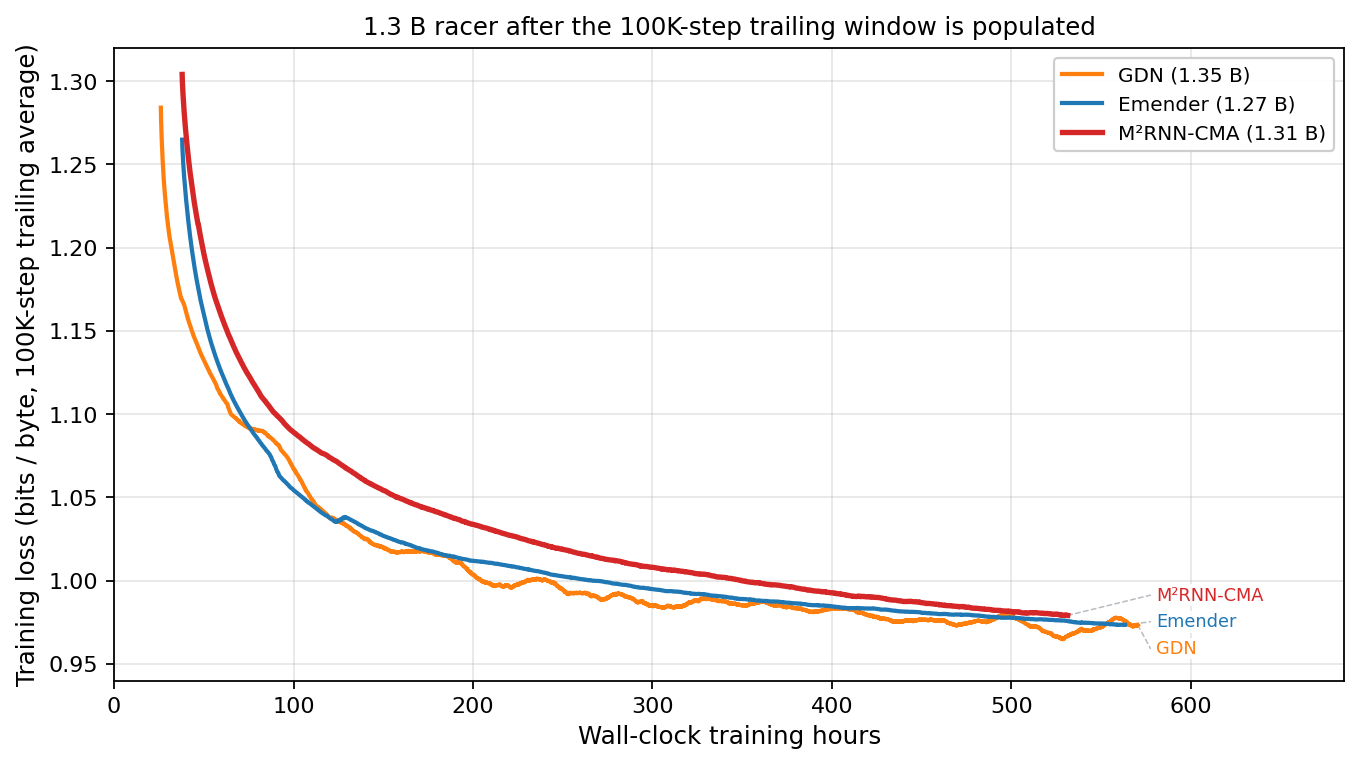
\includegraphics[width=0.95\linewidth]{assets/figure_2.png}
\caption{ \emph{Training-dynamics diagnostic for the 1.3 B comparison: training-loss-vs-wallclock trajectories on The Pile under matched per-architecture CMA-ES. These curves are a diagnostic of training dynamics, not the basis for the architecture comparison --- the reported measurement is the held-out bpb (below). All three trajectories occupy the same sub-1-bpb band; at their released v0.3 checkpoints E88 and GDN are at 0.973 BPB and M\textsuperscript{2}RNN-CMA at 0.979 across the sampled window.} Schedule-free AdamW on The Pile with a 2048-token context. The single panel uses linear wall-clock hours from the start of the run to each model's released v0.3 checkpoint step, but each curve is drawn only after the 100K-step trailing window is fully populated and the curve is inside the plotted BPB range. Curves are 100K-step trailing moving averages of training loss in bits per byte; the nats/token $\rightarrow $ bits/byte conversion uses the canonical $\text{bytes/token} =  3.92$ for \protect\path|p50k_base| on The Pile (Section~\ref{sec:appendix_bpb}). E88 is at 1.273 B parameters; M\textsuperscript{2}RNN-CMA at 1.307 B; GDN at 1.352 B; the three plotted models have trained about 22.1-23.8 GPU-days at their released v0.3 checkpoints. The plotted trajectory is one realization per architecture. These training-loss trajectories are a diagnostic; the architecture comparison rests on the held-out bpb (below) and the predecessor ablations and CMA-ES sweeps (250+ configs/architecture), not on these curves. The multi-week per-architecture training extent is the standard unit at this scale class. Endpoint values are 100K-step trailing averages read at each model's released v0.3 checkpoint step (E88 step 1,542,000; GDN step 2,031,000; M\textsuperscript{2}RNN-CMA step 1,491,000): E88 0.973 BPB, GDN 0.973 BPB, and M\textsuperscript{2}RNN-CMA 0.979 BPB. E88 and GDN remain in the same sub-1-bpb wallclock band. M\textsuperscript{2}RNN-CMA has higher loss than the other two across the sampled window. The paper-shape M\textsuperscript{2}RNN baseline (not shown) diverged at step 8,400. Color convention used throughout the paper: Emender = blue, GDN = orange, M\textsuperscript{2}RNN-CMA = red. Curves end at each model's released v0.3 checkpoint step --- the same checkpoints used for the held-out bpb below; training continued past these points. }\label{fig_lm_racers}
\end{figure}


After about 22--24 GPU-days, E88 reaches 0.973 bpb on The Pile, GDN 0.973, M\textsuperscript{2}RNN-CMA 0.979; all three are sub-1-bpb. These values are read at each model's released v0.3 checkpoint step (E88 1,542,000; GDN 2,031,000; M\textsuperscript{2}RNN-CMA 1,491,000), which are the canonical checkpoints reported throughout. The corresponding 100K-trailing training losses are 2.644 nats/token (E88, step 1,542,000), 2.644 (GDN, step 2,031,000), and 2.660 (M\textsuperscript{2}RNN-CMA, step 1,491,000). Under the training tokenizer (\protect\path|p50k_base| BPE) on The Pile, mean bytes per token is 3.92 over a 2000-sample sweep at the training context of 2048 tokens (Section~\ref{sec:appendix_bpb}), so $\text{bpb} =  \text{nats/token} \times  {\operatorname{log}}_{2}\frac{e }{\text{bytes/token}} \approx  \text{nats/token} \times  0.368$. These training-loss curves are a training-dynamics diagnostic, not the basis for the architecture comparison: the reported measurement is the held-out bpb (next subsection), where the three models are descriptively close, and the architectures separate on the Section~\ref{sec:expressivity} state-tracking probes rather than on bulk language-model bits-per-byte.


\subsection*{Held-out bits-per-byte: the three are descriptively close}


The loss-vs-wallclock curve above plots \emph{training-loss} bpb under the fixed canonical $\text{bytes/token} =  3.92$ normalization. To test whether that within-class ordering survives off the training stream, we separately measure \emph{held-out} bpb: each model's real negative log-likelihood, in nats, over a held-out Pile slice it never trained on, divided by the slice's real UTF-8 byte count --- tokenizer-invariant, with no 3.92 constant (method in Section~\ref{sec:appendix_bpb}). On the canonical 10 MB held-out slice (context 2048, stride 1024), Emender reaches \emph{0.966} held-out bpb, GDN \emph{0.966}, and M\textsuperscript{2}RNN-CMA \emph{0.961} --- all sub-1-bpb, and all at or slightly below their respective train-loss figures (0.973 / 0.973 / 0.979). These held-out numbers are measured at the same released v0.3 checkpoint steps as the train-loss figures above (E88 1,542,000; GDN 2,031,000; M\textsuperscript{2}RNN-CMA 1,491,000), so train-loss and held-out now sit on one canonical checkpoint per model; generalization is healthy with no held-out blow-up.

Held-out bpb and train-loss bpb are different objects --- different data \emph{and} different byte-normalization --- and are not directly comparable. Critically, the train-loss ordering does \emph{not} reproduce held-out. Across five independent held-out Pile slices drawn from random deep offsets across the 1.31 TB corpus, the three models sit inside a 0.006-bpb band of mean bpb, narrower than the largest cross-slice standard deviation (0.025 bpb); the between-model mean gaps are 0.05--0.31$\times $ the pooled cross-slice std. On held-out bulk bits-per-byte the three update rules are \emph{descriptively close}, not shown statistically equivalent by a seed-level or paired equivalence test. Which model is lowest is slice-dependent (lowest-bpb counts: Emender 0/5, GDN 1/5, M\textsuperscript{2}RNN-CMA 4/5), so bulk held-out perplexity shows descriptive closeness rather than tested equivalence at this budget. This is the expected reading: the architectures separate on the Section~\ref{sec:expressivity} state-tracking probes, not on bulk language-model bits-per-byte. Section~\ref{sec:appendix_bpb} places these numbers in the landscape of open Pile-trained models, out-of-distribution anchors, and classical compressors.


\subsection*{Narrow observed loss bands under matched compute}


The narrow observed bands occur under matched compute for each update rule. The three rules --- delta-correcting (E88), raw-write (M\textsuperscript{2}RNN-CMA), and linear (GDN) --- each received the \emph{same} per-architecture CMA-ES hyperparameter-and-shape search budget and were then trained to \emph{matched} FLOPs, and they converge to within $\approx  0.005$--$0.006$ bpb of one another on \emph{both} axes: held-out 0.966 / 0.966 / 0.961 and train-loss 0.973 / 0.973 / 0.979. Equal tuning effort and equal compute land three structurally different recurrences in the same narrow loss band.

After each family is tuned to its own best operating point, the converged losses occupy a narrow observed band; this does not establish equal loss across update rules. Where they come apart is the Section~\ref{sec:expressivity} state-tracking probes, not the reported bpb bands, and so far that separation shows only on synthetic algebraic state-tracking (${S }_{5}$/parity/FSM, Section~\ref{sec:expressivity}) --- tasks that \emph{no} model in the cohort solves. The non-synthetic signals --- bulk held-out loss, the QA panel, and the reasoning panel (Section~\ref{sec:lm}) --- occupy narrow observed bands, without a tested equivalence claim.

The loss figures of this appendix are single-seed per architecture. The five held-out Pile slices (Section~\ref{sec:appendix_bpb}) show slice-dependent ordering of the lowest-bpb model and narrow observed bands of between-model means; their cross-slice standard deviations do not measure uncertainty of a paired difference. The Common-Pile contamination control (Section~\ref{sec:appendix_bpb}) also shows descriptive closeness on a second distribution. These observations do not establish an architecture-agnostic compute-optimal loss at this matched FLOP budget. The state-tracking results that carry the paper do not rest on these single-seed loss runs: they rest on the 3-seed 8 M expressivity probes (Section~\ref{sec:expressivity}) and the 1.3 B length-generalization separation (below), where the architectures genuinely come apart.


\subsection*{1.3 B fine-tune study on the predecessor cohort}


The 8 M probes above have large state-count headroom; an inductive-bias interpretation is plausible but not guaranteed by those counts. The complementary question is whether the separation survives at the 1.3 B scale, in the trained checkpoints themselves. We fine-tune each released v0.3 checkpoint --- E88 (delta, 1.273 B), GDN (linear-recurrent, 1.352 B), and M\textsuperscript{2}RNN-CMA (raw-write, 1.307 B) --- on the ${S }_{3}$ and ${S }_{5}$ word problems and measure \emph{length generalization}: train on prefixes of length $T  \leq  64$, evaluate out to $T  =  512$ (8\ensuremath{\times} the longest trained length). The trainable harness is initialized by a strict weight-load of the public v0.3 checkpoint; a full held-out-slice load-sanity check reproduces each model's published readback to $\leq  1.3 \times  {10}^{- 4}$ nats, so the fine-tune is of the released artifact itself.

To keep the comparison about expressivity rather than trainability, each model is first driven \emph{to competence on the solvable tasks}: at the longest trained length $T  =  64$, E88 reaches parity 1.000 / ${S }_{3}$ 1.000, GDN 0.997 / 0.928, and M\textsuperscript{2}RNN 0.999 / 0.748 (${S }_{3}$ 0.990 at $T  =  32$). Under the identical matched recipe (lr $2 \times  {10}^{- 4}$, 2500 steps) the raw-write M\textsuperscript{2}RNN under-fits even solvable parity (0.557); reaching solvable competence took a gentler, longer recipe (lr $5 \times  {10}^{- 5}$, 12,000 steps) where E88 and GDN saturate the solvable tasks at lr $2 \times  {10}^{- 4}$ in $\leq  5000$ steps. This \emph{effort-to-competence} gap is the matched-FLOP efficiency statement at 1.3 B: raw-write needs more budget to reach the same solvable-task competence the delta update reaches cheaply.

That to-competence procedure removed the \emph{baseline's} trainability confound but left an asymmetry: M\textsuperscript{2}RNN got a gentler, longer recipe to reach competence while E88 never got the same extra budget on ${S }_{5}$, so E88's ${S }_{5}$ length-extrapolation shortfall (0.162 at $T  =  512$) was ambiguous between a real capacity ceiling and mere under-training. The headline run below \emph{fixes the asymmetry}: all three models get the \emph{same} a-priori recipe and the \emph{same}, larger, fixed budget on ${S }_{5}$: M\textsuperscript{2}RNN's exact gentle recipe (lr $5 \times  {10}^{- 5}$ constant) with the step count \emph{doubled} to 24,000 (2\ensuremath{\times} M\textsuperscript{2}RNN's to-competence budget), identical length curriculum $T  \leq  64$, and \emph{no} ${S }_{5}$-tuning (a single fixed step count, no early-stopping; constant LR so a flat curve cannot be confused with a decayed learning rate). The recipe was chosen and frozen before any ${S }_{5}$ result was seen. Table~\ref{tab_s5_1p3b} and Figure~\ref{fig_s5_symmetric} report where each model lands.


\begin{table}[htbp]
\centering
\begingroup\setlength{\tabcolsep}{3pt}
\begin{tabularx}{\linewidth}{|>{\hsize=1.71429\hsize\linewidth=\hsize\raggedright\arraybackslash}X|>{\hsize=0.85714\hsize\linewidth=\hsize\raggedright\arraybackslash}X|>{\hsize=0.85714\hsize\linewidth=\hsize\raggedright\arraybackslash}X|>{\hsize=0.85714\hsize\linewidth=\hsize\raggedright\arraybackslash}X|>{\hsize=0.85714\hsize\linewidth=\hsize\raggedright\arraybackslash}X|>{\hsize=0.85714\hsize\linewidth=\hsize\raggedright\arraybackslash}X|}\hline
\emph{Model} & \emph{${S }_{5}$ T=64} & \emph{${S }_{5}$ T=128} & \emph{${S }_{5}$ T=256} & \emph{${S }_{5}$ T=512} & \emph{${S }_{5}$ T=1024} \\ \hline
E88 (delta) & \emph{0.921} & \emph{0.536} & \emph{0.272} & \emph{0.143} & \emph{0.076} \\ \hline
M\textsuperscript{2}RNN (raw-write) & 0.658 & 0.335 & 0.172 & 0.090 & 0.049 \\ \hline
GDN (linear) & 0.117 & 0.063 & 0.035 & 0.022 & 0.015 \\ \hline
random & 0.0083 & 0.0083 & 0.0083 & 0.0083 & 0.0083 \\ \hline
\end{tabularx}
\endgroup

\caption{ \emph{${S }_{5}$ length-extrapolation at 1.3 B scale, symmetric 24,000-step budget; all three models, one identical a-priori recipe, no ${S }_{5}$-tuning.} Each released \protect\path|@v0.3| checkpoint is loaded strictly and full-fine-tuned on ${S }_{5}$ alone under a single fixed recipe (lr $5 \times  {10}^{- 5}$ constant, 24,000 steps $= $ 2\ensuremath{\times} M\textsuperscript{2}RNN's to-competence budget, identical length curriculum $T  \leq  64$, seed 42), chosen and frozen before any ${S }_{5}$ result was seen. $T  =  64$ is the longest trained length; columns to its right are extrapolation out to 16\ensuremath{\times} ($T  =  1024$). Chance is $\frac{1}{120} =  0.0083$. At the trained length E88 (delta) nearly solves the tested prefixes (0.921) while this GDN run under-fits them (0.117, far below competence); raw-write M\textsuperscript{2}RNN reaches 0.658. Under extrapolation all three degrade and E88 $> $ M\textsuperscript{2}RNN $> $ GDN at \emph{every} length, but E88 plateaus below ceiling (0.143 at $T  =  512$, flat from $\approx  12, 000$ steps) rather than tracking ${S }_{5}$ to arbitrary length. Source: \protect\path|paper/review/S5_SYMMETRIC_BUDGET.md|; data \protect\path|paper/review/s5_symmetric_data/{e88,m2rnn,gdn}.json|. }\label{tab_s5_1p3b}
\end{table}



\begin{figure}[htbp]
\centering
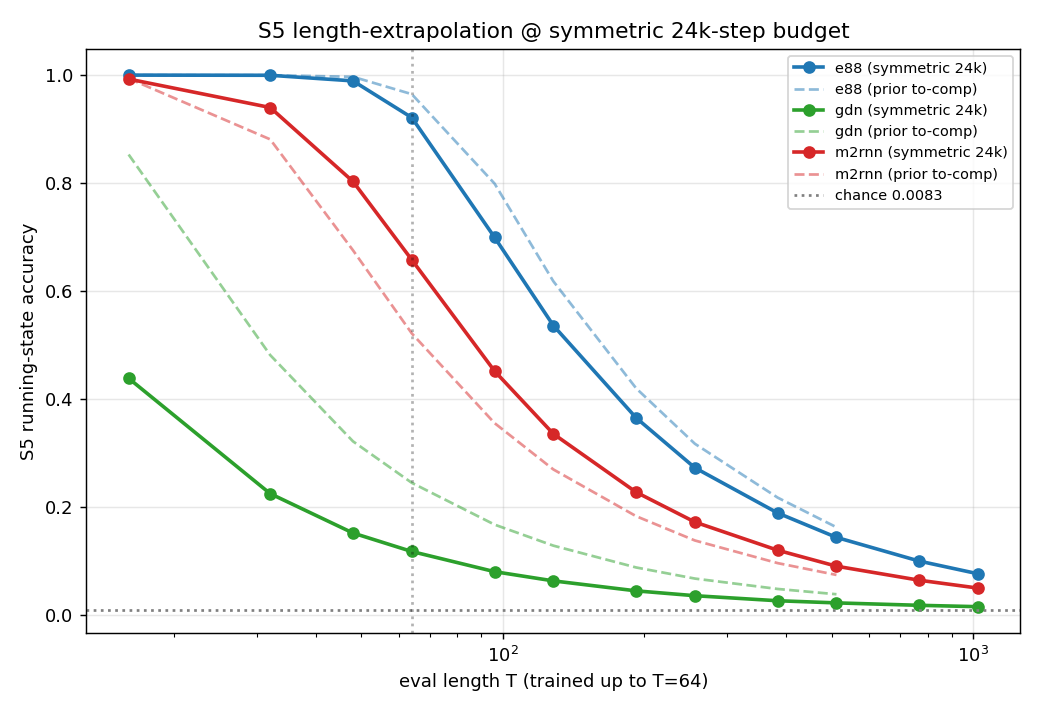
\includegraphics[width=0.95\linewidth]{assets/s5_symmetric_acc_vs_T.png}
\caption{ \emph{${S }_{5}$ length-extrapolation at the symmetric 24,000-step budget.} Running-state accuracy vs sequence length $T $ (log axis) for the three released 1.3 B architectures, each fine-tuned on ${S }_{5}$ under the \emph{same} a-priori recipe (lr $5 \times  {10}^{- 5}$ constant, 24,000 steps, no ${S }_{5}$-tuning): solid curves are this symmetric run (E88 blue, M\textsuperscript{2}RNN red, GDN green); faint dashed curves are the prior per-model to-competence run, shown for contrast. Trained on $T  \leq  64$ (vertical marker), evaluated out to $T  =  1024$ (16\ensuremath{\times} the longest trained length); chance is the dotted line ($\frac{1}{120}$). At the trained length the delta model nearly solves ${S }_{5}$ while this GDN run under-fits it; under extrapolation E88 $> $ M\textsuperscript{2}RNN $> $ GDN at \emph{every} length, with E88 plateauing below ceiling rather than tracking ${S }_{5}$ to arbitrary length. Numbers match Table~\ref{tab_s5_1p3b}. Real data: \protect\path|paper/review/s5_symmetric_data/{e88,m2rnn,gdn}.json|; figure generated by \protect\path|scripts/finetune_s5_symmetric.py| / \protect\path|scripts/analyze_s5_symmetric.py|. }\label{fig_s5_symmetric}
\end{figure}



\begin{figure}[htbp]
\centering
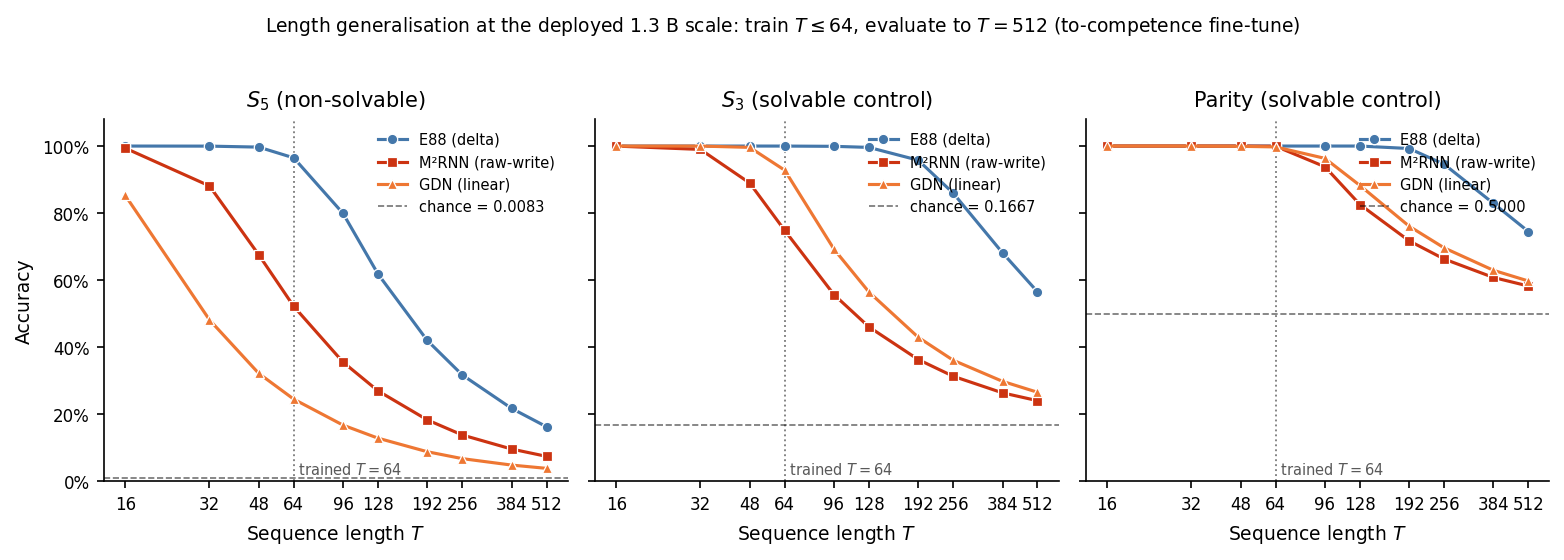
\includegraphics[width=0.95\linewidth]{assets/s5_s3_1p3b_lengthgen.png}
\caption{ \emph{Solvable controls and the prior to-competence ${S }_{5}$ cross-check at 1.3 B scale.} Accuracy vs sequence length $T $ for the three released architectures on the non-solvable ${S }_{5}$ probe (left) and the solvable ${S }_{3}$ and parity controls (center, right). All three are fine-tuned on $T  \leq  64$ (dotted marker) and evaluated out to $T  =  512$ --- 8\ensuremath{\times} the longest trained length; chance is the dashed line ($\frac{1}{120}$, $\frac{1}{6}$, $\frac{1}{2}$). Colors follow the paper convention (E88 blue, M\textsuperscript{2}RNN-CMA red, GDN orange). The ${S }_{5}$ panel here is the earlier per-model \emph{to-competence} run (the headline symmetric-budget ${S }_{5}$ result is Table~\ref{tab_s5_1p3b} / Figure~\ref{fig_s5_symmetric}); it is retained as a cross-check and reproduces the same E88 (delta) $> $ M\textsuperscript{2}RNN (raw-write) $> $ GDN (linear) ordering at \emph{every} length under a different recipe and budget: E88 degrades the most slowly (0.162 at $T  =  512$, far from solving), the linear GDN converges toward the chance floor, and raw-write tracks GDN's collapse shape. The ordering is consistent across both runs, but all three degrade with length and none tracks ${S }_{5}$ to arbitrary length. On the solvable controls all three are competent at the trained length and degrade only with extrapolation, motivating a structure-sensitive learning hypothesis without proving non-solvability causes the gap. Real data: \protect\path|paper/review/s3_s5_finetune_v03_data_tocomp/|; figure script: \protect\path|paper/figures/plot_s5_s3_1p3b_lengthgen.py|. }\label{fig_1p3b_lengthgen}
\end{figure}


\emph{Trained-length competence vs length-extrapolation plateau.} Two facts must be kept apart. First, \emph{at the trained length} ($T  =  64$) the delta model fits the held-out ${S }_{5}$ prefixes substantially better: E88 reaches 0.921, near-solving a non-solvable task, whereas this linear-recurrent GDN run under-fits it even at the trained length (0.117, far below competence) and raw-write M\textsuperscript{2}RNN reaches 0.658. Thus the delta update nearly solves the tested trained-length prefixes where this GDN run under-fits them; this is not an acquisition impossibility. Second, \emph{under length-extrapolation} (out to $T  =  1024$, 16\ensuremath{\times} the trained length) all three degrade; E88 degrades the slowest and stays strictly ahead at \emph{every} length, but it \emph{plateaus below ceiling} (0.143 at $T  =  512$, 0.076 at $T  =  1024$). This is a measured length-generalization plateau, not a proved capacity limit or expressive impossibility: the $T  =  512$ curve is flat from $\approx  12, 000$ steps at 2\ensuremath{\times} M\textsuperscript{2}RNN's budget under constant LR (see \emph{The delta update is also length-bounded} below). The accurate statement is therefore neither "E88 length-generalizes on ${S }_{5}$" nor "E88 fails ${S }_{5}$": the delta update learns ${S }_{5}$ at the trained length and leads at every length, with its length-extrapolation plateauing below ceiling at this width.

\emph{The historical GDN run plateaus.} GDN reaches 0.117 at trained length, 0.022 at $T = 512$, and 0.015 at $T = 1024$, near chance, with a flat curve by about step 6,000. The same run is stronger on parity and ${S }_{3}$. These are protocol-specific observations, not proof of a non-solvable computation barrier. The GDN2-MLP reversal in Section~\ref{sec:expressivity} and open constrained realizability question G3 prevent a families-wide interpretation.

\emph{Delta vs raw-write: a budget-robust ordering, not solve-vs-fail.} The symmetric run removes the recipe asymmetry directly. E88 received the \emph{same} doubled budget M\textsuperscript{2}RNN got, on the \emph{same} gentle recipe, with \emph{no} ${S }_{5}$-tuning, and still plateaus, so both confounds (M\textsuperscript{2}RNN's trainability deficit and E88's never-having-had-the-extra-budget) are bought out symmetrically. Under that symmetric budget raw-write M\textsuperscript{2}RNN fits the trained length less well than the delta model (0.658 vs 0.921) and stays below it at every extrapolation length (0.090 vs 0.143 at $T  =  512$; 0.049 vs 0.076 at $T  =  1024$), tracking the linear GDN's collapse shape far more than the delta model's. The ordering E88 $> $ M\textsuperscript{2}RNN $> $ GDN holds at \emph{every} length out to 16\ensuremath{\times} and is robust to a large budget swing: the matched 2,500-step (lr $2 \times  {10}^{- 4}$), the per-model to-competence, and this symmetric 24,000-step (lr $5 \times  {10}^{- 5}$) runs all land E88 $\approx  0.14$ at $T  =  512$ strictly ahead of M\textsuperscript{2}RNN $\approx  0.09$. The claim is therefore one of \emph{length-extrapolation efficiency}, not can/can't: at matched (indeed doubled) budget the delta update reaches strictly further with length than raw-write, and both \emph{nonlinear} updates plateau below ceiling as length grows.

\emph{The delta update also plateaus under these recipes.} E88's $T = 512$ accuracy is flat from about 12,000 steps under constant LR, and the three recipe variants converge near 0.14. This motivates studying length generalization; it does not isolate capacity from optimization. A late-rate extrapolation suggesting only about 0.03 further gain is not a measured doubled-budget result. The supported statement is that neither tested nonlinear arm reaches ceiling at extrapolated length, while E88 remains ahead under the recorded budgets.

\emph{Generalization beyond seen sequences.} Evaluation words are held out and test-disjoint; the generator alphabet gives exponentially many possible words. Above-chance accuracy out to $T = 1024$ supports learning transferable structure rather than memorizing the enumerated training examples. It does not establish exact algorithm recovery or exclude finite-context heuristics. The solvable controls are useful diagnostics, not a theorem that non-solvability causes the difference.

\emph{Raw-write's shortfall is partly trainability.} M\textsuperscript{2}RNN's ${S }_{5}$ (and ${S }_{3}$) accuracy was still slowly rising at 12,000 steps --- its curve is not the flat, converged ceiling GDN's is --- so its ${S }_{5}$ shortfall is partly entangled with optimization difficulty: full fine-tuning of the 1.3 B raw-write model is unstable and needed the gentler/longer recipe merely to fit parity. We therefore do \emph{not} claim a pure-expressivity wall for either raw-write or linear GDN; the statement here is the matched-FLOP efficiency one: raw-write needs more budget to approach what the delta update reaches cheaply, and within the budgets tested (including the symmetric doubled budget) it does not get there. The observations across the recorded recipes are (a) the clean expressivity contrast is delta E88 (fits the trained prefixes better, leads at every tested length) vs this GDN run (under-fits and plateaus under the tested recipes), and (b) raw-write M\textsuperscript{2}RNN, even at best-effort competence, exhibits the length-extrapolation collapse and stays below the delta update's reach at every length; as noted above, the delta update too plateaus below ceiling at this width.

\emph{The solvable controls hold (S3 and parity).} Figure~\ref{fig_1p3b_lengthgen} surfaces the two solvable controls alongside ${S }_{5}$. All three architectures are competent at the trained length on both: at $T  =  64$, parity is 1.000 / 0.997 / 0.999 and ${S }_{3}$ is 1.000 / 0.928 / 0.748 (E88 / GDN / M\textsuperscript{2}RNN), and they degrade only under extrapolation --- E88 still 0.565 on ${S }_{3}$ and 0.745 on parity at $T  =  512$. Competence on the solvable tasks makes a structure-sensitive learning explanation plausible, but does not isolate non-solvability from other differences in the task and recipe. (The raw-write M\textsuperscript{2}RNN's \emph{own} ${S }_{3}$ decay at length, falling below the linear GDN past $T  =  96$, is the same matched-FLOP efficiency story, not an expressivity wall --- its solvable-task curve was still rising; see \emph{Raw-write's shortfall is partly trainability} above.)


\subsection*{QA and reasoning panel at 1.3 B: parity-rate evidence}


For capability beyond loss numbers we evaluate the three 1.3 B-class models on a 300-item multi-choice continuation harness sampled from ARC-C/E \citep{arc2018}, HellaSwag \citep{hellaswag2019}, SciQ \citep{sciq2017}, OpenBookQA \citep{openbookqa2018}, and BoolQ \citep{boolq2019}. At the current training budget, E88 reaches 0.367 (random \ensuremath{~ }0.29), GDN 0.380, and M\textsuperscript{2}RNN-CMA 0.367; all three sit within one standard error of one another ($\text{SE} \approx  6$ pp at 50 items per task). On a separate reasoning panel (BIG-Bench Hard \citep{bbh2022}, ReCLor \citep{reclor2020}, FOLIO \citep{folio2022}), all three families collapse on multi-step object tracking (the seven-object shuffled-objects tracking task, 0.10--0.13, near-random) and on FOLIO/ReCLor (near-random for all three), with GDN leading on formal fallacies and web-of-lies. E88's overall reasoning accuracy (0.319) is within one standard error of M\textsuperscript{2}RNN-CMA (0.336). None has crossed the threshold where reasoning benchmarks differentiate, consistent with Section~\ref{sec:intro}'s class-level claim at this training budget. The state-tracking-specific reasoning separation, if it exists, will emerge at longer training horizons; Section~\ref{sec:predictions} states the prediction explicitly.


\section{Held-out bits-per-byte measurement (predecessor cohort)}\label{sec:appendix_bpb}


This appendix is the evidentiary backbone of the held-out descriptive closeness reported in Section~\ref{sec:appendix_cohort}: it documents exactly how the held-out bits-per-byte figures are measured and places them in a landscape of reference models and classical compressors. Every number is measured by the eval harness described below; none is re-fitted. The measurement code, slice manifests, and re-exported checkpoints are public (see the availability statement in Section~\ref{sec:conclusion}).


\subsection*{Tokenizer-invariant held-out bpb}


So that models with different tokenizers are comparable on identical bytes, held-out bpb is computed from each model's real summed negative log-likelihood over the slice and the slice's real UTF-8 byte count:


\[\begin{aligned}\text{bpb} =  ( {\text{total NLL}}_{\text{nats}} /  \operatorname{ln} 2)  /  \text{total UTF-8 bytes}. \end{aligned}\]


Each model uses its \emph{own} tokenizer, and the denominator is the shared byte count, so bytes/token is a \emph{measured} per-tokenizer quantity (4.00 for the GPT-NeoX BPE, 3.82 for our \protect\path|p50k_base| runs on the canonical slice) --- \emph{not} the fixed $\text{bytes/token} =  3.92$ constant used for the train-loss curve in Section~\ref{sec:lm}. The held-out and train-loss figures are therefore distinct objects: they differ in normalization as well as in the data scored. Every token is scored once under a sliding window (context 2048, stride 1024) with up to 2047 tokens of left context, the standard fixed-length-model perplexity recipe; out-of-distribution anchors GPT-2 XL and OPT-1.3B run at context 1024 (GPT-2 XL position limit). Pipeline: \protect\path|scripts/measure_pile_bpb.py| (open models) and \protect\path|scripts/measure_pile_bpb_elman.py| (our models, in-harness forward).

Algorithm 8 states the scoring order behind the held-out measurement. The denominator counts the shared source bytes once; overlapping context is not rescored. Correct schedule-free weight recovery and the first-block sanity check precede reporting, and a failure is not a numeric measurement.

\emph{Algorithm 8 --- tokenizer-invariant held-out evaluation.}
\begin{verbatim}
Input: sha-verified slice bytes, model, tokenizer, window/stride
1. Load the bound inference weights; apply required y-mode recovery.
2. Tokenize the slice with this model's tokenizer.
3. Run the first-block sanity gate; stop on failure.
4. Slide the context window; mask already scored target positions.
5. Sum next-token negative log-likelihood on newly scored positions.
6. Divide total NLL by log(2) and by the slice's UTF-8 byte count.
Return: bits per byte, token/byte counts, slice and weight identities
\end{verbatim}



\subsection*{Held-out slice provenance}


The canonical held-out slice is a whole-line 10 MB region (9,999,511 bytes, sha256 \protect\path|3e4241a9|\ldots{}\protect\path||) taken at byte offset ${10}^{12}$ (\ensuremath{\approx}76.5\% into the 1.31 TB Pile master file) --- a deep offset the 1.3 B runs' sub-one-epoch stream from the file start is least likely to have consumed. The five-slice robustness check of Section~\ref{sec:lm} adds four further independent, non-overlapping, sha-verified slices at offset fractions 0.137 / 0.341 / 0.523 / 0.911, each \ensuremath{\approx}10 MB and \ensuremath{\approx}2.5 M scored tokens. Identical bytes feed every model, so the byte denominator is shared and bpb is comparable across tokenizers. A block-loss sanity gate (mean nats/token on the first 2048-token block must lie in $[ 1.5,  4.0] $, model train loss \ensuremath{\approx}2.6) ran before any of our models' bpb was reported; all gated runs passed. The sha-verified slice manifests are released with the measurement code (see the Section~\ref{sec:conclusion} availability statement).


\subsection*{Second distribution: Common Pile (contamination control)}


Because the open Pile-trained references (Pythia, GPT-Neo) saw the Pile in training, their Pile numbers are effectively in-distribution. As an independent check we re-measure through the identical pipeline on a held-out slice of Common Pile (v0.1 main-mix; 9,999,606 bytes, document-aligned on the \protect\path|0x1E| record separator, at a random deep offset 65.5\% into its 1 TB corpus), a permissively-licensed corpus none of these models trained on. The Pile-trained models score within $\leq  0.003$ bpb of their Pile numbers there (Pythia-1.4B $+ 0.0028$, GPT-Neo-1.3B $+ 0.0002$, Pythia-1B $+ 0.0003$), so the Pile result is \emph{not} contamination-inflated. Our three models on the same Common-Pile slice measure Emender 0.981, GDN 0.963, M\textsuperscript{2}RNN-CMA 0.973 --- within \ensuremath{\approx}0.02 bpb of their Pile figures, with ordering GDN < M\textsuperscript{2}RNN-CMA < Emender (again not the train-loss ordering), consistent with a small distribution shift rather than a blow-up. Best classical coder on Common Pile is xz \ensuremath{- }9 at 2.061 bpb.


\subsection*{Checkpoints and reproducibility}


The three held-out checkpoints (Emender step 1,542,000; GDN 2,031,000; M\textsuperscript{2}RNN-CMA 1,491,000) are pinned to persistent storage with full schedule-free optimizer state and sha-verified. Recovering a correct inference forward from these schedule-free \citep{schedulefree2024} runs requires the \emph{y-mode} weight swap (load the optimizer state and call \protect\path|optimizer.train()|); the saved model weights alone are the eval-extrapolated \emph{x-mode} view and are catastrophic at inference (\ensuremath{\approx}18 nats/token). The public HuggingFace v0.3 release was re-exported with the corrected y-mode weights and verified, by a clean-cache readback from the hub through the bundled modeling code, to reproduce the held-out bpb to within $2 \times  {10}^{- 5}$ nats (Emender 0.96613, GDN 0.96612, M\textsuperscript{2}RNN-CMA 0.96132). Only the \protect\path|v0.3| revision carries this corrected re-export; the earlier public revisions (\protect\path|v0.1|, \protect\path|v0.2|) were shipped from the same schedule-free \emph{x-mode} pipeline, predate the fix, and are not usable for reproduction --- cite \protect\path|@v0.3| only.


\subsection*{Where the held-out bpb sits --- landscape, not a ranking}



\begin{table}[htbp]
\centering
\begingroup\setlength{\tabcolsep}{3pt}
\begin{tabularx}{\linewidth}{|>{\hsize=1.66667\hsize\linewidth=\hsize\raggedright\arraybackslash}X|>{\hsize=0.83333\hsize\linewidth=\hsize\raggedright\arraybackslash}X|>{\hsize=0.83333\hsize\linewidth=\hsize\raggedright\arraybackslash}X|>{\hsize=0.83333\hsize\linewidth=\hsize\raggedright\arraybackslash}X|>{\hsize=0.83333\hsize\linewidth=\hsize\raggedright\arraybackslash}X|}\hline
\emph{Tier} & \emph{Model / coder} & \emph{Params} & \emph{Held-out bpb} & \emph{Trained on Pile?} \\ \hline
Ours (matched budget) & Emender (E88) & 1.273 B & 0.966 & yes, \ensuremath{\approx}0.05 epoch \\ \hline
Ours (matched budget) & GDN & 1.352 B & 0.966 & yes, \ensuremath{\approx}0.05 epoch \\ \hline
Ours (matched budget) & M\textsuperscript{2}RNN-CMA & 1.307 B & 0.961 & yes, \ensuremath{\approx}0.05 epoch \\ \hline
Open Pile-trained & Pythia-1.4B & 1.42 B & 0.7157 & yes, \ensuremath{\approx}1 epoch (in-dist.) \\ \hline
Open Pile-trained & GPT-Neo-1.3B & 1.32 B & 0.7403 & yes, \ensuremath{\approx}1 epoch (in-dist.) \\ \hline
Open Pile-trained & Pythia-1B & 1.01 B & 0.7423 & yes, \ensuremath{\approx}1 epoch (in-dist.) \\ \hline
Familiar OOD & OPT-1.3B & 1.32 B & 0.8615 & no (OOD) \\ \hline
Familiar OOD & GPT-2 XL & 1.56 B & 1.0137 & no (OOD) \\ \hline
Classical & xz \ensuremath{- }9 (LZMA) & --- & 2.190 & n/a (model-free) \\ \hline
Classical & gzip \ensuremath{- }9 (DEFLATE) & --- & 2.803 & n/a (model-free) \\ \hline
\end{tabularx}
\endgroup

\caption{ \emph{Held-out bits-per-byte landscape --- context, not an architecture ranking.} All neural numbers are tokenizer-invariant held-out bpb on the canonical 10 MB Pile slice; classical coders are single-stream over the same bytes. The vertical ordering is \emph{dominated by training budget and train/test distribution, not by the update rule}, and must not be read as a quality verdict. Our three models trained on \ensuremath{\approx}15--16 B tokens (\ensuremath{\approx}0.05 epoch of the Pile); the open Pile-trained references saw \ensuremath{\approx}10--20$\times $ more (\ensuremath{\approx}1 epoch, \ensuremath{\approx}300 B tokens) \emph{and} are in-distribution on this slice (it is effectively training data for them --- possible contamination), so their 0.72--0.74 is closer to a train-loss than a held-out number. The OOD anchors (OPT, GPT-2 XL) are out-of-distribution on the Pile, so their higher bpb is expected and is not a quality knock; GPT-2 XL measures 1.0137 here versus the Pile paper's published 1.0468 \citep{thepile2020}, a \ensuremath{\approx}0.03-bpb pipeline check confirming this single slice reads slightly low against the full Pile test set. The architecture-focused comparison is the matched-budget three-way at the top, which Section~\ref{sec:appendix_cohort} reports as descriptively close, not as a statistical equivalence result. }\label{tab_bpb_landscape}
\end{table}



\bibliographystyle{tmlr}
\bibliography{refs}

\end{document}
